\documentclass{vkr}
\usepackage[english, russian]{babel} % переносы
\usepackage{graphicx} % для вставки картинок
\graphicspath{{images/}} % путь к изображениям
\usepackage[hidelinks]{hyperref}
\usepackage{enumitem}
\usepackage{pdflscape}
\usepackage{float} % определяет метод H для рисунка с переносом на следующую страницу, ели не помещается
\usepackage{pdflscape}
\addto{\captionsrussian}{\renewcommand{\refname}{СПИСОК ИСПОЛЬЗОВАННЫХ ИСТОЧНИКОВ}}
\usepackage{xltabular} % для вставки таблиц
\usepackage{makecell}
\renewcommand\theadfont{} % шрифт в /thead
\usepackage{array} % для определения новых типов столбцов таблиц
\newcolumntype{T}{>{\centering\arraybackslash}X} % новый тип столбца T - автоматическая ширина столбца с выравниванием по центру
\newcolumntype{R}{>{\raggedleft\arraybackslash}X} % новый тип столбца R - автоматическая ширина столбца с выравниванием по правому краю
\newcolumntype{C}[1]{>{\centering\let\newline\\\arraybackslash\hspace{0pt}}m{#1}} % новый тип столбца C - фиксированная ширина столбца с выравниванием по центру
\newcolumntype{r}[1]{>{\raggedleft\arraybackslash}p{#1}} % новый тип столбца r - фиксированная ширина столбца с выравниванием по правому краю
\newcommand{\centrow}{\centering\arraybackslash} % командой \centrow можно центрировать одну ячейку (заголовок) в столбце типа X или p, оставив в оcтальных ячейках другой тип выравнивания
\newcommand{\finishhead}{\endhead\hline\endlastfoot}
\newcommand{\continuecaption}[1]{\captionsetup{labelformat=empty} \caption[]{#1}\\ \hline }
\usepackage{etoolbox}
\AtBeginEnvironment{xltabular}{\refstepcounter{tablecnt}} % подсчет таблиц xltabular, обычные таблицы подсчитываются в классе

\usepackage[tableposition=top]{caption} % подпись таблицы вверху
\captionsetup{strut=off}
\setlength{\intextsep}{0pt} % Vertical space above & below [h] floats
\setlength{\textfloatsep}{0pt} % Vertical space below (above) [t] ([b]) floats
\DeclareCaptionLabelFormat{gostfigure}{Рисунок #2} %подпись рисунка
\DeclareCaptionLabelFormat{gosttable}{Таблица #2} %подпись таблицы
\DeclareCaptionLabelSeparator{gost}{~--~} %разделитель в рисунках и таблицах
\captionsetup{labelsep=gost}
\captionsetup[figure]{aboveskip=10pt,belowskip=4mm,justification=centering,labelformat=gostfigure} % настройка подписи рисунка
\captionsetup[table]{font={stretch=1.41},skip=0pt,belowskip=0pt,aboveskip=8.5pt,singlelinecheck=off,labelformat=gosttable} % настройка подписи таблицы

\setlength{\LTpre}{8mm} % отступ сверху таблицы
\setlength{\LTpost}{6mm} % отступ снизу таблицы

\usepackage{enumitem}
\setlist{nolistsep,wide=\parindent,itemindent=*} % отступы вокруг списков, выравнивание с учетом разделителя

\usepackage{color} %% это для отображения цвета в коде
\usepackage{listings} %% листинги кода
\setmonofont[Scale=0.7]{Verdana} % моноширный шрифт для листинга

\definecolor{codegreen}{rgb}{0,0.6,0}
\definecolor{codegray}{rgb}{0.5,0.5,0.5}
\definecolor{codepurple}{rgb}{0.58,0,0.82}

\lstset{ %
language=C,                 % выбор языка для подсветки (здесь это С)
numbers=left,               % где поставить нумерацию строк (слева\справа)
numberstyle=\tiny,           % размер шрифта для номеров строк
stepnumber=1,                   % размер шага между двумя номерами строк
numbersep=5pt,                % как далеко отстоят номера строк от подсвечиваемого кода
commentstyle=\color{codegreen},
keywordstyle=\color{magenta},
numberstyle=\tiny\color{codegray},
stringstyle=\color{codepurple},
basicstyle=\linespread{0.95}\ttfamily,
backgroundcolor=\color{white}, % цвет фона подсветки - используем \usepackage{color}
showspaces=false,            % показывать или нет пробелы специальными отступами
showstringspaces=false,      % показывать или нет пробелы в строках
showtabs=false,             % показывать или нет табуляцию в строках
frame=single,              % рисовать рамку вокруг кода
tabsize=2,                 % размер табуляции по умолчанию равен 2 пробелам
captionpos=t,              % позиция заголовка вверху [t] или внизу [b] 
breaklines=true,           % автоматически переносить строки (да\нет)
breakatwhitespace=false, % переносить строки только если есть пробел
escapeinside={\%*}{*)}   % если нужно добавить комментарии в коде
}

\makeatletter % чтобы допускались русские комментарии в листингах
\lst@InputCatcodes
\def\lst@DefEC{%
 \lst@CCECUse \lst@ProcessLetter
  ^^80^^81^^82^^83^^84^^85^^86^^87^^88^^89^^8a^^8b^^8c^^8d^^8e^^8f%
  ^^90^^91^^92^^93^^94^^95^^96^^97^^98^^99^^9a^^9b^^9c^^9d^^9e^^9f%
  ^^a0^^a1^^a2^^a3^^a4^^a5^^a6^^a7^^a8^^a9^^aa^^ab^^ac^^ad^^ae^^af%
  ^^b0^^b1^^b2^^b3^^b4^^b5^^b6^^b7^^b8^^b9^^ba^^bb^^bc^^bd^^be^^bf%
  ^^c0^^c1^^c2^^c3^^c4^^c5^^c6^^c7^^c8^^c9^^ca^^cb^^cc^^cd^^ce^^cf%
  ^^d0^^d1^^d2^^d3^^d4^^d5^^d6^^d7^^d8^^d9^^da^^db^^dc^^dd^^de^^df%
  ^^e0^^e1^^e2^^e3^^e4^^e5^^e6^^e7^^e8^^e9^^ea^^eb^^ec^^ed^^ee^^ef%
  ^^f0^^f1^^f2^^f3^^f4^^f5^^f6^^f7^^f8^^f9^^fa^^fb^^fc^^fd^^fe^^ff%
  ^^^^20ac^^^^0153^^^^0152%
  % Basic Cyrillic alphabet coverage
  ^^^^0410^^^^0411^^^^0412^^^^0413^^^^0414^^^^0415^^^^0416^^^^0417%
  ^^^^0418^^^^0419^^^^041a^^^^041b^^^^041c^^^^041d^^^^041e^^^^041f%
  ^^^^0420^^^^0421^^^^0422^^^^0423^^^^0424^^^^0425^^^^0426^^^^0427%
  ^^^^0428^^^^0429^^^^042a^^^^042b^^^^042c^^^^042d^^^^042e^^^^042f%
  ^^^^0430^^^^0431^^^^0432^^^^0433^^^^0434^^^^0435^^^^0436^^^^0437%
  ^^^^0438^^^^0439^^^^043a^^^^043b^^^^043c^^^^043d^^^^043e^^^^043f%
  ^^^^0440^^^^0441^^^^0442^^^^0443^^^^0444^^^^0445^^^^0446^^^^0447%
  ^^^^0448^^^^0449^^^^044a^^^^044b^^^^044c^^^^044d^^^^044e^^^^044f%
  ^^^^0401^^^^0451%
  %%%
  ^^00}
\lst@RestoreCatcodes
\makeatother

\ВКРtrue
%\Практикаtrue
%\Курсоваяtrue

\newcommand{\Дисциплина}{<<Проектирование и архитектура программных систем>>} % для курсовой
\newcommand{\КодСпециальности}{09.03.04} % Курсовая
\newcommand{\Специальность}{Программная инженерия} % Курсовая
\newcommand{\Тема}{Веб-приложение для компьютерной поддержки самостоятельной работы} % ВКР Курсовая
\newcommand{\ТемаВтораяСтрока}{иностранных студентов при изучении языка программирования  JavaScript}
\newcommand{\ГдеПроводитсяПрактика}{ООО <<Предприятие ВТИ-Сервис>>} % для практики
\newcommand{\РуководительПрактПредпр}{Федосов Д. В.} % для практики
\newcommand{\ДолжнРуководительПрактПредпр}{директор} % для практики
\newcommand{\РуководительПрактУнивер}{Чаплыгин А. А.} % для практики
\newcommand{\ДолжнРуководительПрактУнивер}{к.т.н. доцент} % для практики
\newcommand{\Автор}{И. А. Седых}
\newcommand{\АвторРод}{Седых И.А.}
\newcommand{\АвторПолностьюРод}{Седых Ивана Александровича} % для практики
\newcommand{\Шифр}{21-06-0028}
\newcommand{\Курс}{4 } % для практики
\newcommand{\Группа}{ПО-11б}
\newcommand{\Руководитель}{Е. И. Аникина} % для ВКР и курсовой
\newcommand{\Нормоконтроль}{А. А. Чаплыгин} % для ВКР
\newcommand{\ЗавКаф}{А. В. Малышев} % для ВКР
\newcommand{\ДатаПриказа}{«04» апреля 2025~г.} % для ВКР
\newcommand{\НомерПриказа}{1696-с} % для ВКР
\newcommand{\СрокПредоставления}{«09» июня 2025~г.} % для ВКР, курсового

\begin{document}
\maketitle
\ifПрактика{}\else{
   \newpage
\begin{center}
\large\textbf{Минобрнауки России}

\large\textbf{Юго-Западный государственный университет}
\vskip 1em
\normalsize{Кафедра программной инженерии}
\vskip 1em
\ifВКР{
        \begin{flushright}
        \begin{tabular}{p{.4\textwidth}}
        \centrow УТВЕРЖДАЮ: \\
        \centrow Заведующий кафедрой \\
        \hrulefill \\
        \setarstrut{\footnotesize}
        \centrow\footnotesize{(подпись, инициалы, фамилия)}\\
        \restorearstrut
        «\underline{\hspace{1cm}}»\label{{\tiny }}
        \underline{\hspace{3cm}}
        20\underline{\hspace{1cm}} г.\\
        \end{tabular}
        \end{flushright}
        }\fi
\end{center}
\vspace{1em}
  \begin{center}
  \large
\ifВКР{
ЗАДАНИЕ НА ВЫПУСКНУЮ КВАЛИФИКАЦИОННУЮ РАБОТУ
  ПО ПРОГРАММЕ БАКАЛАВРИАТА}
  \else
ЗАДАНИЕ НА КУРСОВУЮ РАБОТУ (ПРОЕКТ)
\fi
\normalsize
  \end{center}
\vspace{1em}
{\parindent0pt
  Студента \АвторРод, шифр\ \Шифр, группа \Группа
  
1. Тема «\Тема\ \ТемаВтораяСтрока»
\ifВКР{
утверждена приказом ректора ЮЗГУ от \ДатаПриказа\ № \НомерПриказа
}\fi.

2. Срок предоставления работы к защите \СрокПредоставления

3. Исходные данные для создания программной системы:

3.1. Перечень решаемых задач:}

\renewcommand\labelenumi{\theenumi)}

\begin{enumerate}
\item Проанализировать требования к обучающим платформам и определить функциональные возможности для ролей преподавателей и студентов;
\item Разработать концептуальную модель веб-приложения для управления образовательным процессом, включая создание курсов, уроков, тестов и отслеживание прогресса;
\item Спроектировать программную систему на основе фреймворка Django с использованием реляционной базы данных и интерактивных веб-технологий;
\item Реализовать и протестировать программную систему, обеспечив корректную работу функционала для всех типов пользователей.
\end{enumerate}

{\parindent0pt
  3.2. Входные данные и требуемые результаты для программы:}

\begin{enumerate}

	\item Данные пользователей: информация о студентах и преподавателях (имя, email, роль, пароль).
	\item Данные курсов: название, описание, изображение, статус активности.
	\item Данные уроков: заголовок, описание, контент, ссылки на видео, упражнения, порядок отображения.
	\item Данные тестов: название, описание, минимальный проходной балл, вопросы (текст, тип: одиночный выбор, множественный выбор, текстовый ответ), варианты ответов и их корректность.
	\item Данные достижений: название, описание, условия присвоения.
	\item Данные прогресса: записи студентов на курсы, статус завершения уроков, результаты тестов.

\end{enumerate}

{\parindent0pt

  4. Содержание работы (по разделам):
  
  4.1. Введение.
  
  4.1. Анализ предметной области.
  
4.2. Техническое задание: основание для разработки, назначение разработки,
требования к программной системе, требования к оформлению документации.

4.3. Технический проект: общие сведения о программной системе, проект
данных программной системы, проектирование архитектуры программной системы, проектирование пользовательского интерфейса программной системы.

4.4. Рабочий проект: спецификация компонентов и классов программной системы, тестирование программной системы, сборка компонентов программной системы.

4.5. Заключение.

4.6. Список использованных источников.

5. Перечень графического материала:

\списокПлакатов

\vskip 2em
\begin{tabular}{p{6.8cm}C{3.8cm}C{4.8cm}}
Руководитель \ifВКР{ВКР}\else работы (проекта) \fi & \lhrulefill{\fill} & \fillcenter\Руководитель\\
\setarstrut{\footnotesize}
& \footnotesize{(подпись, дата)} & \footnotesize{(инициалы, фамилия)}\\
\restorearstrut
Задание принял к исполнению & \lhrulefill{\fill} & \fillcenter\Автор\\
\setarstrut{\footnotesize}
& \footnotesize{(подпись, дата)} & \footnotesize{(инициалы, фамилия)}\\
\restorearstrut
\end{tabular}
}

\renewcommand\labelenumi{\theenumi.}

   \abstract{РЕФЕРАТ}

Объем работы равен \formbytotal{lastpage}{страниц}{е}{ам}{ам}. Работа содержит \formbytotal{figurecnt}{иллюстраци}{ю}{и}{й}, \formbytotal{tablecnt}{таблиц}{у}{ы}{}, \arabic{bibcount} библиографических источников и \formbytotal{числоПлакатов}{лист}{}{а}{ов} графического материала. Количество приложений – 2. Графический материал представлен в приложении А. Фрагменты исходного кода представлены в приложении Б.

Перечень ключевых слов: обучающая платформа, веб-приложение, Django, мультиязычность, CKEditor, AOS, JavaScript, курсы, уроки, тесты, достижения, база данных, ORM, иностранные студенты, веб-интерфейс.

Объектом разработки является веб-приложение -- обучающая платформа, предназначенная для компьютерной поддержки самостоятельной работы иностранных студентов при изучении языка программирования JavaScript, с мультиязычным интерфейсом и интерактивными инструментами для обучения.

Целью выпускной квалификационной работы является создание удобной и функциональной платформы для самостоятельного изучения языка программирования JavaScript иностранными студентами, обеспечивающей доступ к образовательным материалам, тестированию и отслеживанию прогресса, способствующий повышению вовлечённости и эффективности обучения.

В процессе создания платформы были выделены основные сущности, использованы классы и методы Django, разработаны разделы для управления курсами, аналитикой прогресса и достижений, реализованы интерактивные элементы с использованием CKEditor для редактирования учебного контента.

При разработке платформы использовался фреймворк Django с интегрированными библиотеками для аутентификации, шаблонизации, обработки форм и мультиязычности, а также CKEditor и AOS для обеспечения интерактивности и удобства работы с учебным контентом.

Разработанная платформа была успешно протестирована и внедрена в систему обучения.

\selectlanguage{english}
\abstract{ABSTRACT}
  
The volume of work is \formbytotal{lastpage}{page}{}{s}{s}. The work contains \formbytotal{figurecnt}{illustration}{}{s}{s}, \formbytotal{tablecnt}{table}{}{s}{s}, \arabic{bibcount} bibliographic sources and \formbytotal{числоПлакатов}{sheet}{}{s}{s} of graphic material. The number of applications is 2. The graphic material is presented in annex A. The layout of the site, including the connection of components, is presented in annex B.

List of keywords: learning platform, web application, Django, multilingualism, CKEditor, AOS, JavaScript, courses, lessons, tests, achievements, administrator, user, web interface.

The object of development is a web application -- a learning platform designed for computer support of international students' independent work when learning the JavaScript programming language, with a multi-lingual interface and interactive learning tools.

The aim of the final qualification work is to create a convenient and functional platform for independent learning of JavaScript programming language by foreign students, providing access to educational materials, testing and progress tracking through a multi-lingual interface, which contributes to increased involvement and efficiency of learning.

In the process of creating the platform, the main entities were identified by designing data models, Django classes and methods were used to ensure work with entities related to JavaScript learning and correct functioning of the web application, sections for managing courses, lessons, JavaScript tests, progress and achievements analytics were developed, interactive elements were implemented using CKEditor for editing learning content and AOS for interface animation.

The Django framework with integrated libraries for authentication, templating, form processing and multi-language, as well as CKEditor and AOS for interactivity and usability of the learning content were used in the development of the platform.

The developed platform was successfully tested and implemented in the training system.
\selectlanguage{russian}
}\fi
\tableofcontents
\section*{ОБОЗНАЧЕНИЯ И СОКРАЩЕНИЯ}

БД -- база данных.

ИС -- информационная система.

ИТ -- информационные технологии. 

КТС -- комплекс технических средств.

ОМТС -- отдел материально-технического снабжения. 

ПО -- программное обеспечение.

РП -- рабочий проект.

СУБД -- система управления базами данных.

ТЗ -- техническое задание.

ТП -- технический проект.

UML (Unified Modelling Language) -- язык графического описания для объектного моделирования в области разработки программного обеспечения.

HTML (HyperText Markup Language) -- язык гипертекстовой разметки.

JavaScript -- язык программирования для веб-разработки.

CSS (Cascading Style Sheets) -- каскадные таблицы стилей.

SCSS (Sassy CSS) -- препроцессор, расширяющий возможности CSS.

UI (User Interface) -- пользовательский интерфейс.

UX (User Experience) -- пользовательский опыт.

REST API (Representational State Transfer Application Programming Interface) -- интерфейс программирования приложений, использующий архитектурный стиль REST.

CRUD (Create, Read, Update, Delete) -- основные операции для работы с данными.

MVC (Model-View-Controller) -- архитектурный шаблон проектирования.

PostgreSQL -- объектно-реляционная система управления базами данных с открытым исходным кодом.

JSON (JavaScript Object Notation) -- текстовый формат обмена данными.
\ifПрактика{}\else{\section*{ВВЕДЕНИЕ}
\addcontentsline{toc}{section}{ВВЕДЕНИЕ}

Современные информационные технологии играют ключевую роль в образовательном процессе, обеспечивая доступ к учебным материалам и поддерживая самостоятельное обучение. Обучающие платформы становятся важным инструментом для изучения программирования, особенно для иностранных студентов, которым требуется гибкий и доступный формат обучения с учетом языковых особенностей. Язык программирования JavaScript является одним из наиболее востребованных в веб-разработке благодаря своей универсальности и широкому применению в создании интерактивных веб-приложений. Разработка специализированных веб-приложений для обучения JavaScript позволяет эффективно организовать процесс самостоятельной работы студентов, предоставляя структурированные курсы, интерактивные тесты и отслеживание прогресса.

Веб-приложение, ориентированное на иностранных студентов, предполагает использование мультиязычного интерфейса и интерактивных инструментов, таких как редакторы контента и анимации, для повышения вовлеченности и удобства обучения. Такие платформы позволяют студентам изучать JavaScript в удобном темпе, а преподавателям — эффективно управлять образовательным контентом и отслеживать результаты.

Создание веб-приложения для обучения программированию способствует не только повышению квалификации студентов, но и расширению доступности образования для международной аудитории. Платформа становится инструментом, который объединяет образовательные ресурсы, тестирование и аналитику в единой цифровой среде, упрощая процесс обучения и делая его более интерактивным.

\emph{Цель настоящей работы} – разработка веб-приложения для компьютерной поддержки самостоятельной работы иностранных студентов при изучении языка программирования JavaScript, обеспечивающего доступ к образовательным материалам, тестированию и отслеживанию прогресса через мультиязычный интерфейс для повышения эффективности обучения. Для достижения поставленной цели необходимо решить следующие задачи:
\begin{itemize}
	\item провести анализ предметной области и требований к обучающим платформам для иностранных студентов;
	\item разработать концептуальную модель веб-приложения для обучения JavaScript;
	\item спроектировать веб-приложение с учетом мультиязычности и интерактивности;
	\item реализовать веб-приложение средствами современных веб-технологий.
\end{itemize}

\emph{Структура и объем работы.} Отчет состоит из введения, 4 разделов основной части, заключения, списка использованных источников, 2 приложений. Текст выпускной квалификационной работы равен \formbytotal{lastpage}{страниц}{е}{ам}{ам}.

\emph{Во введении} сформулирована цель работы, поставлены задачи разработки, описана структура работы, приведено краткое содержание каждого из разделов.

\emph{В первом разделе} на стадии анализа предметной области приводится сбор информации о требованиях к обучающим платформam's для иностранных студентов, изучающих JavaScript, и особенностях организации самостоятельной работы.

\emph{Во втором разделе} на стадии технического задания приводятся требования к разрабатываемому веб-приложению, включая поддержку мультиязычности и интерактивных элементов.

\emph{В третьем разделе} на стадии технического проектирования представлены проектные решения для веб-приложения, включая модели данных и структуру интерфейса.

\emph{В четвертом разделе} приводится список классов и их методов, использованных при разработке платформы, а также результаты тестирования разработанного веб-приложения.

В заключении излагаются основные результаты работы, полученные в ходе разработки.

В приложении А представлен графический материал.
В приложении Б представлены фрагменты исходного кода. 
}\fi
\section{Анализ предметной области}
\subsection{Принцип работы программно-информационной системы управления обучением}

В условиях глобализации образовательных процессов и роста числа иностранных студентов, изучающих программирование, возникает потребность в специализированных программных системах, обеспечивающих поддержку самостоятельного обучения. Согласно международным стандартам качества образования, такие системы должны предоставлять доступ к учебным материалам, автоматизировать проверку знаний и учитывать языковые особенности пользователей. Веб-приложение для компьютерной поддержки самостоятельной работы иностранных студентов при изучении языка программирования JavaScript позволяет автоматизировать ключевые процессы обучения. Рассмотрим основные из них:

\subsubsection{Управление курсами}
После создания курса преподавателем через интерфейс системы, он становится доступным для записи студентов. Курс включает уроки и тесты, которые автоматически отображаются в панели студента. Студент может записаться на курс, просмотреть его содержание и начать обучение. Система фиксирует прогресс студента, а данные о записи передаются в базу данных SQLite для дальнейшей аналитики.

\subsubsection{Управление уроками}
Преподаватели могут добавлять уроки через форму, редактировать их и сортировать с помощью Sortable.js. Каждый урок содержит описание, материалы и тесты. Система автоматически проверяет доступность урока для студента: доступ к следующему уроку открывается только после выполнения теста предыдущего урока. Уроки поддерживают локализацию через Django i18n, что позволяет иностранным студентам выбирать язык интерфейса.


\subsubsection{Управление тестами}
Система автоматизирует создание и управление тестами. Преподаватель может добавлять вопросы и ответы, указывать правильные варианты и проходной балл. Студенты проходят тесты через интерфейс урока, а система автоматически подсчитывает баллы и фиксирует результаты. Для иностранных студентов предусмотрена локализация вопросов и ответов, что упрощает процесс тестирования.

\subsubsection{Аналитика и результаты}
Для анализа успеваемости студентов система предоставляет модуль управления результатами. Преподаватель может просматривать результаты тестов, включая средний балл, максимальный и минимальный, а также удалять их при необходимости. Студенты получают доступ к своим результатам через панель, что позволяет отслеживать прогресс. Данные хранятся в базе SQLite и доступны для аналитики. 

\subsubsection{Поддержка пользователей} 
Система включает модуль управления пользователями, который поддерживает регистрацию студентов и преподавателей. Для иностранных студентов предусмотрена смена языка интерфейса через Django i18n, что обеспечивает комфортное использование. Также система фиксирует роли пользователей и ограничивает доступ к функционалу через декораторы.


\subsection{Компоненты программно-информационной системы управления обучением}
Программно-информационная система управления обучением представляет собой комплекс взаимодействующих программных модулей, аппаратных средств и технологий, предназначенных для хранения, обработки и предоставления образовательного контента. Важным условием функционирования системы является наличие интернет-соединения, обеспечивающего взаимодействие между клиентской и серверной частями. Для обеспечения безопасности данных используется аутентификация через Django contrib.auth, а также защита маршрутов (@loginrequired). На рисунке ~\ref{system:image} представлена схема взаимодействия компонентов системы управления обучением, а также способы их взаимодействия. 

\begin{figure}[ht]
	\centering
	\center{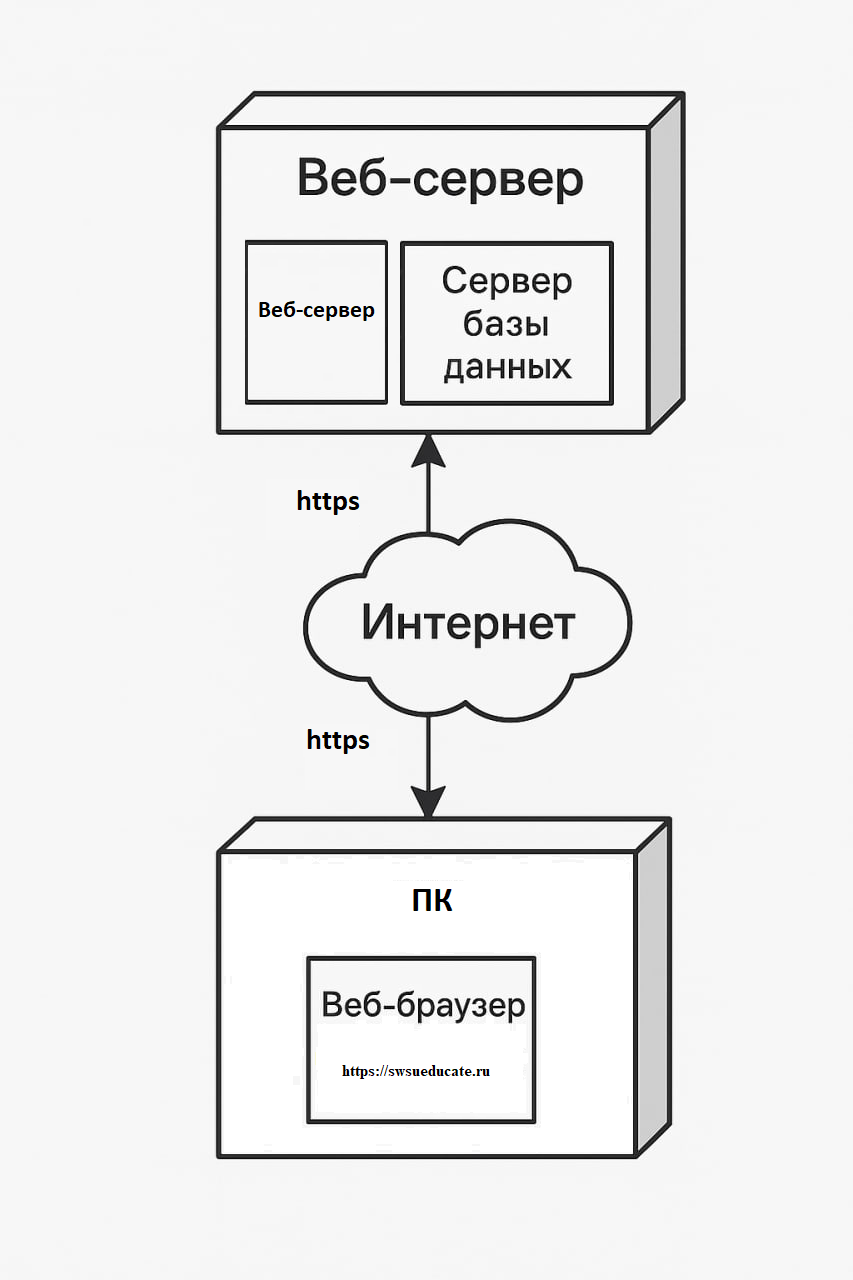
\includegraphics[width=0.6\linewidth]{images/диаграмма2}} 
	\caption{Схема взаимодействия компонентов системы управления обучением}
	\label{system:image}
\end{figure}


\subsection{Отчёты успеваемости}
Одной из причин использования веб-приложения в образовательных целях является удобство формирования отчётов об успеваемости. В системе предусмотрен модуль аналитики, в котором представлена статистическая информация для таких категорий, как прогресс студентов, результаты тестов и активность пользователей. Рассмотрим ключевой отчёт:

\subsubsection{Отчёт по результатам тестов}
Отчёт по результатам тестов представляет собой документ, фиксирующий итоги выполнения тестов студентами за определённый период. Он формирует данные о баллах на момент начала и завершения теста, сведения об общем количестве попыток (attemptnumber), информацию о проходном балле, а также статистику: средний, максимальный и минимальный балл. Пример отчёта представлен на рисунке. 

\begin{figure}[ht]
	\centering
	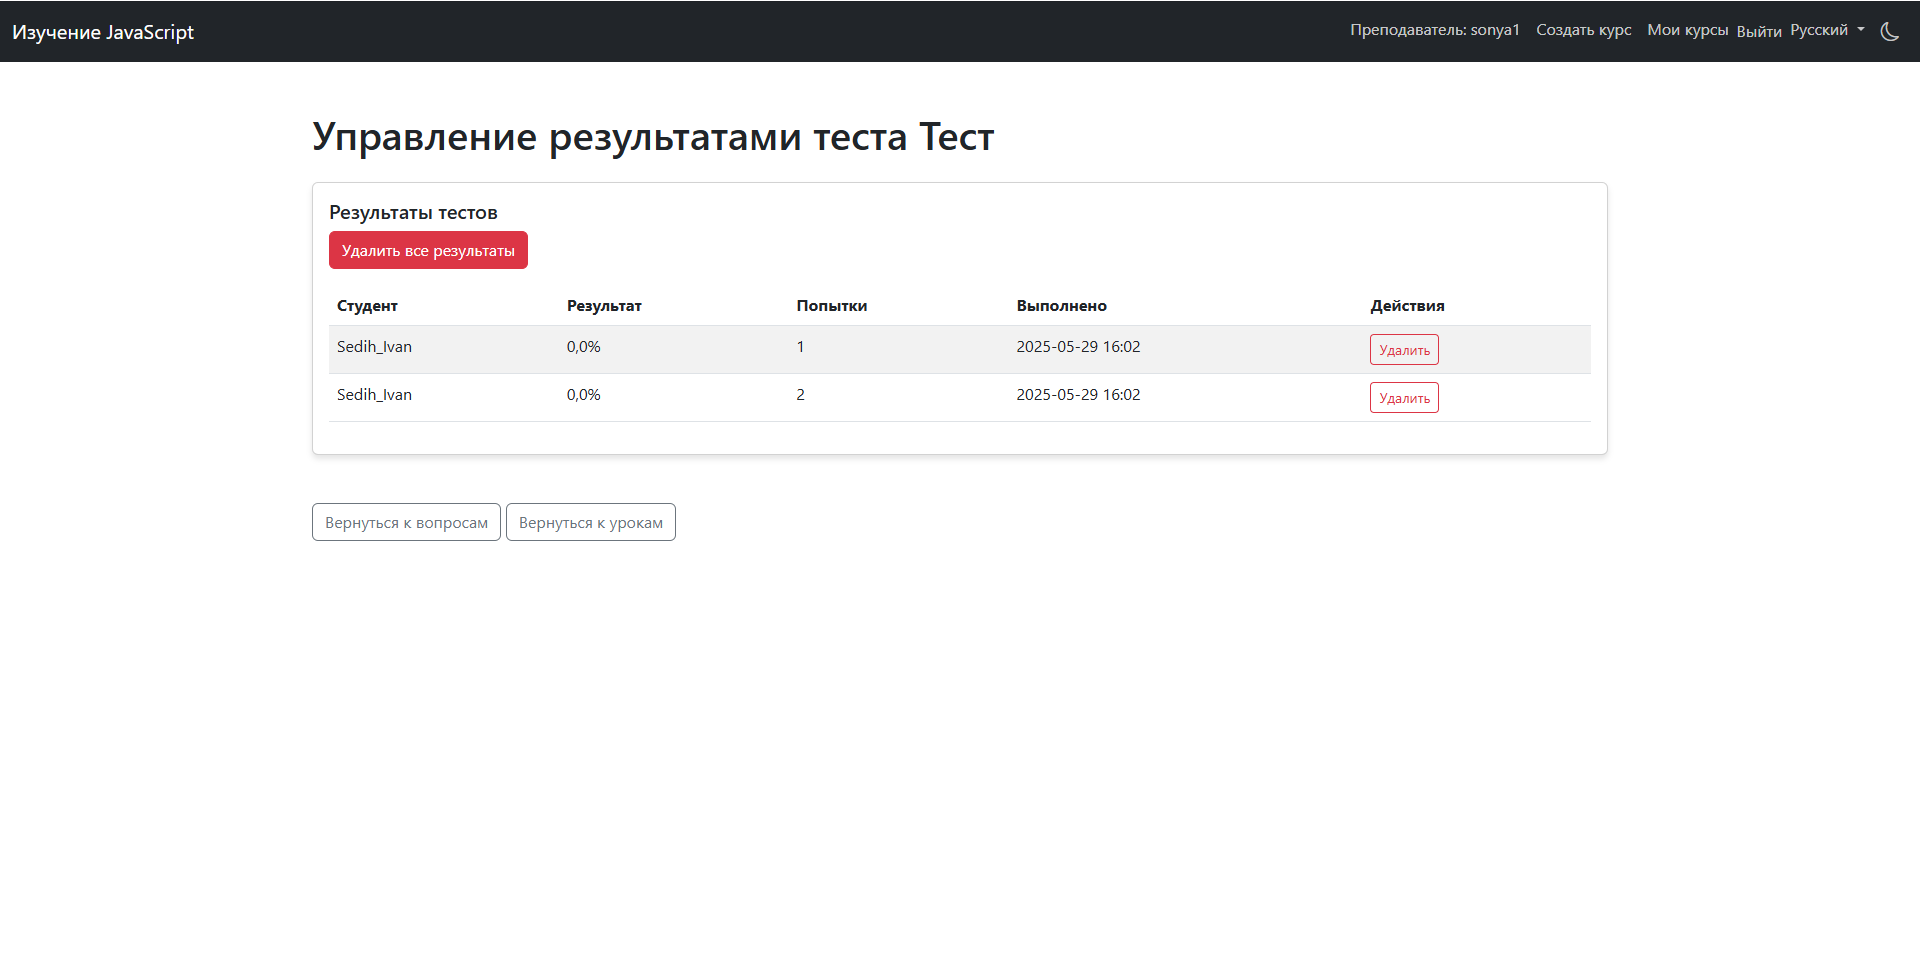
\includegraphics[width=1\linewidth]{images/резы} 
	\caption{Отчёт по результатам тестов}
	\label{zotchet:image}
\end{figure}

Ключевой особенностью данного отчёта является ограничение на количество попыток прохождения теста. Если студент превышает допустимое число попыток, доступ к тесту блокируется, и система уведомляет об этом (messages.error). Каждому отчёту присваивается уникальный идентификатор, исключающий дублирование данных при формировании статистики за определённый период.

Поскольку результаты тестов фиксируются в базе данных SQLite, отчёт не подлежит обнулению или повторному формированию без вмешательства администратора. Данные о результатах автоматически передаются преподавателю через интерфейс (managetestresults), что упрощает анализ. 

Отчёт по результатам тестов необходим: 

\begin{itemize}
	\item студенту для отслеживания своего прогресса и улучшения результатов; 
	\item преподавателю для контроля успеваемости и корректировки учебного плана; 
	\item администратору системы для анализа активности пользователей и проверки корректности работы модуля тестирования.
\end{itemize}

\subsection{Сравнительный анализ аналогичных систем}

Для оценки разработанной системы рассмотрим аналогичные платформы управления обучением, сравним их функциональность и определим конкурентные преимущества.

\subsubsection{Примеры аналогичных систем}

\begin{enumerate}
	\item Moodle --- популярная открытая LMS, используемая в образовательных учреждениях. Она поддерживает создание курсов, тестирование и управление пользователями через модульную архитектуру.
	\item Canvas LMS --- коммерческая LMS, ориентированная на образовательные учреждения и корпоративное обучение. Известна интуитивным интерфейсом и интеграцией с внешними инструментами (Google Drive, Zoom).
	\item Google Classroom --- бесплатная платформа от Google для упрощённого обучения. Интегрируется с экосистемой Google, но подходит скорее для школ и небольших групп.
\end{enumerate}

\subsubsection{Сравнение функциональности}

\begin{xltabular}{\textwidth}{|p{3.1cm}|p{3.1cm}|p{3.5cm}|X|}
	\caption{Сравнение функциональности систем управления обучением\label{comparison:table}}\\ \hline
	Функция & Система & Описание & Дополнительные замечания \\ \hline
	\endfirsthead
	\continuecaption{Продолжение таблицы \ref{comparison:table}}\\ \hline
	Функция & Система & Описание & Дополнительные замечания \\ \hline
	\endhead
	Управление курсами & Разработанная система & Создание курсов, запись студентов, отслеживание прогресса (courses\_enrol-lment). & Простая структура хранения. \\ \hline
	Управление курсами & Moodle & Курсы с категориями и ролями. & Сложная иерархия. \\ \hline
	Управление курсами & Canvas LMS & Гибкие настройки доступа, модули. & Интеграция с внешними инструментами. \\ \hline
	Управление курсами & Google Classroom & Быстрое создание курсов, минимум опций. & Только базовые функции. \\ \hline
	
	Управление уроками & Разработанная система & Добавление уроков, сортировка по полю (order), прогресс через (courses\_prog-ress). & Контроль доступности. \\ \hline
	Управление уроками & Moodle & Уроки с медиа и интерактивом. & Широкий функционал. \\ \hline
	Управление уроками & Canvas LMS & Модульная структура, поддержка мультимедиа. & Гибкая система. \\ \hline
	Управление уроками & Google Classroom & Уроки как задания. & Ограниченная настройка. \\ \hline
	
	Управление тестами & Разработанная система & Создание тестов, локализация, подсчёт баллов (courses\_test, courses\_question). & Поддержка разных языков. \\ \hline
	Управление тестами & Moodle & Типы вопросов, разветвлённая аналитика. & Гибкая система оценивания. \\ \hline
	Управление тестами & Canvas LMS & Автоматизация и интеграции. & Расширенные возможности. \\ \hline
	Управление тестами & Google Classroom & Тесты через Google Forms. & Простой интерфейс. \\ \hline
	
	Аналитика и результаты & Разработанная система & Отчёты: средний, макс./мин. баллы (courses\_test-result). & Основной набор аналитики. \\ \hline
	Аналитика и результаты & Moodle & Расширенные отчёты, экспорт, группировка. & Удобно для ВУЗов. \\ \hline
	Аналитика и результаты & Canvas LMS & Визуализация результатов. & Графики, интерактивность. \\ \hline
	Аналитика и результаты & Google Classroom & Базовая статистика. & Ограниченный функционал. \\ \hline
	
	Локализация & Разработанная система & Интерфейс и контент через Django i18n. & Многоязычная поддержка. \\ \hline
	Локализация & Moodle & Поддержка языков через плагины. & Требует настройки. \\ \hline
	Локализация & Canvas LMS & Интерфейс локализован, контент частично. & Неполная поддержка. \\ \hline
	Локализация & Google Classroom & Интерфейс от Google, контент не локализуется. & Только интерфейс. \\ \hline
	
	Поддержка пользователей & Разработанная система & Регистрация, роли (isteacher, isstudent), доступ через (login\_required). & Простая авторизация. \\ \hline
	Поддержка пользователей & Moodle & Пользователи, группы, LDAP. & Подходит для больших структур. \\ \hline
	Поддержка пользователей & Canvas LMS & SSO, управление пользователями. & Высокая безопасность. \\ \hline
	Поддержка пользователей & Google Classroom & Аккаунты Google, базовые роли. & Простое управление. \\ \hline
\end{xltabular}




\subsubsection{Сравнительный анализ}

{Управление курсами и уроками.} Разработанная система обеспечивает базовые функции управления курсами и уроками с автоматическим контролем доступа, что подходит для самостоятельного обучения. Moodle и Canvas предлагают более сложные инструменты (категории, модули), но их сложность может быть избыточной для разработанной платформы. Google Classroom проще, но не поддерживает зависимости между уроками.

{Управление тестами.} Разработанная система выделяется локализацией вопросов и ответов, что важно для иностранной аудитории. Moodle и Canvas поддерживают больше типов вопросов (например, эссе), но требуют больше времени на настройку. Google Classroom ограничен Google Forms, что менее гибко.

{Аналитика.} Разработанная система предоставляет базовые отчёты, достаточные для небольшой платформы. Moodle и Canvas предлагают более мощную аналитику (графики, экспорт), но это может быть избыточным. Google Classroom уступает по аналитическим возможностям.

{Локализация.} Локализация через Django i18n делает разработанную систему удобной для пользователей с разными языками, особенно в части вопросов тестов. Moodle требует дополнительных пакетов для переводов, а Canvas и Google Classroom ограничены локализацией интерфейса.

{Поддержка пользователей.} Разработанная система использует Django contrib.auth для базовой аутентификации. Moodle и Canvas предлагают сложные механизмы (SSO, LDAP), которые могут быть избыточными. Google Classroom ограничивается Google Accounts.

\subsubsection{Преимущества и недостатки разработанной системы}

{Преимущества:}
\begin{itemize}
	\item локализация вопросов и ответов тестов через Django i18n;
	\item простота управления уроками с автоматическим доступом по прогрессу;
	\item лёгкая интеграция с SQLite для хранения и аналитики данных;
	\item простая и интуитивная система управления пользователями.
\end{itemize}

{Недостатки:}
\begin{itemize}
	\item ограниченные аналитические возможности (нет графиков, экспорта данных);
	\item отсутствие поддержки сложных типов вопросов (например, эссе);
	\item нет интеграции с внешними инструментами (например, Zoom, Google Drive).
\end{itemize}

\subsubsection{Выводы}

Разработанная система эффективно решает задачи управления обучением, предлагая удобный интерфейс, локализацию и автоматизацию. Для конкуренции с Moodle или Canvas можно добавить расширенную аналитику и поддержку сложных типов вопросов. Google Classroom уступает в гибкости, что делает разработанную платформу более подходящей для узкоспециализированных образовательных задач.




\section{Техническое задание}
\subsection{Основание для разработки}

Основанием для разработки является задание на выпускную квалификационную работу бакалавра "<Веб-приложение для компьютерной поддержки самостоятельной работы  иностранных студентов при изучении языка программирования  JavaScript">.

\subsection{Цель и назначение разработки}

Основной задачей выпускной квалификационной работы является разработка и внедрение веб-приложения для компьютерной поддержки самостоятельной работы  иностранных студентов при изучении языка программирования  JavaScript.

Посредством внедрения веб-приложения планируется устранить существующие недостатки, связанные с неструктурированным доступом к учебным материалам, отсутствием интерактивных инструментов для практики и тестирования, а также сложностями в организации учебного процесса для иностранных студентов, включая языковые барьеры.

Цель разработки включает следующие подцели:

\begin{itemize}
\item создание единой образовательной платформы для доступа к учебным курсам, урокам и тестам;
\item обеспечение удобного и интуитивно понятного интерфейса для самостоятельного изучения JavaScript;
\item интеграция инструментов для проверки знаний, таких как тесты с автоматической оценкой;
\item оптимизация процессов управления учебным контентом для преподавателей и взаимодействия студентов с платформой.
\end{itemize}

\subsection{Функциональные задачи}

Разрабатываемая веб-платформа включает в себя следующие модули:
\begin{enumerate}
\item {Курсы} — модуль для создания и управления учебными курсами, включающими уроки и тесты. Преподаватели могут добавлять, редактировать и удалять курсы, а студенты получают доступ к материалам.
\item {Уроки} — система управления учебным контентом, позволяющая структурировать материалы курса (текст, изображения, видео) и задавать порядок уроков. Поддерживается предпросмотр уроков и их редактирование.
\item {Тесты} — модуль для создания и прохождения интерактивных тестов. Преподаватели могут задавать вопросы и варианты ответов, а студенты проходят тесты с автоматической оценкой результатов.
\item {Результаты тестов} — инструмент для анализа успеваемости студентов. Преподаватели могут просматривать, удалять и управлять результатами тестов, включая статистику по студентам.
\item {Панель управления преподавателя} — интерфейс для управления курсами, уроками, тестами и результатами, с удобной навигацией и виджетами для быстрого доступа.
\item {Профиль пользователя} — модуль для управления учетной записью, включая настройки аватара и персональной информации.
\item {Сообщения} — система уведомлений для обратной связи (например, сообщения об успешном добавлении урока или удалении результатов).
\item {Панель управления} — страница с виджетами всех вышеперечисленных сервисов.
\end{enumerate}

\subsection{Требования пользователя к интерфейсу web-сайта}

Платформа должна обеспечивать:
\begin{itemize}
    \item авторизацию;
    \item интуитивно понятную навигацию между модулями;
    \item адаптивный интерфейс для десктопных и мобильных устройств.
\end{itemize}

Композиция интерфейса пользователя представлена на рисунках ~\ref{templ:image1}, ~\ref{templ:image2}, ~\ref{templ:image3}, ~\ref{templ:image4}, ~\ref{templ:image5}, ~\ref{templ:image6}, ~\ref{templ:image7}, ~\ref{templ:image8}, ~\ref{templ:image9},  ~\ref{templ:image10}.
\newpage  

Композиция шаблона курсы представлена на рисунке ~\ref{templ:image1} и состоит из:

\begin{itemize}
	\item кнопка для просмотра курса (1);
	\item окна с информацией роли профиля и имени (2);
	\item кнопка для создания курса (3);
	\item кнопка для просмотра своих курсов (4);
	\item кнопка для выхода (5);
	\item кнопка для смены языка (6).
\end{itemize}

\begin{figure}[h]
	\centering
	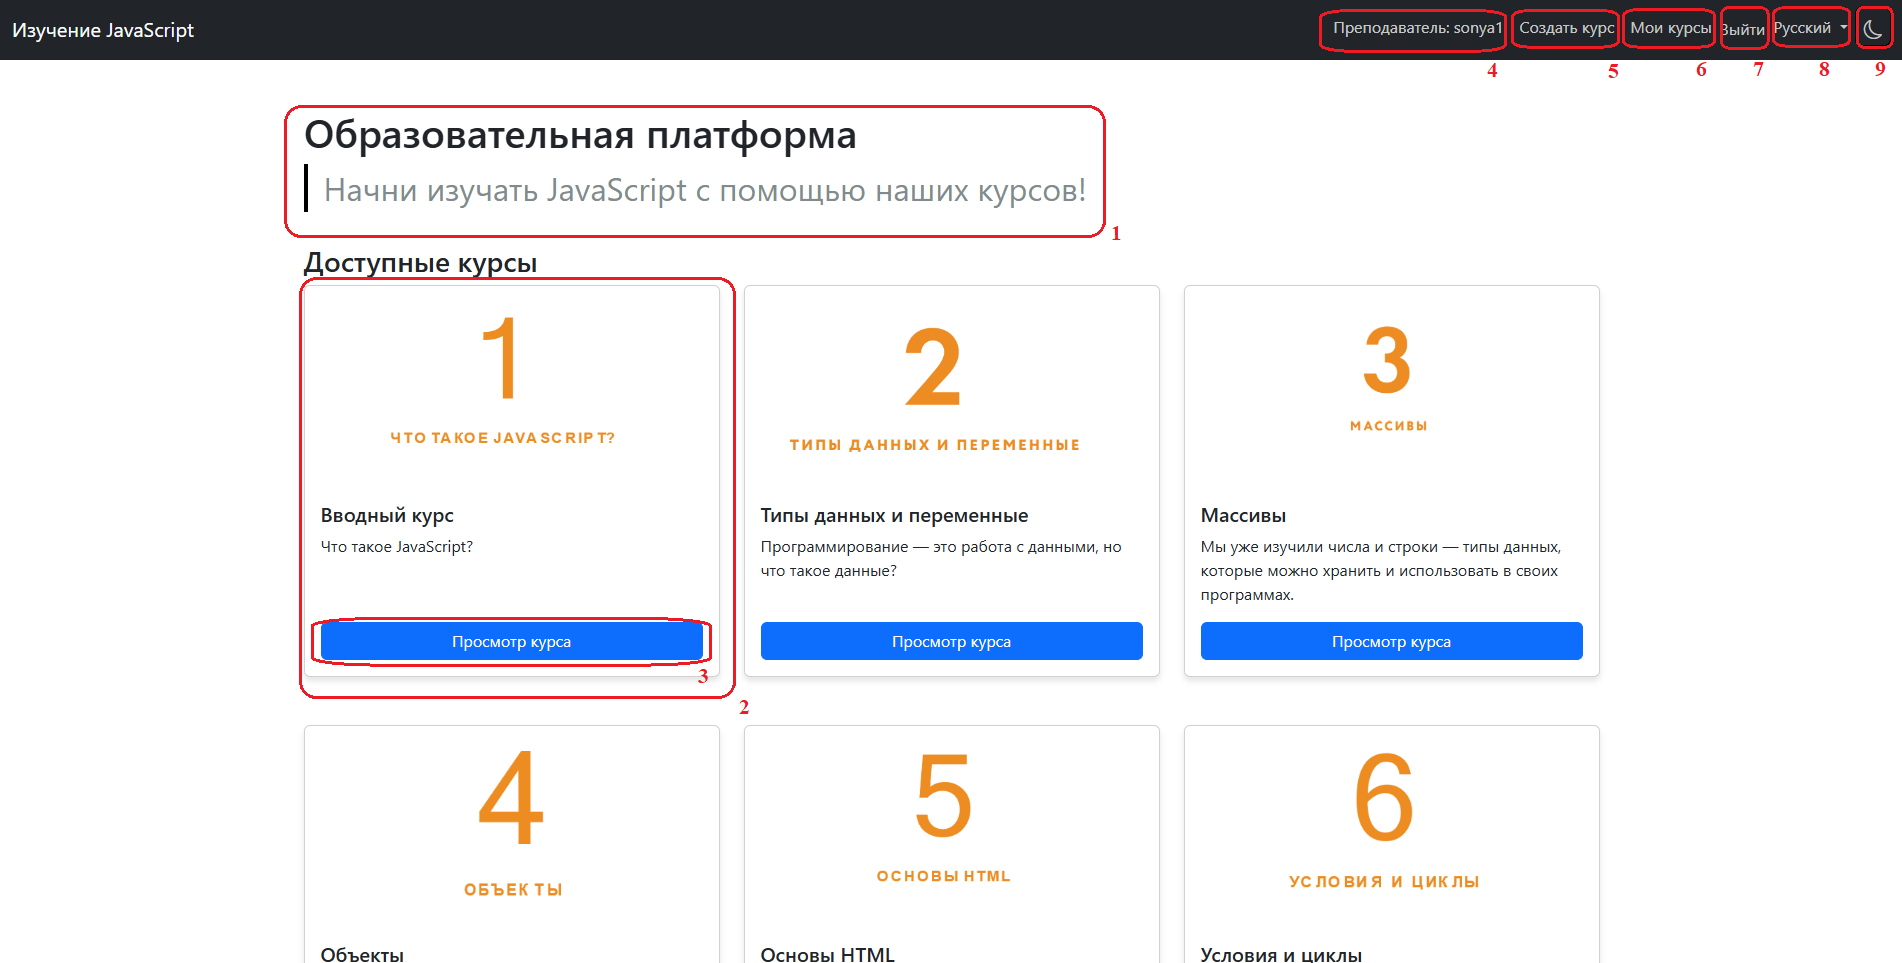
\includegraphics[width=1\linewidth]{images/курсы}
	\caption{Композиция интерфейса сервиса <<Курсы>>}
	\label{templ:image1}
\end{figure}

Композиция шаблона панель управления преподавателя представлена на рисунке ~\ref{templ:image2} и состоит из:

\begin{itemize}
	\item кнопка для редактирования курса (1);
	\item кнопка для управления уроками (2);
	\item кнопка для просмотра курса (3);
	\item кнопка для удаления курса (4).
\end{itemize}

\begin{figure}[h]
	\centering
	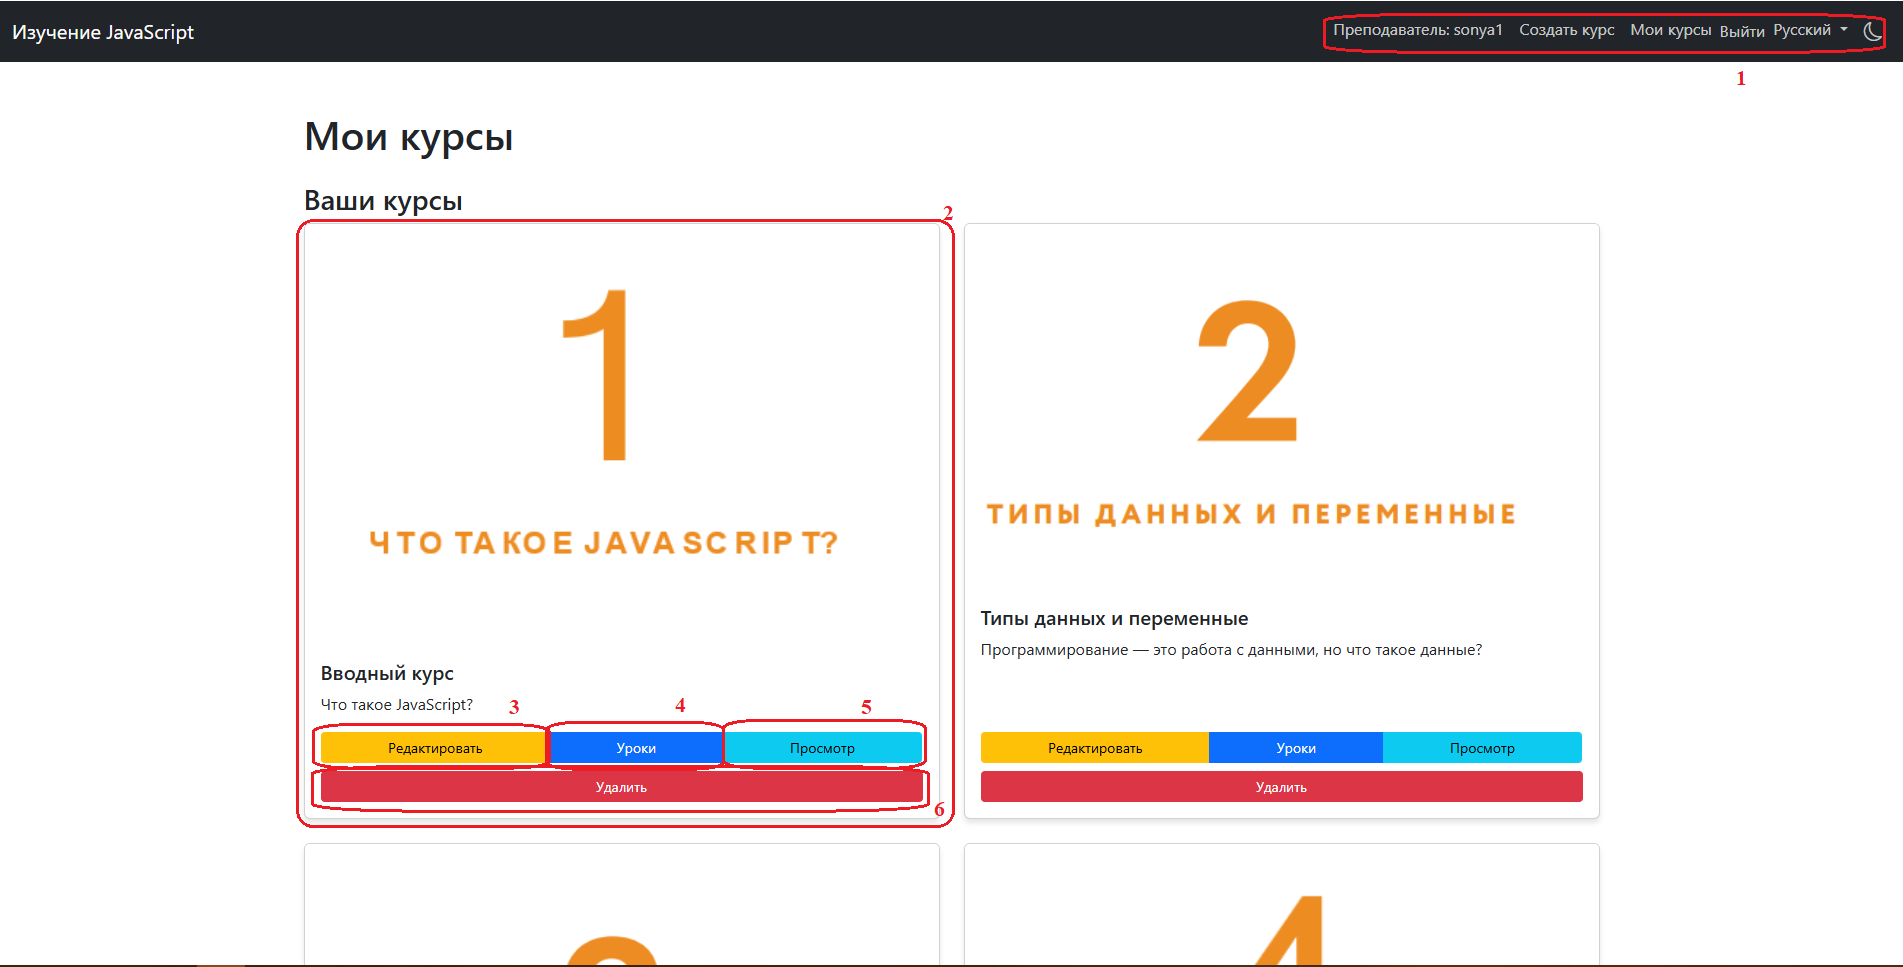
\includegraphics[width=1\linewidth]{images/учитель}
	\caption{Композиция интерфейса сервиса <<Панель управления преподавателя>>}
	\label{templ:image2}
\end{figure}
\newpage 

Композиция шаблона уроки представлена на рисунке ~\ref{templ:image3} и состоит из:

\begin{itemize}
	\item кнопка для просмотра урока (1);
	\item окна курса (2);
	\item окно уроков (3);
	\item навигационная панель (4).
\end{itemize}

\begin{figure}[h]
	\centering
	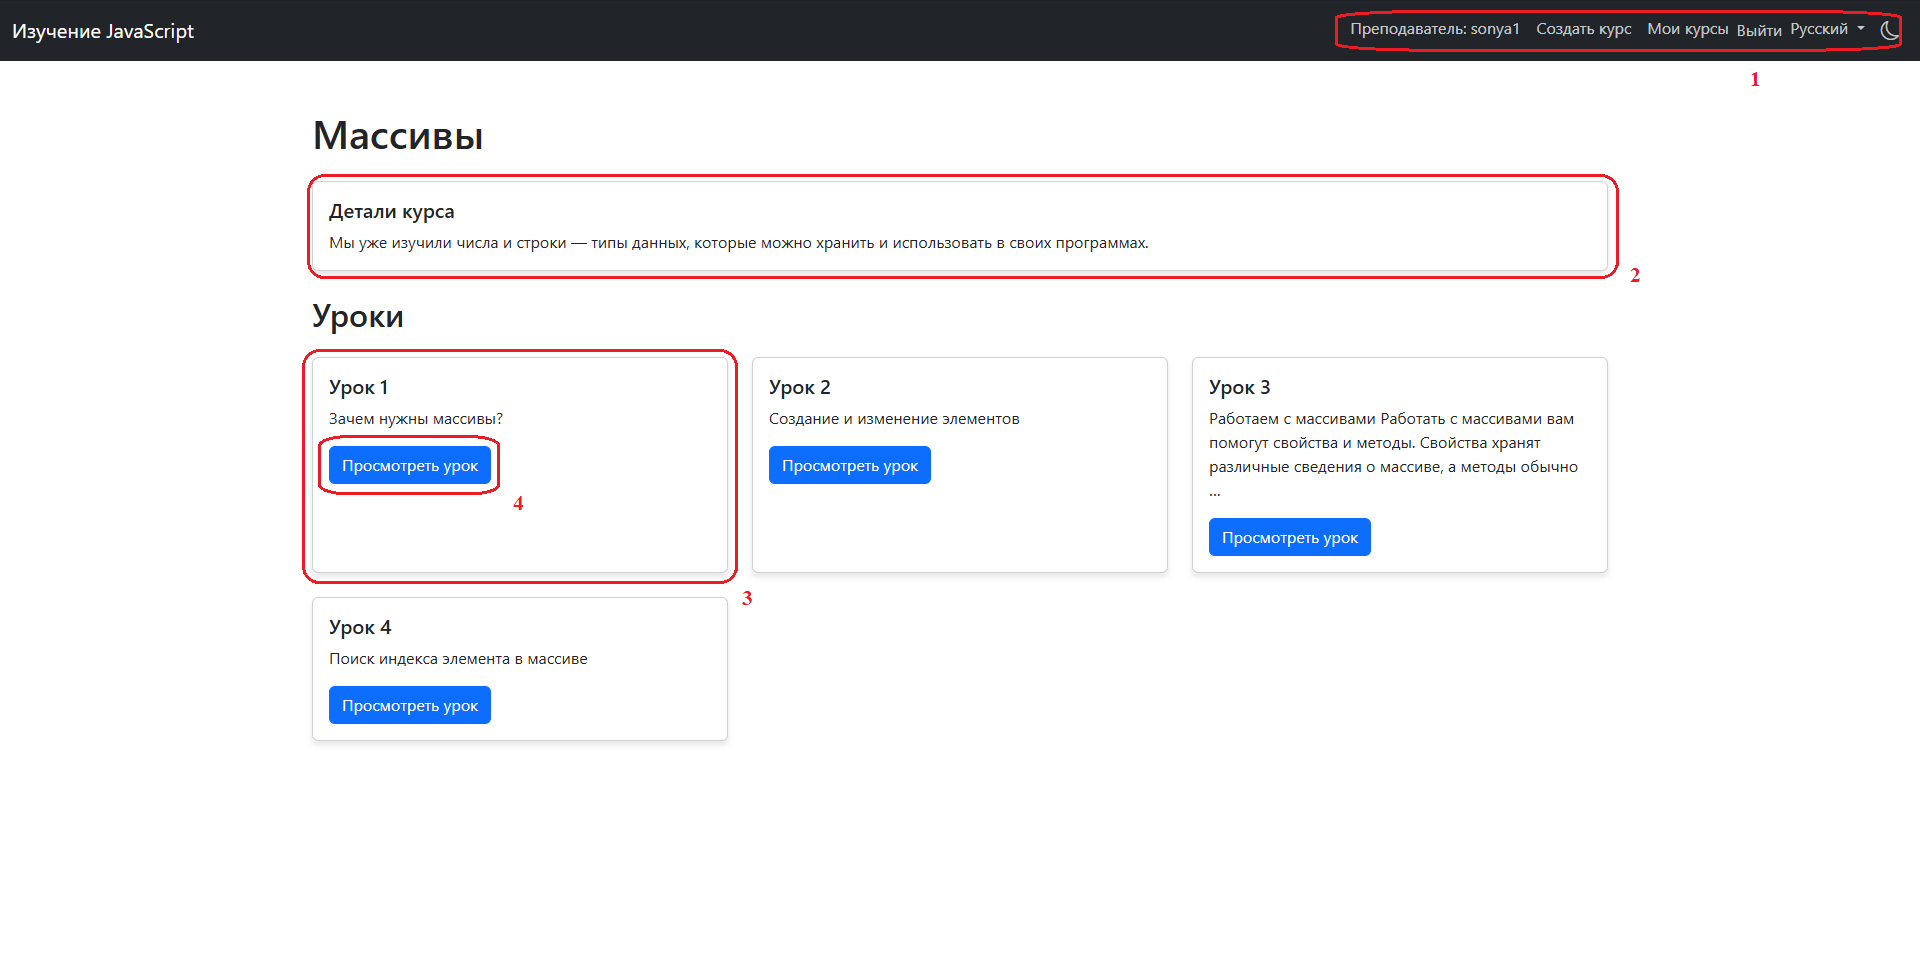
\includegraphics[width=1\linewidth]{images/уроки}
	\caption{Композиция интерфейса сервиса <<Уроки>>}
	\label{templ:image3}
\end{figure}

Композиция шаблона тесты представлена на рисунке ~\ref{templ:image4} и состоит из:

\begin{itemize}
	\item окно уроков (1);
	\item кнопка редактировать урок (2);
	\item кнопка просмотр урока (3);
	\item кнопка обложка урока (4);
	\item кнопка добавить тест (5);
	\item кнопка управление вопросами (6);
	\item кнопка управление результатами (7).
\end{itemize}

\begin{figure}[h]
	\centering
	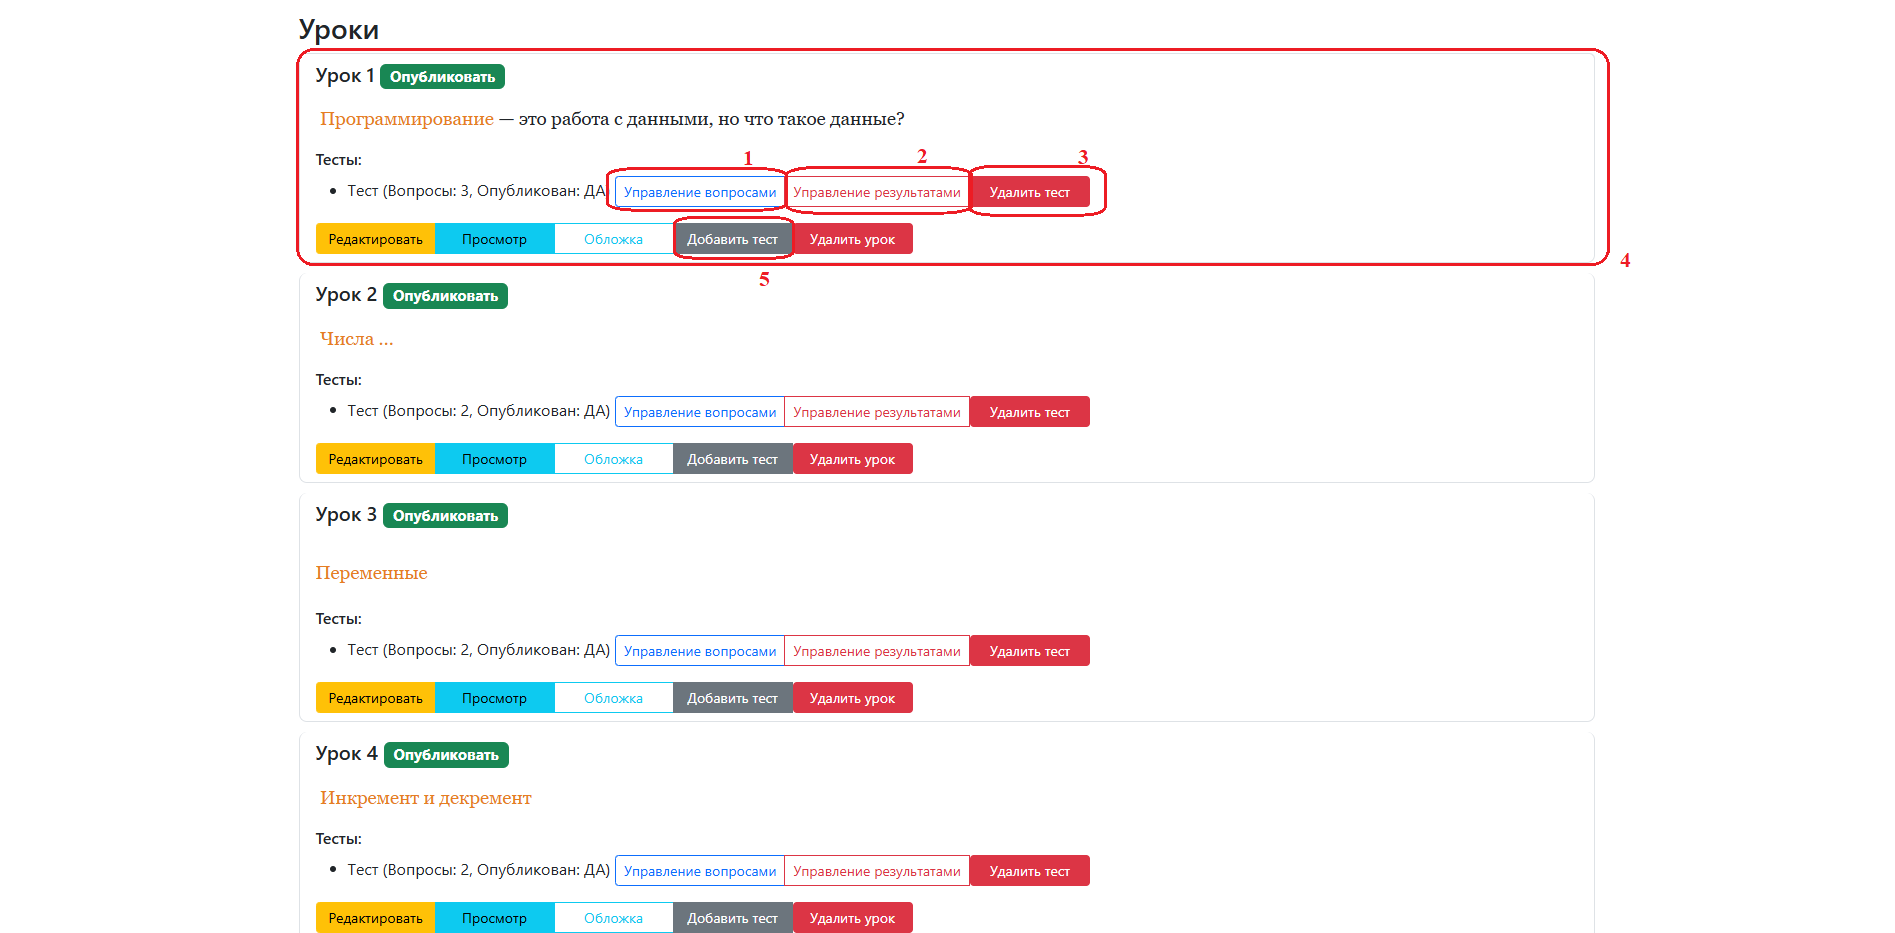
\includegraphics[width=1\linewidth]{images/Тесты}
	\caption{Композиция интерфейса сервиса <<Тесты>>}
	\label{templ:image4}
\end{figure}

Композиция шаблона создание теста представлена на рисунке ~\ref{templ:image5} и состоит из:

\begin{itemize}
	\item окно создания теста (1);
	\item поле ввода заголовка теста (2);
	\item поле ввода описания теста (3);
	\item поле ввода минимального балла (4);
	\item поле выбора статуса (5);
	\item кнопка для создания теста (6);
	\item кнопка возвращения к уроку (7).
\end{itemize}

\begin{figure}[h]
	\centering
	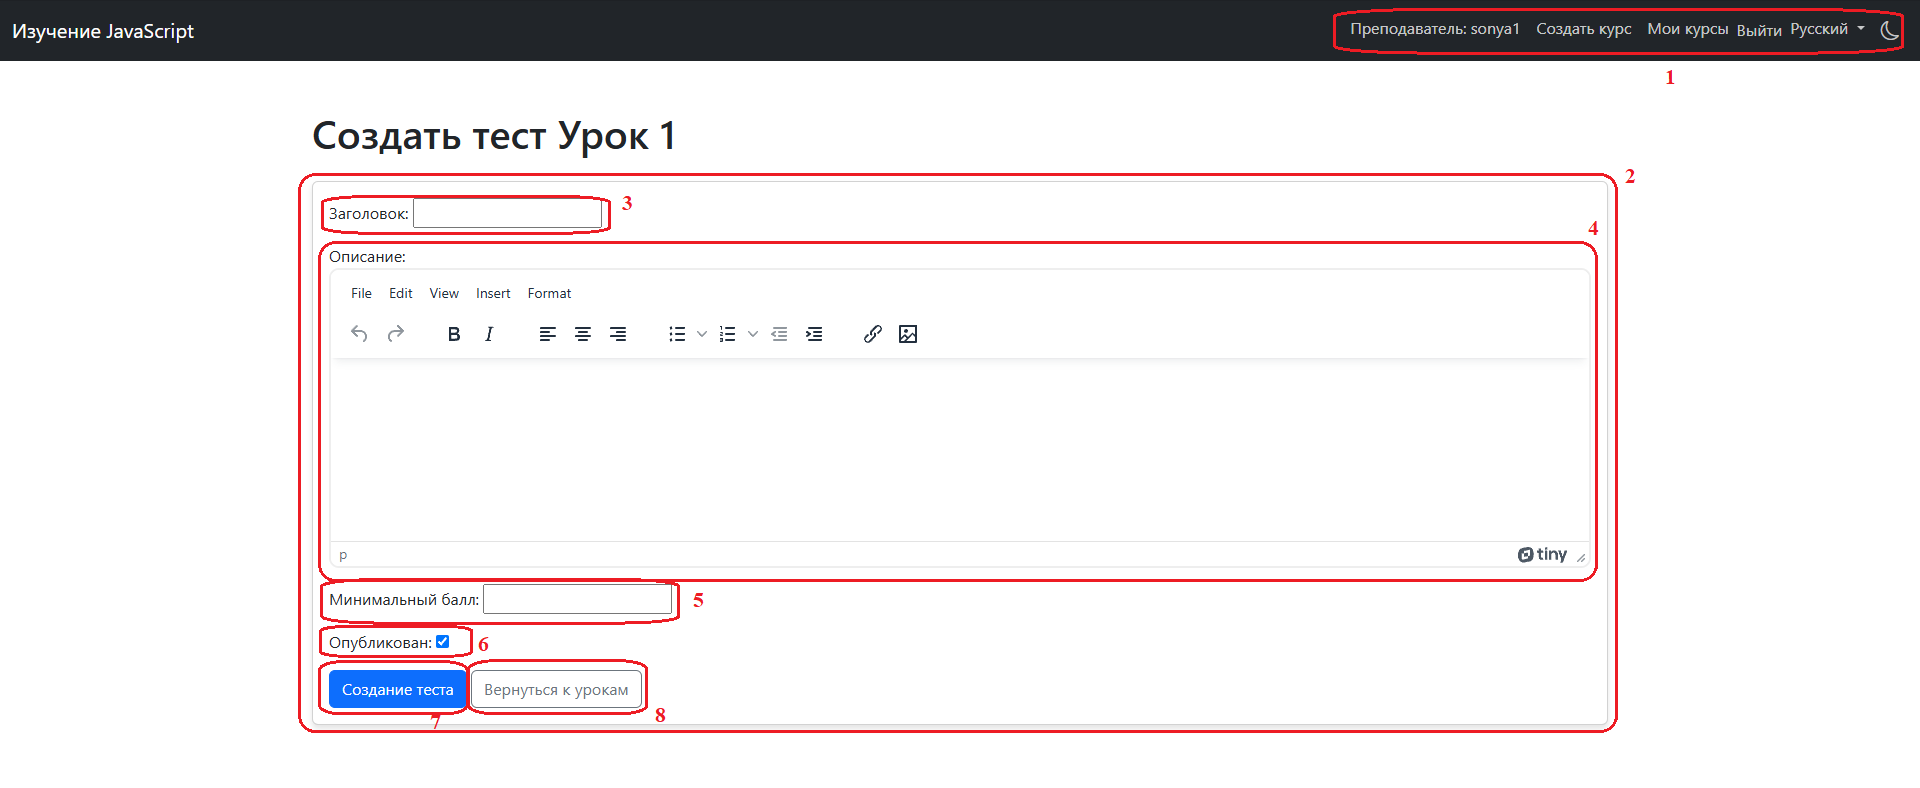
\includegraphics[width=1\linewidth]{images/создатьтест}
	\caption{Композиция интерфейса сервиса <<Создание теста>>}
	\label{templ:image5}
\end{figure}
\newpage

Композиция шаблона результаты теста представлена на рисунке ~\ref{templ:image6} и состоит из:

\begin{itemize}
	\item окна управления результатами теста (1);
	\item окна с результатами студентов  (2);
	\item кнопка удалить все результаты (3);
	\item кнопка удалить результат (4);
	\item кнопка вернуться к вопросам (5);
	\item кнопка вернуться к урокам (6).
\end{itemize}

\begin{figure}[h]
	\centering
	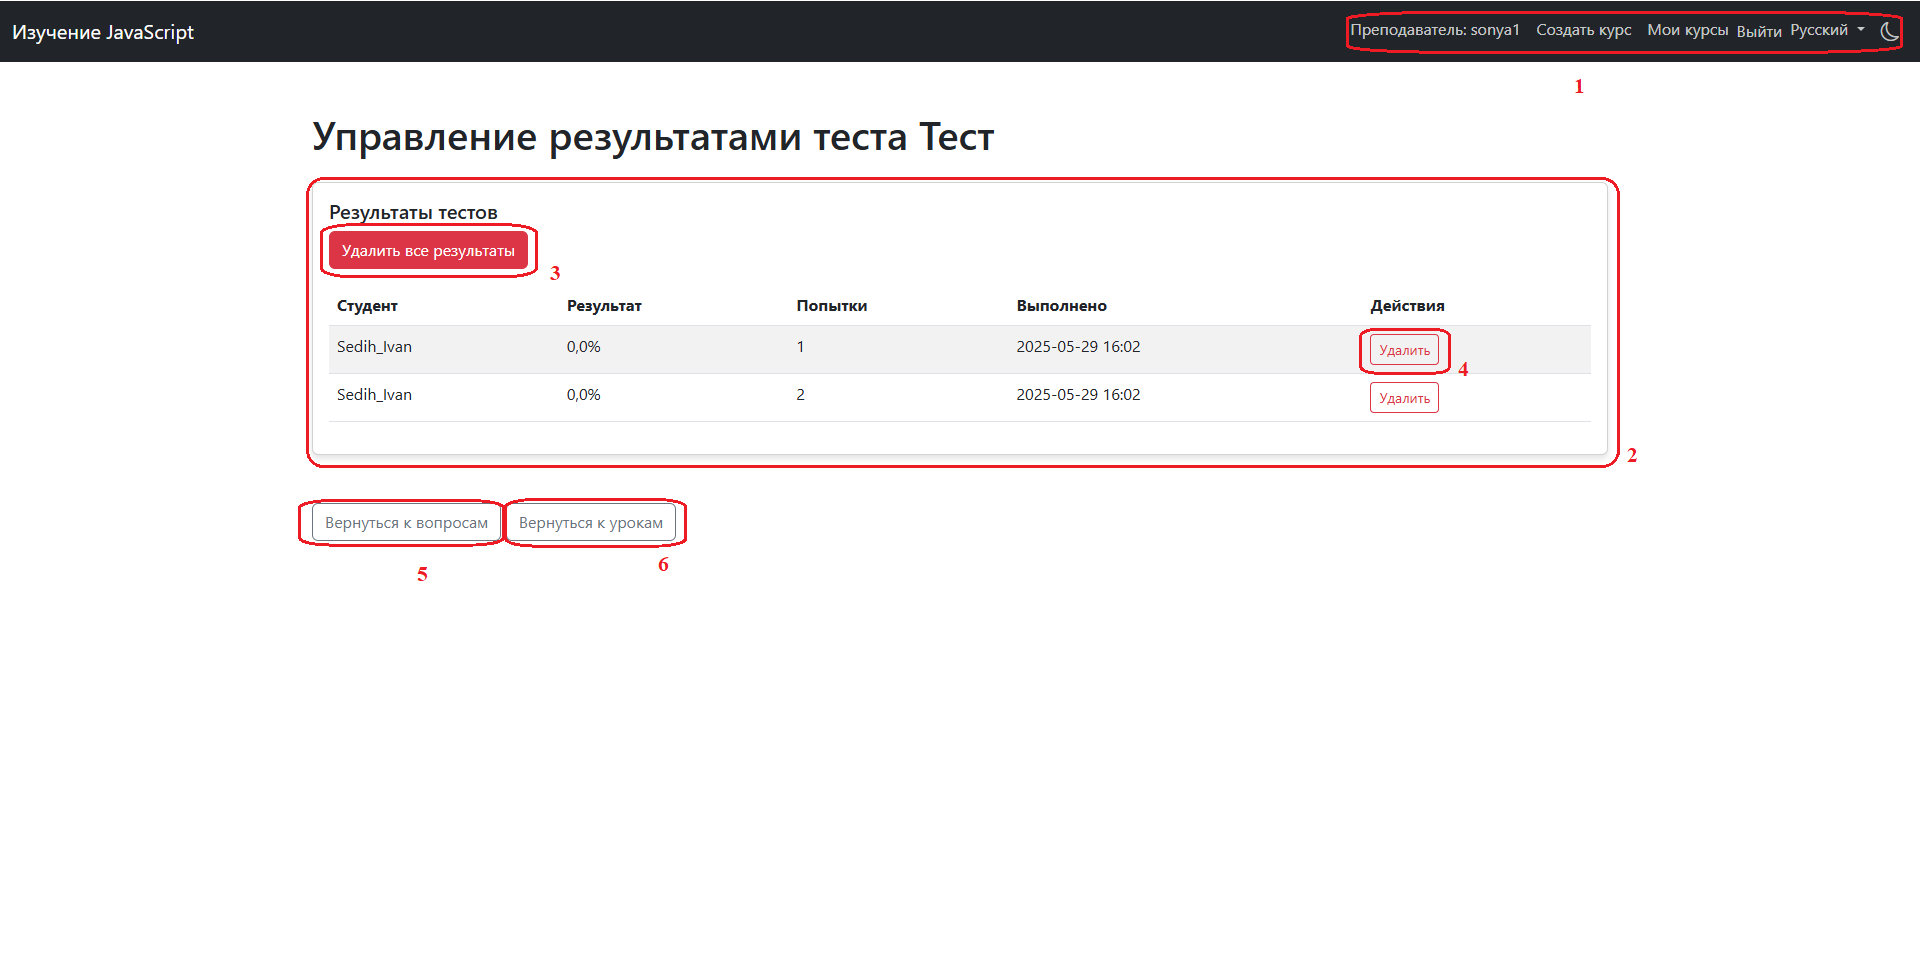
\includegraphics[width=1\linewidth]{images/результаты}
	\caption{Композиция интерфейса сервиса <<Результаты тестов>>}
	\label{templ:image6}
\end{figure}
\newpage
Композиция шаблона окна авторизации представлена на рисунке ~\ref{templ:image7} и состоит из:

\begin{itemize}
	\item поле для ввода кода (1);
	\item экранная клавиатура (2);
	\item кнопка для очистки поля (3);
	\item кнопка для подтверждения ввода пароля (4).
\end{itemize}

\begin{figure}[h]
	\centering
	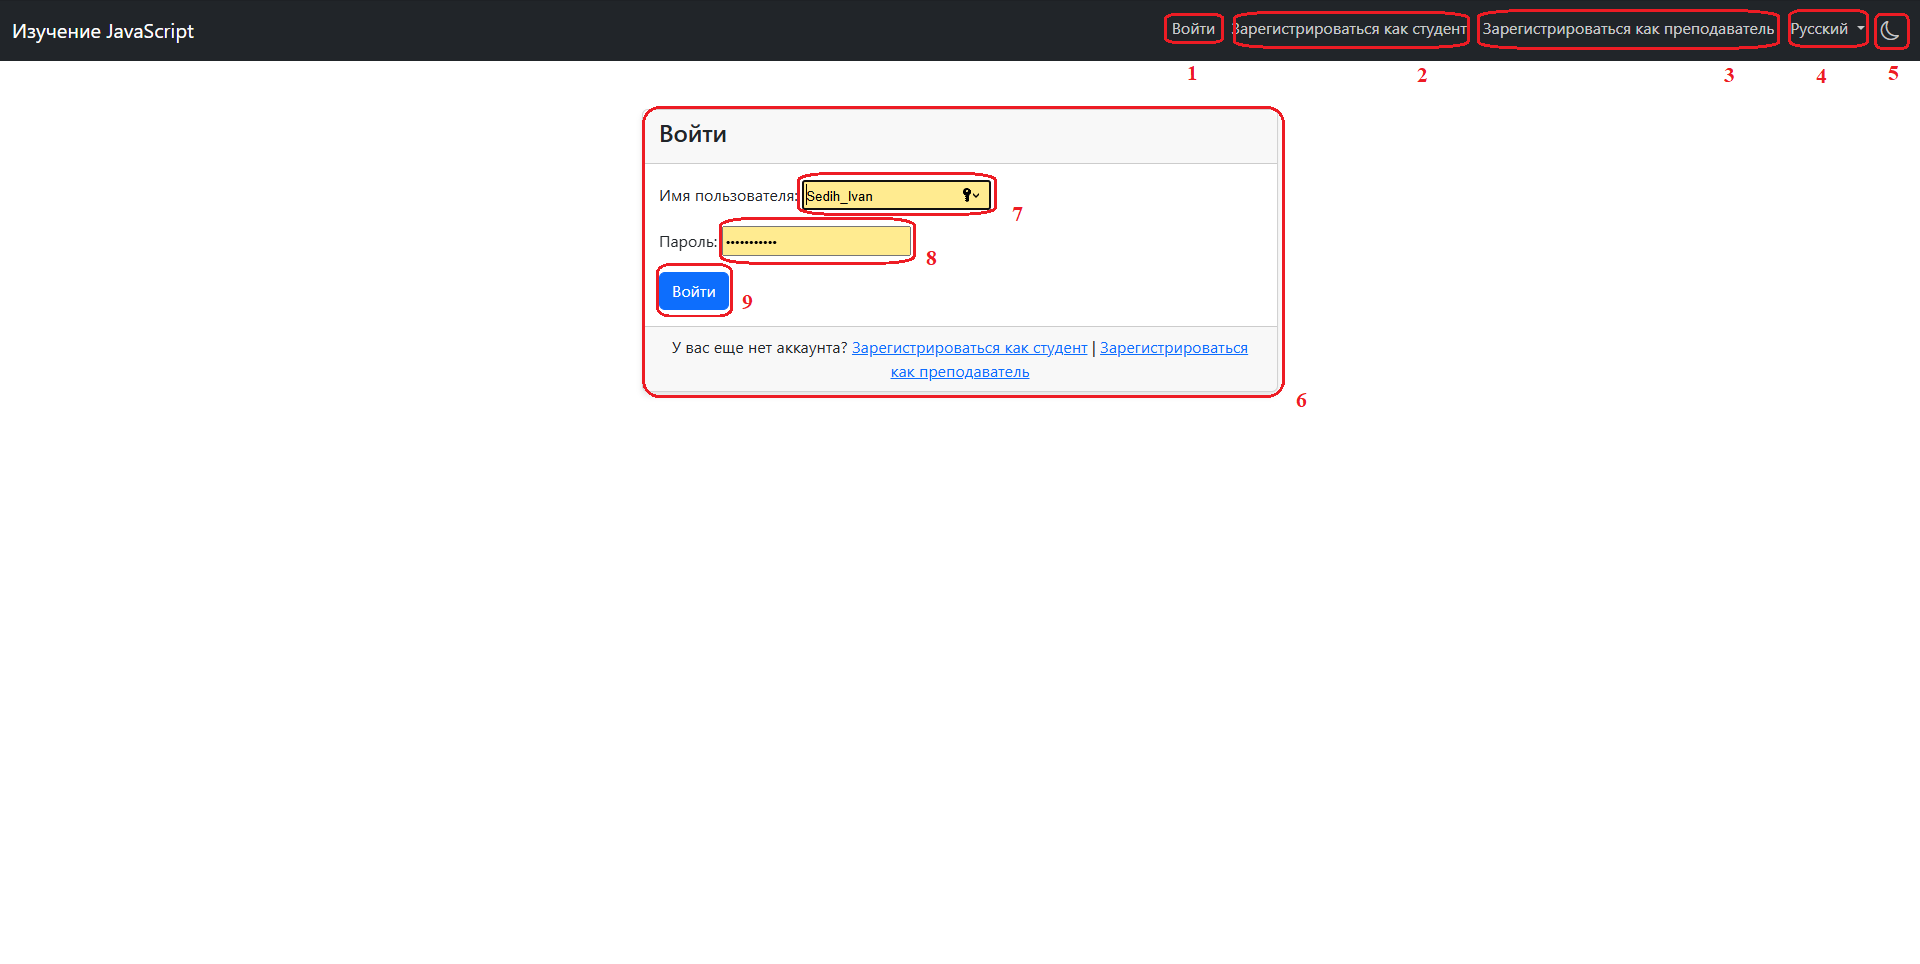
\includegraphics[width=1\linewidth]{images/Авторизация}
	\caption{Композиция интерфейса сервиса <<Авторизация>>}
	\label{templ:image7}
\end{figure}

Композиция шаблона профиль представлена на рисунке ~\ref{templ:image8} и состоит из:

\begin{itemize}
	\item окно курсов на которые записан (1);
	\item кнопка просмотра курса (2);
	\item кнопка отписаться (3).
\end{itemize}

\begin{figure}[h]
	\centering
	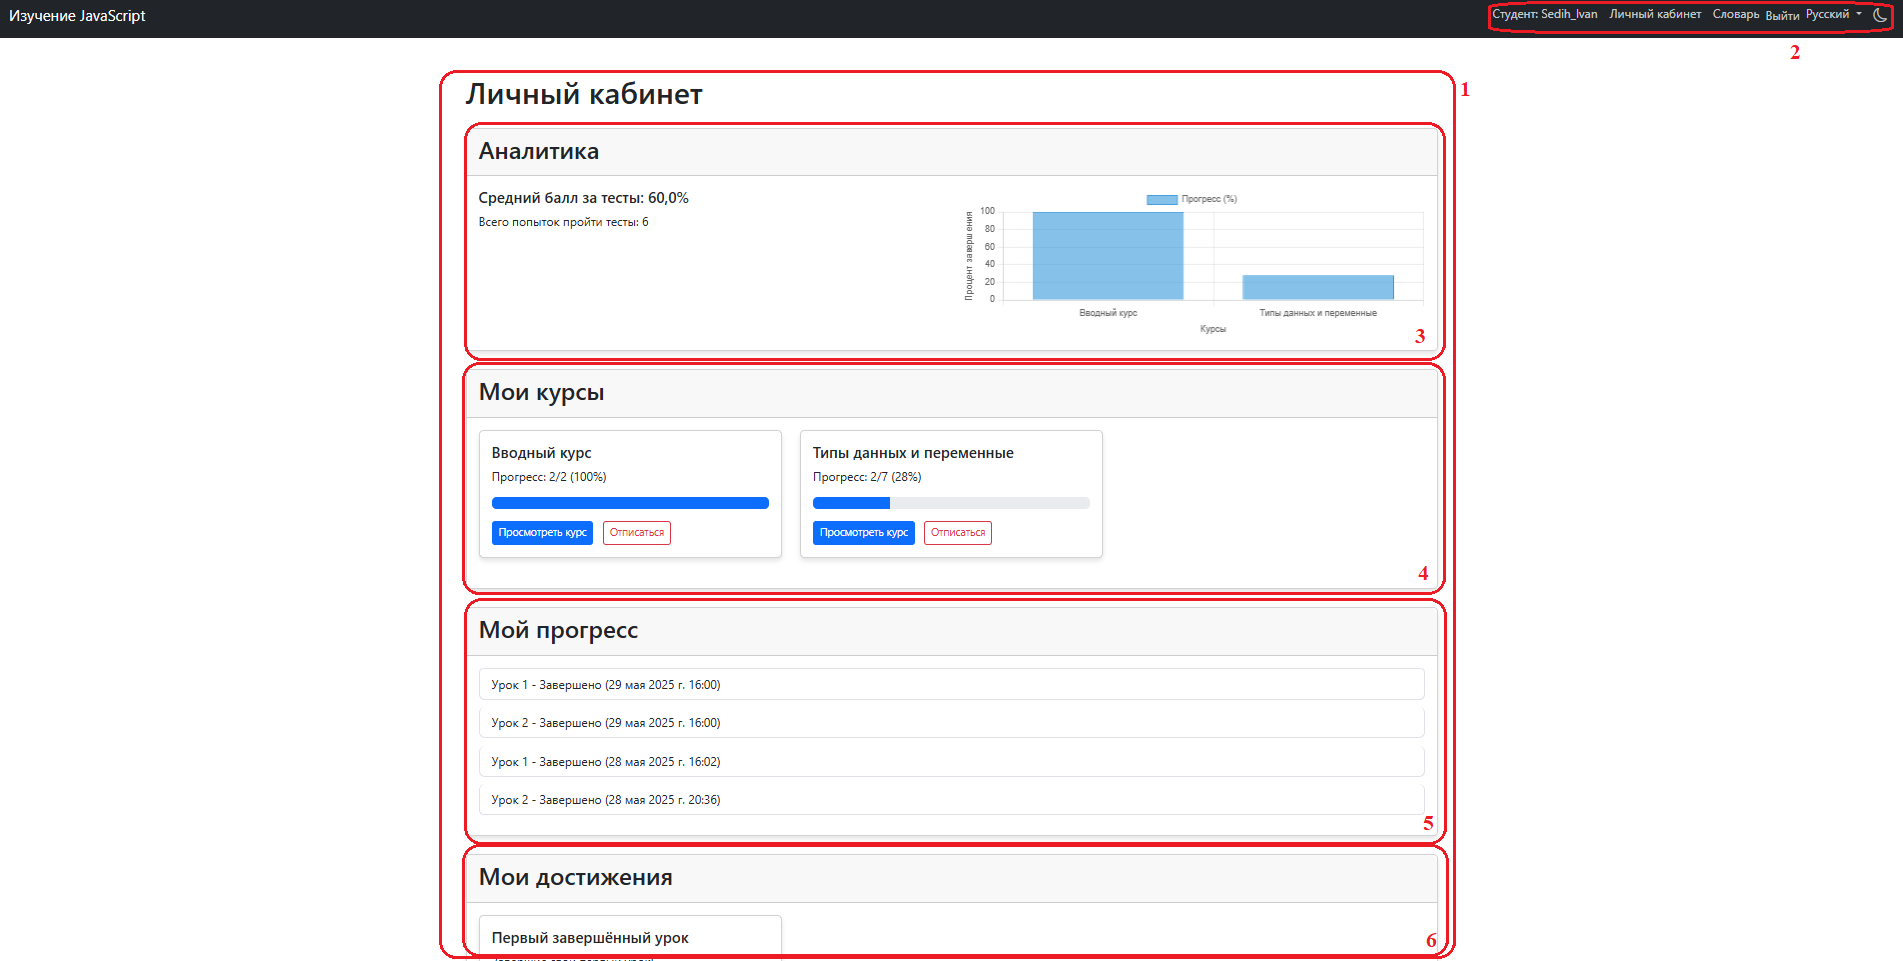
\includegraphics[width=1\linewidth]{images/профиль}
	\caption{Композиция интерфейса сервиса <<Профиль>>}
	\label{templ:image8}
\end{figure}


Композиция шаблона создание курса представлена на рисунке ~\ref{templ:image9} и состоит из:

\begin{itemize}
	\item окно создания курса (1);
	\item поле ввода заголовка курса (2);
	\item поле ввода описания курса (3);
	\item кнопка выбора изображения (4);
	\item поле выбора статуса курса (5);
	\item кнопка сохранения курса (6);
	\item кнопка отмены создания курса (7).
\end{itemize}

\begin{figure}[h]
	\centering
	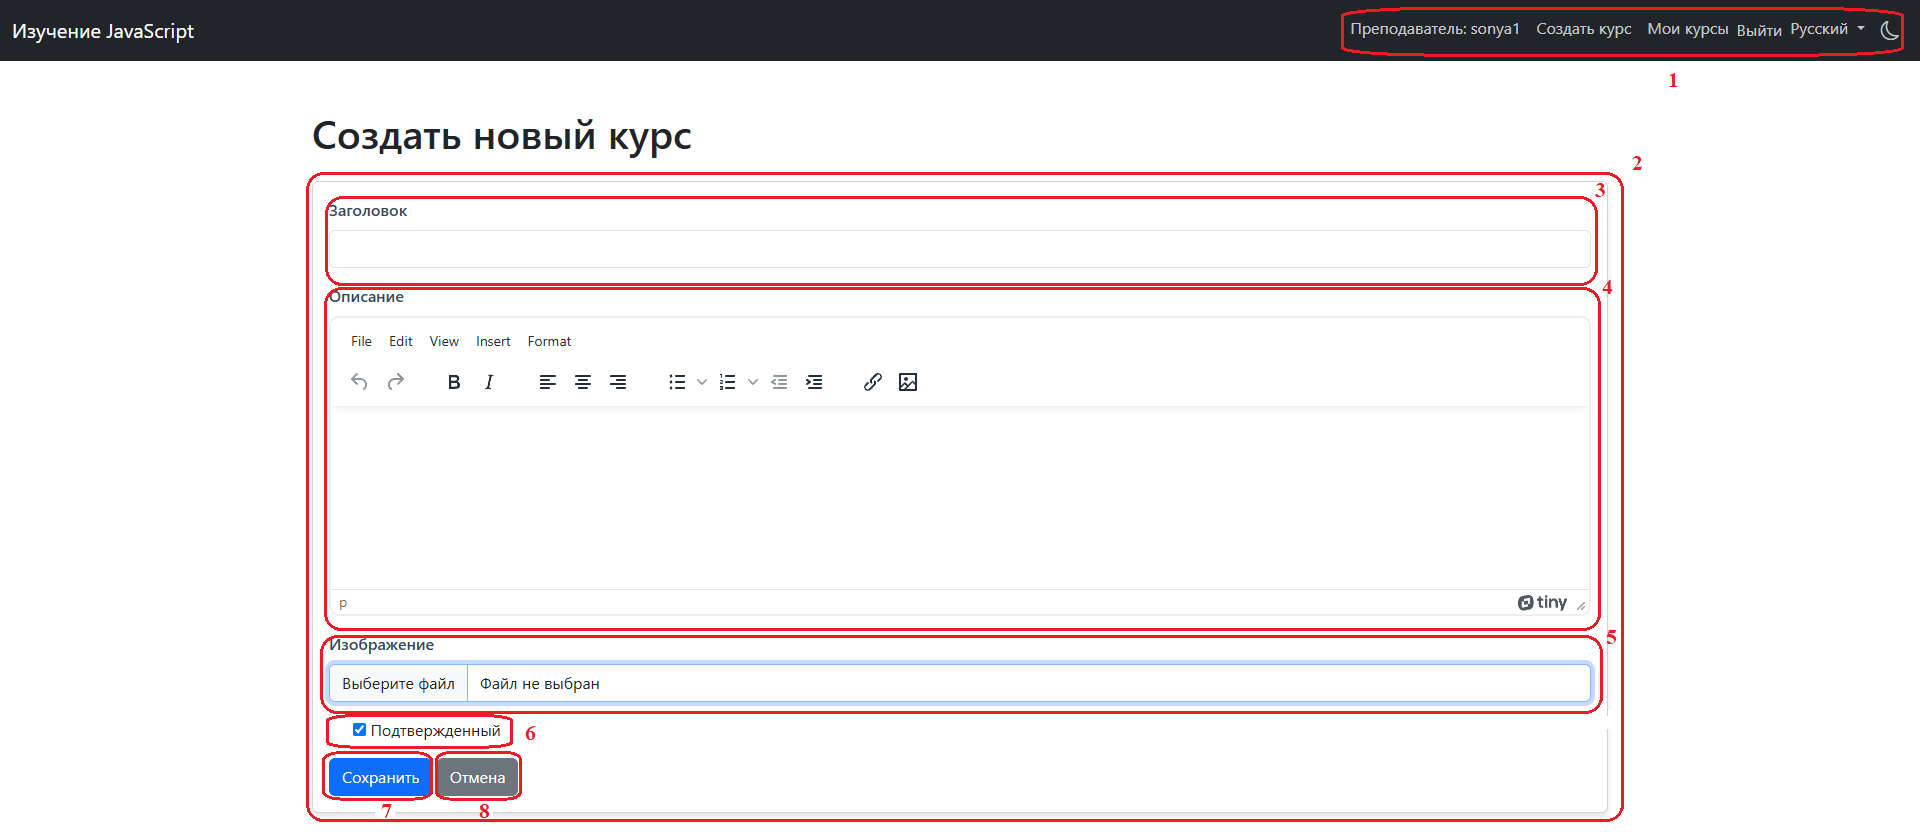
\includegraphics[width=0.9\linewidth]{images/создатькурс}
	\caption{Композиция интерфейса сервиса <<Создание курса>>}
	\label{templ:image9}
\end{figure}

\newpage
Композиция шаблона создание урока представлена на рисунке ~\ref{templ:image10} и состоит из:

\begin{itemize}
	\item окно создания урока (1);
	\item поле ввода заголовка урока (2);
	\item поле ввода описания урока (3);
	\item поле ввода материалов урока (4);
	\item поле ввода ссылки на видеоролик (5);
	\item поле выбора статуса урока (6);
	\item кнопка добавления урока (7).
\end{itemize}

\begin{figure}[h]
	\centering
	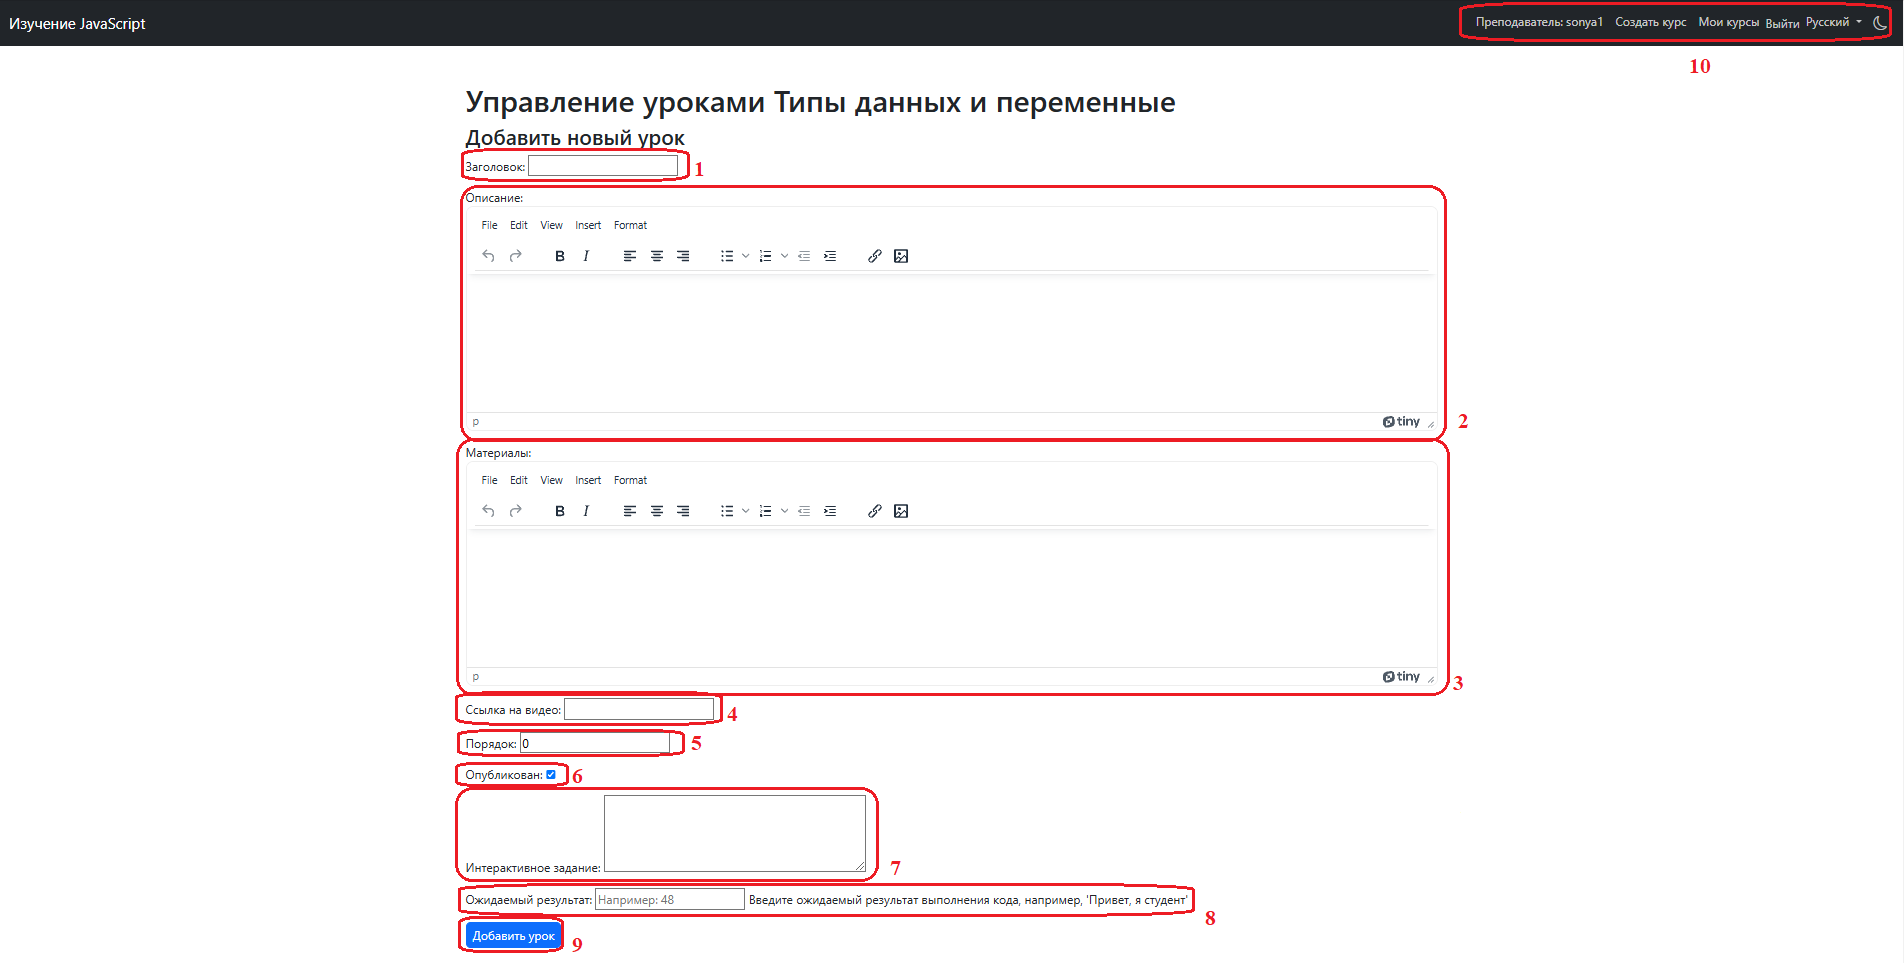
\includegraphics[width=0.9\linewidth]{images/создатьурок}
	\caption{Композиция интерфейса сервиса <<Создание урока>>}
	\label{templ:image10}
\end{figure}

\clearpage
\subsection{Моделирование вариантов использования}

Для разработки платформы была построена UML-диаграмма вариантов использования, отражающая взаимодействие пользователей с системой.

\begin{figure}[ht]
	\center{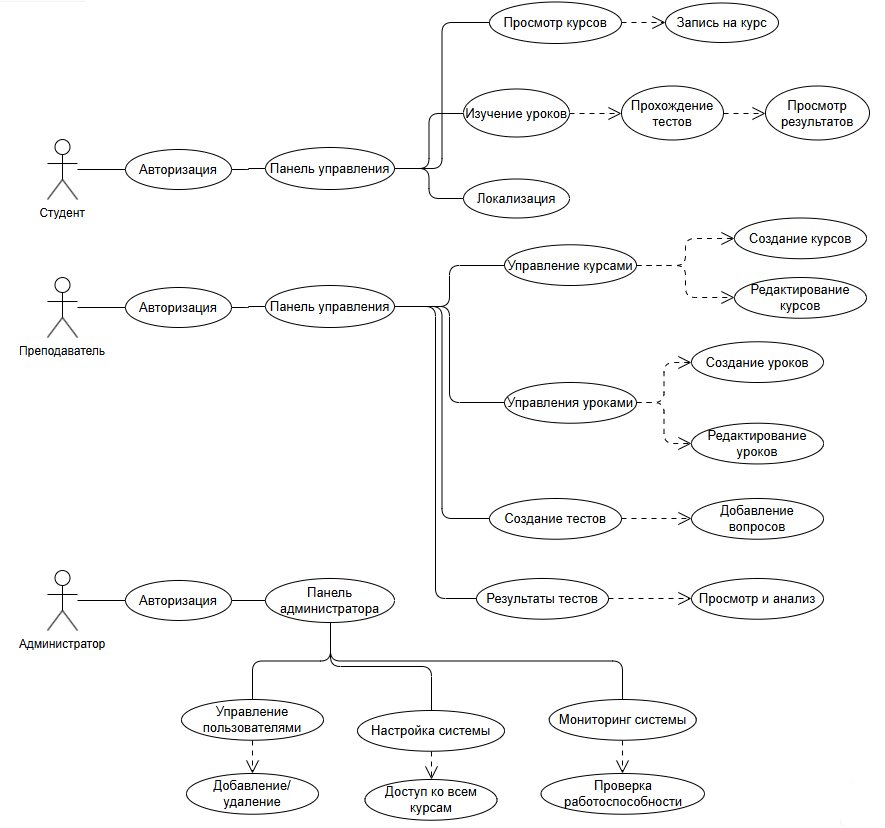
\includegraphics[width=1\linewidth]{images/UML}}
	\caption{Диаграмма прецедентов}
	\label{comp:image}
\end{figure}

Основные прецеденты системы:

\begin{enumerate}
	\item {Авторизация и выход из системы}: Позволяет пользователям (преподавателям, студентам, администраторам) входить в систему и выходить из неё.
	\item {Управление курсами}: Обеспечивает создание, редактирование и удаление курсов преподавателями, а также просмотр и запись на курсы студентами.
	\item {Управление уроками}: Дает возможность преподавателям управлять уроками, а студентам --- изучать их материалы.
	\item {Создание и управление тестами}: Позволяет преподавателям создавать тесты, а студентам --- проходить их.
	\item {Прохождение тестов}: Обеспечивает студентам возможность проходить тесты с автоматической оценкой.
	\item {Просмотр результатов тестов}: Позволяет преподавателям и студентам анализировать результаты.
	\item {Локализация интерфейса}: Обеспечивает переключение языка интерфейса для удобства пользователей.
\end{enumerate}

После авторизации пользователь переходит на главную страницу: преподаватели видят панель управления, студенты --- список доступных курсов. Ниже приведено подробное описание каждого сервиса и связанных прецедентов.

\begin{enumerate}
	\item {Сервис <<Курсы>>}.
	
	{Прецедент: Управление курсами (для преподавателей)}. \\
	{Цель}: Создание, редактирование и удаление курсов. \\
	{Актёр}: Преподаватель. \\
	{Предусловие}: Преподаватель авторизован и находится в панели управления. \\
	{Основной сценарий}:
	\begin{itemize}
		\item преподаватель переходит в раздел <<Курсы>>;
		\item нажимает кнопку <<Создать курс>>;
		\item заполняет форму: название (title), описание (description), изображение (image), статус активности (isactive);
		\item сохраняет курс, система добавляет его в базу данных (courses\_course) и связывает с преподавателем (teacherid);
		\item для редактирования или удаления преподаватель выбирает курс из списка и выполняет соответствующее действие.
	\end{itemize}
	{Постусловие}: Курс создан, отредактирован или удалён, изменения отражены в базе данных. \\
	{Альтернативный сценарий}: Если форма заполнена некорректно (например, пустое название), система выдаёт уведомление об ошибке.
	
	{Прецедент: Просмотр и запись на курсы (для студентов)}. \\
	{Цель}: Просмотр доступных курсов и запись на них. \\
	{Актёр}: Студент. \\
	{Предусловие}: Студент авторизован. \\
	{Основной сценарий}:
	\begin{itemize}
		\item студент переходит на главную страницу, где отображается список курсов;
		\item список включает название, описание и статус курса (например, <<Доступен>>, <<Завершён>>);
		\item студент выбирает курс и нажимает кнопку <<Записаться>>;
		\item система добавляет запись в таблицу <<Запись на курсы>> (courses\_enrollment) с полями (courseid), (studentid), (enrolledat).
	\end{itemize}
	{Постусловие}: Студент записан на курс, запись отражена в базе данных.
	
	\item {Сервис <<Уроки>>}.
	
	{Прецедент: Управление уроками (для преподавателей)}. \\
	{Цель}: Добавление, редактирование, сортировка и удаление уроков в рамках курса. \\
	{Актёр}: Преподаватель. \\
	{Предусловие}: Преподаватель авторизован, выбран курс. \\
	{Основной сценарий}:
	\begin{itemize}
		\item преподаватель переходит в раздел <<Уроки>> выбранного курса;
		\item нажимает кнопку <<Добавить урок>>;
		\item заполняет форму: название (title), описание (description), содержимое (content), ссылка на видео (videourl), порядок (order), статус публикации (ispublished);
		\item сохраняет урок, система добавляет его в таблицу (courses\_lesson);
		\item для сортировки использует интерфейс с Sortable.js, изменяя поле (order);
		\item для редактирования или удаления выбирает урок из списка;
		\item может включить предпросмотр урока перед публикацией.
	\end{itemize}
	{Постусловие}: Урок добавлен, отредактирован, отсортирован или удалён. \\
	{Альтернативный сценарий}: Если видео-URL недействителен, система уведомляет об ошибке.
	
	{Прецедент: Изучение уроков (для студентов)}. \\
	{Цель}: Просмотр материалов урока. \\
	{Актёр}: Студент. \\
	{Предусловие}: Студент записан на курс, урок опубликован. \\
	{Основной сценарий}:
	\begin{itemize}
		\item студент выбирает курс и переходит в раздел <<Уроки>>;
		\item видит список уроков, отсортированных по полю (order);
		\item выбирает урок и просматривает материалы: текст (content), видео (videourl);
		\item после завершения урока система обновляет прогресс (courses\_progress): (completed).
	\end{itemize}
	{Постусловие}: Урок изучен, прогресс обновлён.
	
	\item {Сервис <<Тесты>>}.
	
	{Прецедент: Создание и управление тестами (для преподавателей)}. \\
	{Цель}: Создание тестов с вопросами и ответами. \\
	{Актёр}: Преподаватель. \\
	{Предусловие}: Преподаватель авторизован, выбран урок. \\
	{Основной сценарий}:
	\begin{itemize}
		\item преподаватель переходит в раздел <<Тесты>> урока;
		\item нажимает кнопку <<Создать тест>>;
		\item заполняет форму: название (title), описание (description), проходной балл (passingscore), статус (isactive);
		\item добавляет вопросы (courses\_question): текст (text), тип (questiontype), баллы (points);
		\item для каждого вопроса добавляет варианты ответа (courses\_answer): текст (text), правильность (iscorrect), порядок (order);
		\item сохраняет тест, система добавляет его в таблицу (courses\_test).
	\end{itemize}
	{Постусловие}: Тест создан и связан с уроком (lessonid). \\
	{Альтернативный сценарий}: Если проходной балл некорректен, система выдаёт ошибку.
	
	{Прецедент: Прохождение тестов (для студентов)}. \\
	{Цель}: Прохождение теста и получение оценки. \\
	{Актёр}: Студент. \\
	{Предусловие}: Студент записан на курс, тест активен. \\
	{Основной сценарий}:
	\begin{itemize}
		\item студент переходит к уроку и выбирает тест;
		\item система отображает вопросы с вариантами ответов;
		\item студент выбирает ответы и отправляет тест;
		\item система автоматически оценивает ответы, сравнивая с (iscorrect), и сохраняет результат (courses\_testresult: score, answers, attempts).
	\end{itemize}
	{Постусловие}: Тест пройден, результат сохранён.
	
	\item {Сервис <<Результаты тестов>>}.
	
	{Прецедент: Просмотр и анализ результатов (для преподавателей)}. \\
	{Цель}: Анализ успеваемости студентов. \\
	{Актёр}: Преподаватель. \\
	{Предусловие}: Преподаватель авторизован, тест пройден хотя бы одним студентом. \\
	{Основной сценарий}:
	\begin{itemize}
		\item преподаватель переходит в раздел <<Результаты тестов>>;
		\item система отображает список студентов, их баллы (score), количество попыток (attempts) и ответы (answers);
		\item преподаватель может удалить результат, если он некорректен.
	\end{itemize}
	{Постусловие}: Преподаватель получил статистику по тесту. \\
	{Альтернативный сценарий}: Если результатов нет, отображается сообщение <<Нет данных>>.
	
	{Прецедент: Просмотр результатов (для студентов)}. \\
	{Цель}: Просмотр своих баллов и статистики. \\
	{Актёр}: Студент. \\
	{Предусловие}: Студент прошёл тест. \\
	{Основной сценарий}:
	\begin{itemize}
		\item студент переходит в раздел <<Результаты>>;
		\item система отображает баллы (score), количество попыток (attempts) и правильные/неправильные ответы.
	\end{itemize}
	{Постусловие}: Студент увидел свои результаты.
	
	\item {Сервис <<Локализация>>}.
	
	{Прецедент: Локализация интерфейса}. \\
	{Цель}: Переключение языка интерфейса. \\
	{Актёр}: Любой пользователь (преподаватель, студент). \\
	{Предусловие}: Пользователь авторизован. \\
	{Основной сценарий}:
	\begin{itemize}
		\item пользователь выбирает язык (например, русский или английский) в меню настроек;
		\item система использует Django i18n для переключения языка интерфейса;
		\item страница обновляется с новым языком, включая текст интерфейса и вопросы тестов.
	\end{itemize}
	{Постусловие}: Язык интерфейса изменён. \\
	{Альтернативный сценарий}: Если выбранный язык недоступен, система уведомляет об ошибке.
	
	\item {Сервис <<Уведомления>>}.
	
	{Прецедент: Получение уведомлений}. \\
	{Цель}: Информирование о действиях и ошибках. \\
	{Актёр}: Любой пользователь. \\
	{Предусловие}: Пользователь выполнил действие (например, добавил урок). \\
	{Основной сценарий}:
	\begin{itemize}
		\item после действия (например, добавления урока) система генерирует уведомление (<<Урок успешно добавлен>>);
		\item уведомление отображается в интерфейсе (например, в верхней части страницы);
		\item при ошибке (например, некорректный формат данных) отображается сообщение об ошибке.
	\end{itemize}
	{Постусловие}: Пользователь получил уведомление.
	
	\item {Сервис <<Панель управления>>}.
	
	{Прецедент: Доступ к панели управления (для преподавателей)}. \\
	{Цель}: Быстрый доступ к функциям управления. \\
	{Актёр}: Преподаватель. \\
	{Предусловие}: Преподаватель авторизован. \\
	{Основной сценарий}:
	\begin{itemize}
		\item после авторизации преподаватель переходит на главную страницу;
		\item панель управления отображает виджеты: список курсов, уроки, тесты, результаты;
		\item преподаватель переходит к нужному разделу (например, <<Курсы>>).
	\end{itemize}
	{Постусловие}: Преподаватель получил доступ к функциям управления.
	
	{Прецедент: Доступ к списку курсов (для студентов)}. \\
	{Цель}: Просмотр доступных курсов. \\
	{Актёр}: Студент. \\
	{Предусловие}: Студент авторизован. \\
	{Основной сценарий}:
	\begin{itemize}
		\item после авторизации студент переходит на главную страницу;
		\item система отображает список доступных курсов;
		\item студент выбирает курс для изучения.
	\end{itemize}
	{Постусловие}: Студент получил доступ к курсам.
\end{enumerate}

\subsection{Требования к оформлению документации}

Разработка программной документации и программного изделия должна производиться согласно ГОСТ 19.102–77 и ГОСТ 34.601–90. Единая система программной документации.

\section{Технический проект}

\subsection{Общая характеристика организации решения задачи}

Разработанное веб-приложение представляет собой онлайн-платформу для самостоятельного изучения JavaScript иностранными студентами. Платформа реализована с использованием современных веб-технологий: HTML, CSS, JavaScript и Python (Django). Она размещается в сети Интернет (например, на домене (https://swsueducate.ru) и предоставляет единый пользовательский интерфейс для студентов и преподавателей.

Основные задачи платформы:
\begin{itemize}
	\item управление курсами и уроками;
	\item создание и проведение тестов;
	\item анализ результатов обучения;
	\item поддержка локализации для разных языков.
\end{itemize}

Система построена на клиент-серверной архитектуре:
\begin{enumerate}
	\item {Клиентская часть} (Frontend): Реализована с использованием HTML, CSS (Bootstrap для адаптивности) и JavaScript (включая Sortable.js для сортировки уроков). Отвечает за отображение интерфейса и интерактивность.
	\item {Серверная часть} (Backend): Построена на Django, обрабатывает запросы, управляет данными (через SQLite) и генерирует динамические страницы.
	\item {База данных}: SQLite хранит данные о курсах, уроках, тестах, пользователях и их прогрессе.
\end{enumerate}

\subsection{Архитектура системы}

Архитектура платформы следует модели MVC (Model-View-Controller), реализованной через Django, что обеспечивает чёткое разделение ответственности между компонентами системы. Описание архитектуры:

\begin{enumerate}
	\item {Model} (Модель): Определяет структуру данных в виде таблиц SQLite (courses\_course, courses\_lesson, courses\_test, courses\_question, courses\_answer, users\_user и др.). Модели Django обеспечивают взаимодействие с базой данных через ORM, упрощая операции создания, чтения, обновления и удаления данных (CRUD).
	\item {View} (Представление): Обрабатывает HTTP-запросы и формирует ответы. Включает функции и классы Django views, которые возвращают HTML-страницы (через шаблоны Django) или JSON-ответы для динамической загрузки данных.
	\item {Template} (Шаблоны): Реализован через маршрутизацию Django файл (urls.py), направляющую запросы к соответствующим представлениям.
\end{enumerate}

Основные компоненты системы:
\begin{enumerate}
	\item {Frontend}: Интерфейс пользователя, созданный с помощью шаблонов Django (HTML), стилей Bootstrap и JavaScript. Sortable.js используется для реализации сортировки уроков в интерфейсе преподавателя.
	\item {Backend}: Сервер Django, который управляет логикой приложения, включая аутентификацию (contrib.auth), ограничение доступа (@login\_required) и локализацию (i18n).
	\item {Database}: SQLite, содержащая реляционные таблицы для хранения данных. Использование SQLite обусловлено лёгкостью и достаточной производительностью для данного проекта.
	\item {API}: Внутренние API-методы (реализованы через Django views), обеспечивающие взаимодействие между клиентской и серверной частями, например, для загрузки списка уроков или результатов тестов.
\end{enumerate}

Архитектура представлена на диаграмме компонентов (см. рис.~\ref{diag:image}).
\newpage
\begin{figure}[h]
	\centering{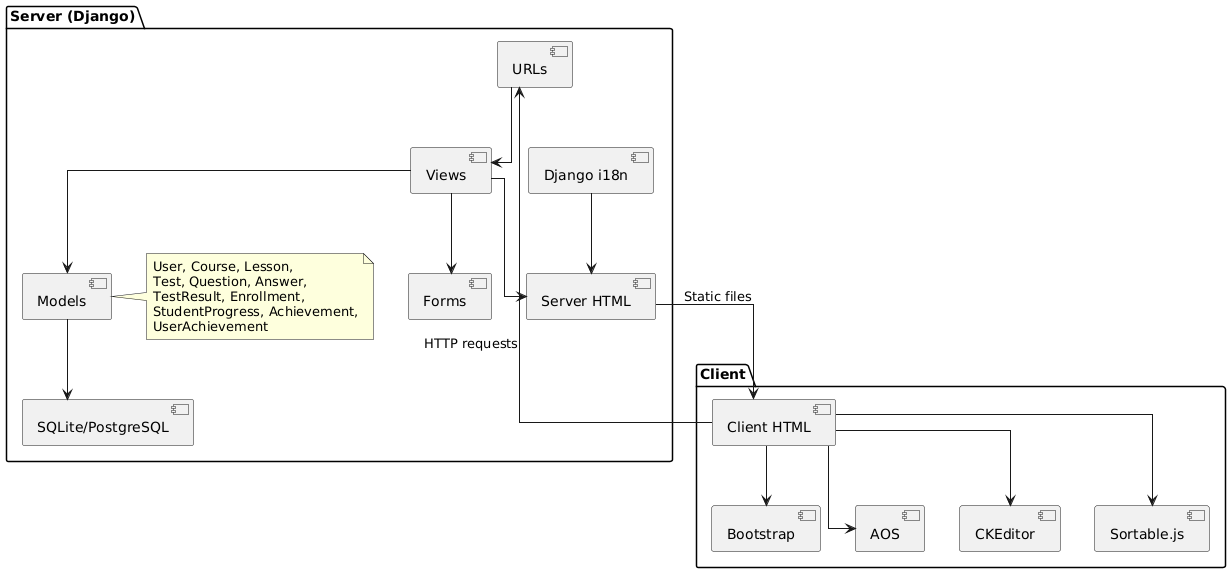
\includegraphics[width=1\linewidth]{images/диаграмма1}}
	\caption{Диаграмма компонентов}
	\label{diag:image}
\end{figure}

\subsection{Структура базы данных}

\subsubsection{Концептуальная модель данных}

На рисунке~\ref{conceptual_model} представлена концептуальная модель данных разрабатываемой обучающей платформы.

\begin{figure}[H]
	\centering
	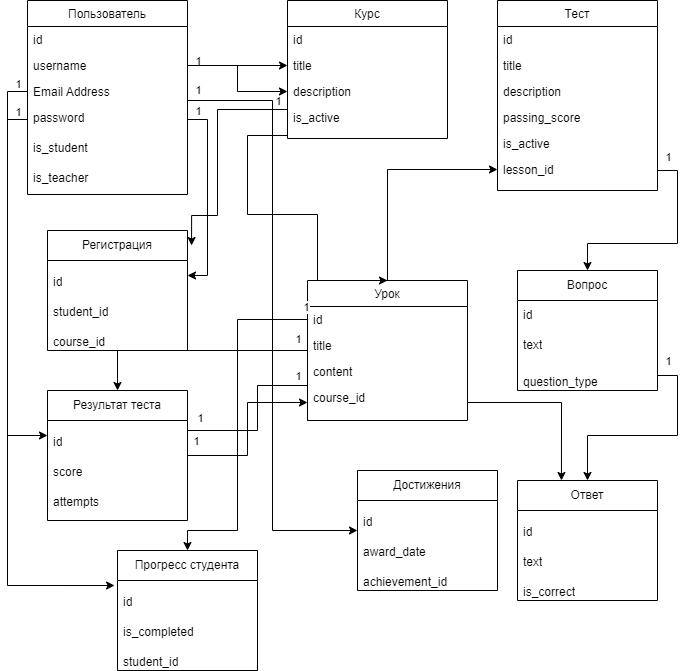
\includegraphics[width=0.95\textwidth]{images/концептуальная}
	\caption{Концептуальная модель данных обучающей платформы}
	\label{conceptual_model}
\end{figure}

Данная модель отражает основные сущности системы и связи между ними на логическом уровне.
Проанализировав требования, выделены следующие основные сущности:
\begin{itemize}
	\item курсы;
	\item уроки;
	\item тесты;
	\item вопросы;
	\item ответы;
	\item результаты тестов;
	\item пользователи;
	\item запись на курсы;
	\item прогресс;
	\item связь пользователей и курсов.
\end{itemize}

\subsubsection{Схема структуры базы данных}

На рисунке~\ref{bd:image} представлена схема структуры базы данных системы, отражающая таблицы, их атрибуты, ключи и связи между ними.

\begin{landscape}
	\begin{figure}[ht]
		\centering
		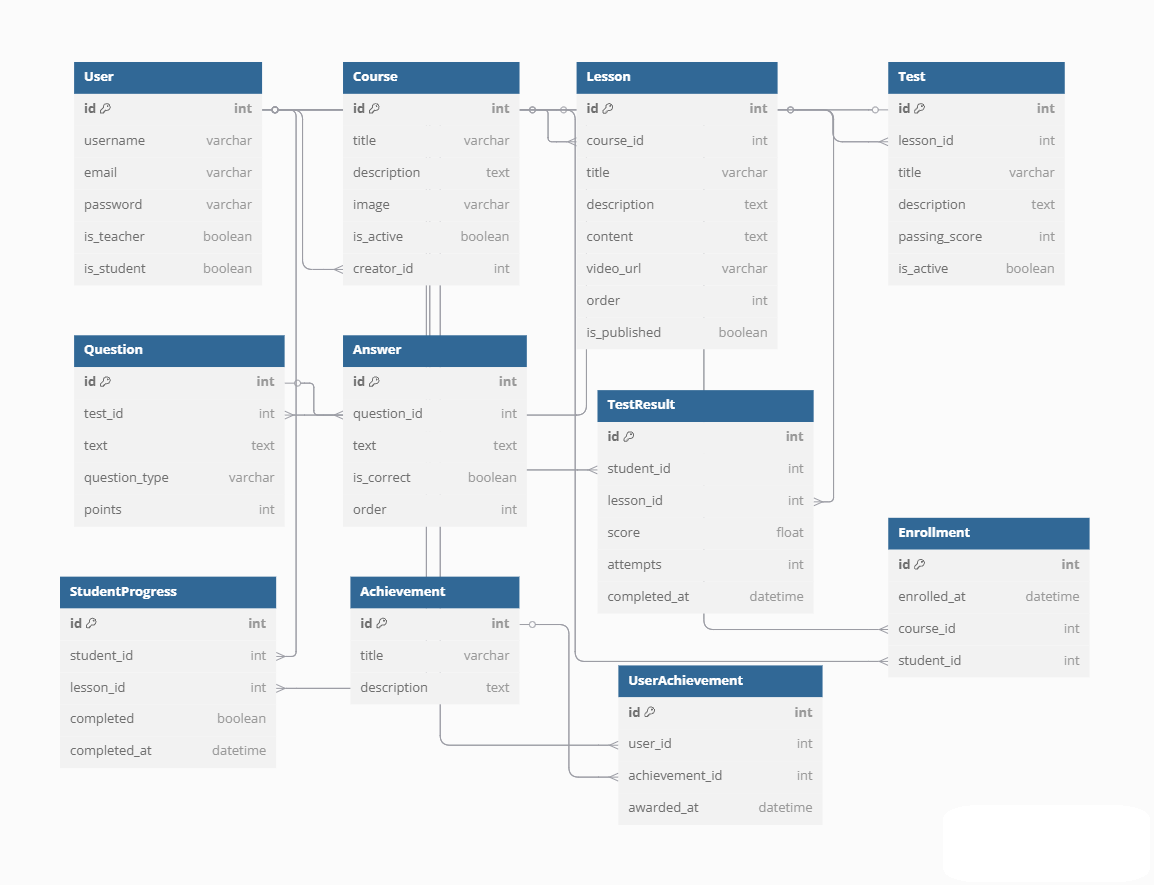
\includegraphics[width=1.3\textwidth]{images/бд} 
		\caption{Структура базы данных}
		\label{bd:image}
	\end{figure}
\end{landscape}

Ниже приведены атрибуты сущностей в формате таблиц.

\begin{xltabular}{\textwidth}{|l|l|p{3.2cm}|X|}
	\caption{Атрибуты сущности <<Курсы>>\label{courses:table}}\\ \hline
	Поле & Тип & Обязательное & Описание \\ \hline
	\endfirsthead
	\continuecaption{Продолжение таблицы \ref{courses:table}}\\ \hline
	Поле & Тип & Обязательное & Описание \\ \hline
	\endhead
	id & Integer & true & Уникальный идентификатор курса \\ \hline
	title & String & true & Название курса \\ \hline
	description & Text & true & Описание курса \\ \hline
	image & String & false & Путь к изображению курса \\ \hline
	isactive & Boolean & true & Признак активности курса \\ \hline
	createdat & DateTime & true & Дата создания курса \\ \hline
	teacherid & ForeignKey & true & Преподаватель (ссылка на таблицу Пользователи) \\ \hline
\end{xltabular}

\begin{xltabular}{\textwidth}{|l|l|p{3.2cm}|X|}
	\caption{Атрибуты сущности <<Уроки>>\label{lessons:table}}\\ \hline
	Поле & Тип & Обязательное & Описание \\ \hline
	\endfirsthead
	\continuecaption{Продолжение таблицы \ref{lessons:table}}\\ \hline
	Поле & Тип & Обязательное & Описание \\ \hline
	\endhead
	id & Integer & true & Уникальный идентификатор урока \\ \hline
	courseid & ForeignKey & true & Курс, к которому относится урок (ссылка на таблицу Курсы) \\ \hline
	title & String & true & Название урока \\ \hline
	description & Text & false & Описание урока \\ \hline
	content & Text & true & Содержимое урока (текст, HTML) \\ \hline
	videourl & String & true & Ссылка на видео урока \\ \hline
	order & Integer & true & Порядок урока в курсе \\ \hline
	ispublished & Boolean & true & Признак публикации урока \\ \hline
	createdat & DateTime & true & Дата создания урока \\ \hline
\end{xltabular}


\begin{xltabular}{\textwidth}{|l|l|p{3.2cm}|X|}
	\caption{Атрибуты сущности <<Тесты>>\label{tests:table}}\\ \hline
	Поле & Тип & Обязательное & Описание \\ \hline
	\endfirsthead
	\continuecaption{Продолжение таблицы \ref{tests:table}}\\ \hline
	Поле & Тип & Обязательное & Описание \\ \hline
	\endhead
	id & Integer & true & Уникальный идентификатор теста \\ \hline
	lessonid & ForeignKey & true & Урок, к которому относится тест (ссылка на таблицу Уроки) \\ \hline
	title & String & true & Название теста \\ \hline
	description & Text & true & Описание теста \\ \hline
	questions & Array & false & Список вопросов (JSON или связанные модели) \\ \hline
	isactive & Boolean & true & Признак активности теста \\ \hline
	passingscore & Integer & true & Проходной балл (в процентах) \\ \hline
	createdat & DateTime & false & Дата создания теста (может отсутствовать) \\ \hline
\end{xltabular}

\begin{xltabular}{\textwidth}{|l|l|p{3.2cm}|X|}
	\caption{Атрибуты сущности <<Результаты тестов>>\label{test_results:table}}\\ \hline
	Поле & Тип & Обязательное & Описание \\ \hline
	\endfirsthead
	\continuecaption{Продолжение таблицы \ref{test_results:table}}\\ \hline
	Поле & Тип & Обязательное & Описание \\ \hline
	\endhead
	id & Integer & true & Уникальный идентификатор результата \\ \hline
	studentid & ForeignKey & true & Студент (ссылка на таблицу Пользователи) \\ \hline
	lessonid & ForeignKey & true & Урок, связанный с тестом (ссылка на таблицу Уроки) \\ \hline
	score & Float & true & Оценка (в процентах или дробное значение) \\ \hline
	attempts & Integer & true & Количество попыток \\ \hline
	answers & Text & true & Ответы (в формате JSON) \\ \hline
	completedat & DateTime & true & Дата завершения теста \\ \hline
\end{xltabular}

\begin{xltabular}{\textwidth}{|l|l|p{3.2cm}|X|}
	\caption{Атрибуты сущности <<Пользователи>>\label{users:table}}\\ \hline
	Поле & Тип & Обязательное & Описание \\ \hline
	\endfirsthead
	\continuecaption{Продолжение таблицы \ref{users:table}}\\ \hline
	Поле & Тип & Обязательное & Описание \\ \hline
	\endhead
	id & Integer & true & Уникальный идентификатор пользователя \\ \hline
	username & String & true & Имя пользователя \\ \hline
	email & String & true & Электронная почта \\ \hline
	isteacher & Boolean & true & Признак преподавателя \\ \hline
	password & String & true & Хэшированный пароль пользователя \\ \hline
	lastlogin & DateTime & false & Дата последнего входа \\ \hline
	issuperuser & Boolean & true & Признак суперпользователя \\ \hline
	firstname & String & true & Имя пользователя \\ \hline
	lastname & String & true & Фамилия пользователя \\ \hline
	isstaff & Boolean & true & Признак персонала \\ \hline
	isactive & Boolean & true & Признак активности пользователя \\ \hline
	datejoined & DateTime & true & Дата регистрации \\ \hline
	isstudent & Boolean & true & Признак студента \\ \hline
	isadmin & Boolean & true & Признак администратора \\ \hline
\end{xltabular}

\begin{xltabular}{\textwidth}{|l|l|p{3.2cm}|X|}
	\caption{Атрибуты сущности <<Запись на курсы>>\label{enrollments:table}}\\ \hline
	Поле & Тип & Обязательное & Описание \\ \hline
	\endfirsthead
	\continuecaption{Продолжение таблицы \ref{enrollments:table}}\\ \hline
	Поле & Тип & Обязательное & Описание \\ \hline
	\endhead
	id & Integer & true & Уникальный идентификатор записи \\ \hline
	enrolledat & DateTime & true & Дата записи на курс \\ \hline
	courseid & ForeignKey & true & Курс (ссылка на таблицу Курсы) \\ \hline
	studentid & ForeignKey & true & Студент (ссылка на таблицу Пользователи) \\ \hline
\end{xltabular}

\begin{xltabular}{\textwidth}{|l|l|p{3.2cm}|X|}
	\caption{Атрибуты сущности <<Прогресс>>\label{progress:table}}\\ \hline
	Поле & Тип & Обязательное & Описание \\ \hline
	\endfirsthead
	\continuecaption{Продолжение таблицы \ref{progress:table}}\\ \hline
	Поле & Тип & Обязательное & Описание \\ \hline
	\endhead
	id & Integer & true & Уникальный идентификатор прогресса \\ \hline
	completed & Boolean & true & Признак завершения урока \\ \hline
	completedat & DateTime & false & Дата завершения урока \\ \hline
	lessonid & ForeignKey & true & Урок (ссылка на таблицу Уроки) \\ \hline
	studentid & ForeignKey & true & Студент (ссылка на таблицу Пользователи) \\ \hline
\end{xltabular}

\begin{xltabular}{\textwidth}{|l|l|p{3.2cm}|X|}
	\caption{Атрибуты сущности <<Вопросы>>\label{questions:table}}\\ \hline
	Поле & Тип & Обязательное & Описание \\ \hline
	\endfirsthead
	\continuecaption{Продолжение таблицы \ref{questions:table}}\\ \hline
	Поле & Тип & Обязательное & Описание \\ \hline
	\endhead
	id & Integer & true & Уникальный идентификатор вопроса \\ \hline
	testid & ForeignKey & true & Тест (ссылка на таблицу Тесты) \\ \hline
	text & Text & true & Текст вопроса \\ \hline
	questiontype & String & true & Тип вопроса (например, выбор, текст) \\ \hline
	points & Integer & true & Баллы за вопрос \\ \hline
\end{xltabular}

\begin{xltabular}{\textwidth}{|l|l|p{3.2cm}|X|}
	\caption{Атрибуты сущности <<Ответы>>\label{answers:table}}\\ \hline
	Поле & Тип & Обязательное & Описание \\ \hline
	\endfirsthead
	\continuecaption{Продолжение таблицы \ref{answers:table} -- Атрибуты сущности <<Ответы>>}\\ \hline
	Поле & Тип & Обязательное & Описание \\ \hline
	\endhead
	id & Integer & true & Уникальный идентификатор ответа \\ \hline
	questionid & ForeignKey & true & Вопрос (ссылка на таблицу Вопросы) \\ \hline
	text & Text & true & Текст ответа \\ \hline
	iscorrect & Boolean & true & Признак правильности ответа \\ \hline
	order & Integer & true & Порядок ответа \\ \hline
\end{xltabular}

\begin{xltabular}{\textwidth}{|l|l|p{3.2cm}|X|}
	\caption{Атрибуты сущности <<Связь пользователей и курсов>>\label{user_courses:table}}\\ \hline
	Поле & Тип & Обязательное & Описание \\ \hline
	\endfirsthead
	\continuecaption{Продолжение таблицы \ref{user_courses:table}}\\ \hline
	Поле & Тип & Обязательное & Описание \\ \hline
	\endhead
	id & Integer & true & Уникальный идентификатор записи \\ \hline
	userid & ForeignKey & true & Пользователь (ссылка на таблицу Пользователи) \\ \hline
	courseid & ForeignKey & true & Курс (ссылка на таблицу Курсы) \\ \hline
\end{xltabular}

Экземпляры этих сущностей реализуются в информационных блоках пользовательского интерфейса. Атрибуты сущностей отображаются в полях, свойствах и компонентах соответствующих элементов.

\subsection{Обоснование выбора технологий}

Для реализации платформы выбраны следующие технологии:
\begin{enumerate}
	\item {Python и Django}: Python обеспечивает простоту и читаемость кода, а Django предоставляет мощный ORM, встроенную аутентификацию (contrib.auth) и локализацию (i18n). Это ускоряет разработку серверной части и упрощает управление данными.
	\item {JavaScript и Sortable.js}: JavaScript отвечает за клиентскую интерактивность (динамическое обновление страниц, обработка событий), а Sortable.js позволяет реализовать сортировку уроков.
	\item {HTML и Bootstrap}: HTML формирует структуру страниц, а Bootstrap обеспечивает адаптивный дизайн, совместимый с различными устройствами.
	\item {SQLite}: Лёгкая реляционная база данных, подходящая для небольшого проекта. SQLite поддерживает все необходимые операции через Django ORM.
\end{enumerate}

Эти технологии выбраны благодаря их совместимости, простоте интеграции и соответствию требованиям проекта. Python и Django обеспечивают надёжную серверную часть, JavaScript и Bootstrap — удобный и отзывчивый интерфейс, а SQLite — эффективное хранение данных.




\ifПрактика{}\else{
   \section{Рабочий проект}

\subsection{Спецификация класса Course}

Модель Course хранит информацию о курсе, созданном преподавателем.

Описание: организует уроки и тесты, поддерживает мультиязычные названия и описания.

Валидация данных:
	\begin{itemize}
		\item поля title, description валидируются через CourseForm;
		\item поле image проверяется на формат (JPEG, PNG).
	\end{itemize}
	
Связи:
	\begin{itemize}
		\item внешний ключ creator на User;
		\item связан с Lesson, Enrollment.
	\end{itemize}
		
Безопасность:
	\begin{itemize}
		\item редактирование доступно только creator через CourseUpdateView;
		\item студенты видят только курсы с isactive=True.
	\end{itemize}
	
Уведомления:
	\begin{itemize}
		\item уведомления через Django messages (например, «Курс создан»).
	\end{itemize}
	
Основные методы:
	\begin{itemize}
		\item str(): возвращает title;
		\item getabsoluteurl(): возвращает URL курса;
		\item save(): обрабатывает изображение.
	\end{itemize}
	
Зависимости:
	\begin{itemize}
		\item связан с Lesson, Test, Enrollment;
		\item использует CKEditor для description.
	\end{itemize}


\begin{xltabular}{\textwidth}{|l|l|l|X|}
	\caption{Данные класса Course\label{tab:course_attributes}}\\
	\hline
	Поле & Тип & Обязательное & Описание \\ \hline
	\endfirsthead
	\continuecaption{Продолжение таблицы \ref{tab:course_attributes}}\\
	\hline
	Поле & Тип & Обязательное & Описание \\ \hline
	\endhead
	id & Integer & да & Уникальный идентификатор \\ \hline
	title & String & да & Название курса \\ \hline
	description & Text & нет & Описание (HTML, CKEditor) \\ \hline
	image & Image & нет & Изображение курса \\ \hline
	isactive & Boolean & да & Статус публикации \\ \hline
	creator & ForeignKey & да & Преподаватель (User) \\ \hline
\end{xltabular}

\begin{xltabular}{\textwidth}{|l|X|}
	\caption{Методы класса Course\label{tab:course_methods}}\\
	\hline
	Метод & Описание \\ \hline
	\endfirsthead
	\continuecaption{Продолжение таблицы \ref{tab:course_methods}}\\
	\hline
	Метод & Описание \\ \hline
	\endhead
	str() & Возвращает title \\ \hline
	getabsoluteurl() & Возвращает URL курса \\ \hline
	save() & Обрабатывает изображение \\ \hline
\end{xltabular}

\begin{lstlisting}[language=Python, caption=Представление для создания курса, label=lst:course_view]
	from django.contrib.auth.decorators import login_required
	from django.shortcuts import render, redirect
	from .models import Course
	from .forms import CourseForm
	
	@login_required
	def create_course(request):
	if not request.user.is_teacher:
	return redirect('home')
	if request.method == 'POST':
	form = CourseForm(request.POST, request.FILES)
	if form.is_valid():
	course = form.save(commit=False)
	course.creator = request.user
	course.save()
	return redirect('courses')
	else:
	form = CourseForm()
	return render(request, 'courses/create.html', {'form': form})
\end{lstlisting}

\subsubsection{Спецификация класса Lesson}

Модель Lesson описывает урок в составе курса.

Описание: хранит контент, видео и упражнения, поддерживает мультиязычность.

Валидация данных:
	\begin{itemize}
		\item поля title, content валидируются через LessonForm;
		\item поле videourl проверяется на корректность.
	\end{itemize}
	
Связи:
	\begin{itemize}
		\item внешний ключ course на Course;
		\item связан с Test, StudentProgress.
	\end{itemize}
	
Безопасность:
	\begin{itemize}
		\item редактирование ограничено creator курса;
		\item доступ для студентов: ispublished=True.
	\end{itemize}
	
Уведомления:
	\begin{itemize}
		\item уведомления через Django messages (например, «Урок добавлен»).
	\end{itemize}
	
Основные методы:
	\begin{itemize}
		\item str(): возвращает title;
		\item save(): проверяет order.
	\end{itemize}
	
Зависимости:
	\begin{itemize}
		\item связан с Course, Test, StudentProgress;
		\item использует CKEditor для content.
	\end{itemize}


\begin{xltabular}{\textwidth}{|l|l|l|X|}
	\caption{Данные класса Lesson\label{tab:lesson_attributes}}\\
	\hline
	Поле & Тип & Обязательное & Описание \\ \hline
	\endfirsthead
	\continuecaption{Продолжение таблицы \ref{tab:lesson_attributes}}\\
	\hline
	Поле & Тип & Обязательное & Описание \\ \hline
	\endhead
	id & Integer & да & Уникальный идентификатор \\ \hline
	title & String & да & Название урока \\ \hline
	content & Text & да & Содержимое (HTML, CKEditor) \\ \hline
	videourl & URL & нет & Ссылка на видео \\ \hline
	order & Integer & да & Порядок урока \\ \hline
	ispublished & Boolean & да & Статус публикации \\ \hline
	exercise & Text & нет & Интерактивное упражнение \\ \hline
	expectedresult & Text & нет & Ожидаемый результат \\ \hline
	course & ForeignKey & да & Курс (Course) \\ \hline
\end{xltabular}

\begin{xltabular}{\textwidth}{|l|X|}
	\caption{Методы класса Lesson\label{tab:lesson_methods}}\\
	\hline
	Метод & Описание \\ \hline
	\endfirsthead
	\continuecaption{Продолжение таблицы \ref{tab:lesson_methods}}\\
	\hline
	Метод & Описание \\ \hline
	\endhead
	str() & Возвращает title \\ \hline
	save() & Проверяет order \\ \hline
\end{xltabular}

\subsubsection{Спецификация класса Test}

Модель Test описывает тест, связанный с уроком.

Описание: проверяет знания студентов, поддерживает мультиязычные вопросы.

Валидация данных:
	\begin{itemize}
		\item поля title, description валидируются через TestForm;
		\item поле passingscore — положительное значение.
	\end{itemize}
	
Связи:
	\begin{itemize}
		\item внешний ключ lesson на Lesson;
		\item связан с Question, TestResult.
	\end{itemize}
	
Безопасность:
	\begin{itemize}
		\item редактирование ограничено creator урока;
		\item доступ для студентов: isactive=True.
	\end{itemize}
	
Уведомления:
	\begin{itemize}
		\item уведомления через Django messages (например, «Тест создан»).
	\end{itemize}
	
Основные методы:
	\begin{itemize}
		\item str(): возвращает title;
		\item save(): проверяет passingscore.
	\end{itemize}
	
Зависимости:
	\begin{itemize}
		\item связан с Lesson, Question, TestResult;
		\item используется в testform.html.
	\end{itemize}


\begin{xltabular}{\textwidth}{|l|l|l|X|}
	\caption{Данные класса Test\label{tab:test_attributes}}\\
	\hline
	Поле & Тип & Обязательное & Описание \\ \hline
	\endfirsthead
	\continuecaption{Продолжение таблицы \ref{tab:test_attributes}}\\
	\hline
	Поле & Тип & Обязательное & Описание \\ \hline
	\endhead
	id & Integer & да & Уникальный идентификатор \\ \hline
	title & String & да & Название теста \\ \hline
	description & Text & нет & Описание теста \\ \hline
	passingscore & Integer & да & Проходной балл \\ \hline
	isactive & Boolean & да & Статус активности \\ \hline
	lesson & ForeignKey & да & Урок (Lesson) \\ \hline
\end{xltabular}

\begin{xltabular}{\textwidth}{|l|X|}
	\caption{Методы класса Test\label{tab:test_methods}}\\
	\hline
	Метод & Описание \\ \hline
	\endfirsthead
	\continuecaption{Продолжение таблицы \ref{tab:test_methods}}\\
	\hline
	Метод & Описание \\ \hline
	\endhead
	str() & Возвращает title \\ \hline
	save() & Проверяет passingscore \\ \hline
\end{xltabular}

\subsubsection{Спецификация класса Question}

Модель Question описывает вопрос в тесте.


Описание: поддерживает различные типы вопросов (одиночный, множественный, текстовый) с мультиязычным текстом.

Валидация данных:
	\begin{itemize}
		\item поле text валидируется через QuestionForm;
		\item поле questiontype принимает значения single, multiple, text;
		\item поле points проверяется на положительное значение.
	\end{itemize}
	
Связи:
	\begin{itemize}
		\item внешний ключ test на Test;
		\item связан с Answer.
	\end{itemize}
	
Безопасность:
	\begin{itemize}
		\item редактирование ограничено creator урока через представления;
		\item доступ для студентов только через активные тесты.
	\end{itemize}
	
Уведомления:
	\begin{itemize}
		\item уведомления через Django messages (например, «Вопрос добавлен»).
	\end{itemize}
	
Основные методы:
	\begin{itemize}
		\item str(): возвращает text;
		\item save(): проверяет questiontype и points.
	\end{itemize}
	
Зависимости:
	\begin{itemize}
		\item связан с Test, Answer;
		\item используется в шаблоне questionform.html.
	\end{itemize}


\begin{xltabular}{\textwidth}{|l|l|l|X|}
	\caption{Данные класса Question\label{tab:question_attributes}}\\
	\hline
	Поле & Тип & Обязательное & Описание \\ \hline
	\endfirsthead
	\continuecaption{Продолжение таблицы \ref{tab:question_attributes}}\\
	\hline
	Поле & Тип & Обязательное & Описание \\ \hline
	\endhead
	id & Integer & да & Уникальный идентификатор \\ \hline
	text & Text & да & Текст вопроса \\ \hline
	questiontype & String & да & Тип вопроса (single, multiple, text) \\ \hline
	points & Integer & да & Баллы за ответ \\ \hline
	test & ForeignKey & да & Тест (Test) \\ \hline
\end{xltabular}

\begin{xltabular}{\textwidth}{|l|X|}
	\caption{Методы класса Question\label{tab:question_methods}}\\
	\hline
	Метод & Описание \\ \hline
	\endfirsthead
	\continuecaption{Продолжение таблицы \ref{tab:question_methods}}\\
	\hline
	Метод & Описание \\ \hline
	\endhead
	str() & Возвращает text \\ \hline
	save() & Проверяет questiontype и points \\ \hline
\end{xltabular}

\subsubsection{Спецификация класса Answer}

Модель Answer описывает вариант ответа на вопрос в тесте.

Описание: хранит текст ответа и флаг правильности, поддерживает мультиязычность.

Валидация данных:
	\begin{itemize}
		\item поле text валидируется через AnswerForm;
		\item поле iscorrect — булево, проверяется на уровне формы;
		\item поле order проверяется на положительное значение.
	\end{itemize}
	
Связи:
	\begin{itemize}
		\item внешний ключ question на Question;
		\item используется в TestResult.
	\end{itemize}
	
Безопасность:
	\begin{itemize}
		\item редактирование ограничено creator урока через AnswerCreateView;
		\item доступ для студентов только через активные тесты.
	\end{itemize}
	
Уведомления:
	\begin{itemize}
		\item уведомления через Django messages (например, «Ответ добавлен»).
	\end{itemize}
	
Лсновные методы:
	\begin{itemize}
		\item str(): возвращает text;
		\item save(): проверяет iscorrect и order.
	\end{itemize}
	
Зависимости:
	\begin{itemize}
		\item связан с Question, TestResult;
		\item используется в шаблоне answerform.html.
	\end{itemize}


\begin{xltabular}{\textwidth}{|l|l|l|X|}
	\caption{Данные класса Answer\label{tab:answer_attributes}}\\
	\hline
	Поле & Тип & Обязательное & Описание \\ \hline
	\endfirsthead
	\continuecaption{Продолжение таблицы \ref{tab:answer_attributes}}\\
	\hline
	Поле & Тип & Обязательное & Описание \\ \hline
	\endhead
	id & Integer & да & Уникальный идентификатор \\ \hline
	text & Text & да & Текст ответа \\ \hline
	iscorrect & Boolean & да & Признак правильности \\ \hline
	order & Integer & да & Порядок отображения \\ \hline
	question & ForeignKey & да & Вопрос (Question) \\ \hline
\end{xltabular}

\begin{xltabular}{\textwidth}{|l|X|}
	\caption{Методы класса Answer\label{tab:answer_methods}}\\
	\hline
	Метод & Описание \\ \hline
	\endfirsthead
	\continuecaption{Продолжение таблицы \ref{tab:answer_methods}}\\
	\hline
	Метод & Описание \\ \hline
	\endhead
	str() & Возвращает text \\ \hline
	save() & Проверяет iscorrect и order \\ \hline
\end{xltabular}

\subsubsection{Спецификация класса TestResult}

Модель TestResult хранит результаты прохождения тестов студентами.


Описание: фиксирует баллы, выбранные ответы и дату завершения.

Валидация данных:
	\begin{itemize}
		\item поле score проверяется на положительное значение и соответствие максимуму теста;
		\item поле answers валидируется через TestSubmissionForm.
	\end{itemize}
	
Связи:
	\begin{itemize}
		\item внешний ключ student на User;
		\item внешний ключ lesson на Lesson;
		\item связь ManyToMany с Answer.
	\end{itemize}
	
Безопасность:
	\begin{itemize}
		\item доступ ограничен student или creator урока через представления;
		\item результаты видны только авторизованным пользователям.
	\end{itemize}
	
Уведомления:
	\begin{itemize}
		\item уведомления через Django messages (например, «Тест успешно пройден»).
	\end{itemize}
	
Основные методы:
	\begin{itemize}
		\item str(): возвращает информацию о результате (например, «Результат студента X по уроку Y»);
		\item save(): пересчитывает score на основе answers.
	\end{itemize}
	
Зависимости:
	\begin{itemize}
		\item связан с User, Lesson, Answer;
		\item используется в шаблоне testresult.html.
	\end{itemize}


\begin{xltabular}{\textwidth}{|l|l|l|X|}
	\caption{Данные класса TestResult\label{tab:testresult_attributes}}\\
	\hline
	Поле & Тип & Обязательное & Описание \\ \hline
	\endfirsthead
	\continuecaption{Продолжение таблицы \ref{tab:testresult_attributes}}\\
	\hline
	Поле & Тип & Обязательное & Описание \\ \hline
	\endhead
	id & Integer & да & Уникальный идентификатор \\ \hline
	student & ForeignKey & да & Студент (User) \\ \hline
	lesson & ForeignKey & да & Урок (Lesson) \\ \hline
	score & Integer & да & Полученные баллы \\ \hline
	answers & ManyToMany & да & Выбранные ответы \\ \hline
	attempts & Integer & да & Количество попыток \\ \hline
	completedat & DateTime & да & Дата завершения \\ \hline
\end{xltabular}

\begin{xltabular}{\textwidth}{|l|X|}
	\caption{Методы класса TestResult\label{tab:testresult_methods}}\\
	\hline
	Метод & Описание \\ \hline
	\endfirsthead
	\continuecaption{Продолжение таблицы \ref{tab:testresult_methods}}\\
	\hline
	Метод & Описание \\ \hline
	\endhead
	str() & Возвращает информацию о результате \\ \hline
	save() & Пересчитывает score \\ \hline
\end{xltabular}

\subsubsection{Спецификация класса Enrollment}

Модель Enrollment фиксирует запись студента на курс.


Описание: связывает студента и курс для отслеживания участия.

Валидация данных:
	\begin{itemize}
		\item поля student и course проверяются на уникальность через uniquetogether.
	\end{itemize}
	
Связи:
	\begin{itemize}
		\item внешний ключ student на User;
		\item внешний ключ course на Course.
	\end{itemize}
	
Безопасность:
	\begin{itemize}
		\item доступ ограничен student или преподавателю через представления;
		\item преподаватели видят записи через teacherdashboard.
	\end{itemize}
	
Уведомления:
	\begin{itemize}
		\item уведомления через Django messages (например, «Вы записаны на курс»).
	\end{itemize}
	
Основные методы:
	\begin{itemize}
		\item str(): возвращает информацию о записи (например, «Студент X записан на курс Y»);
		\item save(): проверяет уникальность записи.
	\end{itemize}
	
Зависимости:
	\begin{itemize}
		\item связан с User, Course;
		\item используется в представлениях enrollcourse, unenrollcourse.
	\end{itemize}


\begin{xltabular}{\textwidth}{|l|l|l|X|}
	\caption{Данные класса Enrollment\label{tab:enrollment_attributes}}\\
	\hline
	Поле & Тип & Обязательное & Описание \\ \hline
	\endfirsthead
	\continuecaption{Продолжение таблицы \ref{tab:enrollment_attributes}}\\
	\hline
	Поле & Тип & Обязательное & Описание \\ \hline
	\endhead
	id & Integer & да & Уникальный идентификатор \\ \hline
	student & ForeignKey & да & Студент (User) \\ \hline
	course & ForeignKey & да & Курс (Course) \\ \hline
\end{xltabular}

\begin{xltabular}{\textwidth}{|l|X|}
	\caption{Методы класса Enrollment\label{tab:enrollment_methods}}\\
	\hline
	Метод & Описание \\ \hline
	\endfirsthead
	\continuecaption{Продолжение таблицы \ref{tab:enrollment_methods}}\\
	\hline
	Метод & Описание \\ \hline
	\endhead
	str() & Возвращает информацию о записи \\ \hline
	save() & Проверяет уникальность \\ \hline
\end{xltabular}

\subsubsection{Спецификация класса StudentProgress}

Модель StudentProgress отслеживает прогресс студента по урокам.


Описание: фиксирует завершённость уроков и дату завершения.

Валидация данных:
	\begin{itemize}
		\item поле completed — булево, устанавливается через представления;
		\item поле completedat заполняется автоматически при completed=True.
	\end{itemize}
	
Связи:
	\begin{itemize}
		\item внешний ключ student на User;
		\item внешний ключ lesson на Lesson.
	\end{itemize}
	
Безопасность:
	\begin{itemize}
		\item доступ ограничен student через представления;
		\item преподаватели видят прогресс через teacherdashboard.
	\end{itemize}
	
Уведомления:
	\begin{itemize}
		\item уведомления через Django messages (например, «Урок завершён»).
	\end{itemize}
	
Основные методы:
	\begin{itemize}
		\item str(): возвращает информацию о прогрессе (например, «Прогресс студента X по уроку Y»);
		\item save(): устанавливает completedat.
	\end{itemize}
	
Зависимости:
	\begin{itemize}
		\item связан с User, Lesson;
		\item используется в представлениях completelesson, studentdashboard.
	\end{itemize}


\begin{xltabular}{\textwidth}{|l|l|l|X|}
	\caption{Данные класса StudentProgress\label{tab:studentprogress_attributes}}\\
	\hline
	Поле & Тип & Обязательное & Описание \\ \hline
	\endfirsthead
	\continuecaption{Продолжение таблицы \ref{tab:studentprogress_attributes}}\\
	\hline
	Поле & Тип & Обязательное & Описание \\ \hline
	\endhead
	id & Integer & да & Уникальный идентификатор \\ \hline
	student & ForeignKey & да & Студент (User) \\ \hline
	lesson & ForeignKey & да & Урок (Lesson) \\ \hline
	completed & Boolean & да & Завершённость урока \\ \hline
	completedat & DateTime & нет & Дата завершения \\ \hline
\end{xltabular}

\begin{xltabular}{\textwidth}{|l|X|}
	\caption{Методы класса StudentProgress\label{tab:studentprogress_methods}}\\
	\hline
	Метод & Описание \\ \hline
	\endfirsthead
	\continuecaption{Продолжение таблицы \ref{tab:studentprogress_methods}}\\
	\hline
	Метод & Описание \\ \hline
	\endhead
	str() & Возвращает информацию о прогрессе \\ \hline
	save() & Устанавливает completedat \\ \hline
\end{xltabular}

\subsubsection{Спецификация класса Achievement}

Модель Achievement описывает достижения, присваиваемые студентам.


Описание: хранит информацию о наградах (например, «Первый завершённый урок»)).

Валидация данных:
	\begin{itemize}
		\item поля title, description валидируются через AchievementForm;
		\item проверка уникальности title через Django ORM.
	\end{itemize}
	
Связи:
	\begin{itemize}
		\item связан с UserAchievement через внешний ключ.
	\end{itemize}
	
Безопасность:
	\begin{itemize}
		\item редактирование ограничено администраторам через isstaff.
	\end{itemize}
	
Уведомления:
	\begin{itemize}
		\item уведомления через Django messages (например, «Достижение создано»).
	\end{itemize}
	
Основные методы:
	\begin{itemize}
		\item str(): возвращает title;
		\item save(): проверяет уникальность title.
	\end{itemize}
	
Зависимости:
	\begin{itemize}
		\item связан с UserAchievement;
		\item используется в studentdashboard.
	\end{itemize}


\begin{xltabular}{\textwidth}{|l|l|l|X|}
	\caption{Данные класса Achievement\label{tab:achievement_attributes}}\\
	\hline
	Поле & Тип & Обязательное & Описание \\ \hline
	\endfirsthead
	\continuecaption{Продолжение таблицы \ref{tab:achievement_attributes}}\\
	\hline
	Поле & Тип & Обязательное & Описание \\ \hline
	\endhead
	id & Integer & да & Уникальный идентификатор \\ \hline
	title & String & да & Название достижения \\ \hline
	description & Text & нет & Описание достижения \\ \hline
\end{xltabular}

\begin{xltabular}{\textwidth}{|l|X|}
	\caption{Методы класса Achievement\label{tab:achievement_methods}}\\
	\hline
	Метод & Описание \\ \hline
	\endfirsthead
	\continuecaption{Продолжение таблицы \ref{tab:achievement_methods}}\\
	\hline
	Метод & Описание \\ \hline
	\endhead
	str() & Возвращает title \\ \hline
	save() & Проверяет уникальность title \\ \hline
\end{xltabular}

\subsubsection{Спецификация класса UserAchievement}

Модель UserAchievement связывает пользователей с достижениями.


Описание: отслеживает, какие достижения присвоены студентам.

Валидация данных:
	\begin{itemize}
		\item поля user и achievement проверяются на уникальность через uniquetogether.
	\end{itemize}
	
Связи:
	\begin{itemize}
		\item внешний ключ user на User;
		\item внешний ключ achievement на Achievement.
	\end{itemize}
	
Безопасность:
	\begin{itemize}
		\item доступ ограничен user через представления;
		\item преподаватели видят достижения через teacherdashboard.
	\end{itemize}
	
Уведомления:
	\begin{itemize}
		\item уведомления через Django messages (например, «Новое достижение получено»).
	\end{itemize}
	
Основные методы:
	\begin{itemize}
		\item str(): возвращает информацию о достижении (например, «Достижение X для пользователя Y»);
		\item save(): проверяет уникальность связи.
	\end{itemize}
	
Зависимости:
	\begin{itemize}
		\item связан с User, Achievement;
		\item используется в studentdashboard.
	\end{itemize}


\begin{xltabular}{\textwidth}{|l|l|l|X|}
	\caption{Данные класса UserAchievement\label{tab:userachievement_attributes}}\\
	\hline
	Поле & Тип & Обязательное & Описание \\ \hline
	\endfirsthead
	\continuecaption{Продолжение таблицы \ref{tab:userachievement_attributes}}\\
	\hline
	Поле & Тип & Обязательное & Описание \\ \hline
	\endhead
	id & Integer & да & Уникальный идентификатор \\ \hline
	user & ForeignKey & да & Пользователь (User) \\ \hline
	achievement & ForeignKey & да & Достижение (Achievement) \\ \hline
	awardedat & DateTime & да & Дата присвоения \\ \hline
\end{xltabular}

\begin{xltabular}{\textwidth}{|l|X|}
	\caption{Методы класса UserAchievement\label{tab:userachievement_methods}}\\
	\hline
	Метод & Описание \\ \hline
	\endfirsthead
	\continuecaption{Продолжение таблицы \ref{tab:userachievement_methods}}\\
	\hline
	Метод & Описание \\ \hline
	\endhead
	str() & Возвращает информацию о достижении \\ \hline
	save() & Проверяет уникальность связи \\ \hline
\end{xltabular}

\subsection{Модульное тестирование классов и методов программы}

Модульное тестирование проводилось для проверки корректности работы всех классов и методов обучающей платформы, разработанной на Django. Тестирование выполнялось с использованием фреймворка django.test, который позволяет создавать изолированные тестовые сценарии для моделей, представлений и форм.

Тестируемые компоненты:
\begin{enumerate}
	\item Модель User: проверка создания пользователей с ролями студента и преподавателя.
	\begin{lstlisting}[language=Python, caption=Модульный тест для User, label=lst:user_test]
		from django.test import TestCase
		from django.contrib.auth import get_user_model
		
		User = get_user_model()
		
		class UserTestCases(TestCase):
		def setUp(self):
		self.teacher = User.objects.create_user(
		username='sonya1',
		password='vanya232323',
		is_teacher=True
		)
		self.student = User.objects.create_user(
		username='Ivan_Sedih',
		password='vanya232323',
		is_student=True
		)
		
		def test_user_creation(self):
		self.assertTrue(self.teacher.is_teacher)
		self.assertTrue(self.student.is_student)
	\end{lstlisting}
	
	\item Модель Course: проверка создания курса, валидации полей и связи с создателем.
	\begin{lstlisting}[language=Python, caption=Модульный тест для Course, label=lst:course_test]
		from django.test import TestCase
		from learning.models import Course
		from django.contrib.auth import get_user_model
		
		User = get_user_model()
		
		class CourseTestCases(TestCase):
		def setUp(self):
		self.teacher = User.objects.create_user(username='sonya1', password='vanya232323', is_teacher=True)
		self.course = Course.objects.create(
		title='Основы JS',
		description='Описание курса',
		creator=self.teacher,
		is_active=True
		)
		
		def test_course_creation(self):
		self.assertEqual(self.course.title, 'Основы JS')
		self.assertEqual(self.course.creator, self.teacher)
		self.assertTrue(self.course.is_active)
	\end{lstlisting}
	
	\item Модель Lesson: проверка добавления урока, порядка и связи с курсом.
	\begin{lstlisting}[language=Python, caption=Модульный тест для Lesson, label=lst:lesson_test]
		from django.test import TestCase
		from learning.models import Course, Lesson
		from django.contrib.auth import get_user_model
		
		User = get_user_model()
		
		class LessonTestCases(TestCase):
		def setUp(self):
		self.teacher = User.objects.create_user(username='sonya1', password='vanya232323', is_teacher=True)
		self.course = Course.objects.create(title='Массивы', description='Описание курса', creator=self.teacher)
		self.lesson = Lesson.objects.create(
		title='Что такое массивы',
		content='Содержимое урока',
		order=1,
		course=self.course,
		is_published=True
		)
		
		def test_lesson_creation(self):
		self.assertEqual(self.lesson.title, 'Что такое массивы')
		self.assertEqual(self.lesson.order, 1)
		self.assertEqual(self.lesson.course, self.course)
	\end{lstlisting}
	
	\item Модель Test: проверка создания тестов и связи с уроком.
	\begin{lstlisting}[language=Python, caption=Модульный тест для Test, label=lst:test_test]
		from django.test import TestCase
		from learning.models import Test, Lesson, Course
		from django.contrib.auth import get_user_model
		
		User = get_user_model()
		
		class TestTestCases(TestCase):
		def setUp(self):
		self.teacher = User.objects.create_user(username='sonya1', password='vanya232323', is_teacher=True)
		self.course = Course.objects.create(title='Массивы', description='Описание курса', creator=self.teacher)
		self.lesson = Lesson.objects.create(title='Поиск индекса элемента в массиве', content='Содержимое урока', order=1, course=self.course)
		self.test = Test.objects.create(
		title='Тест',
		passing_score=80,
		lesson=self.lesson,
		is_active=True
		)
		
		def test_test_creation(self):
		self.assertEqual(self.test.title, 'Тест')
		self.assertEqual(self.test.passing_score, 80)
		self.assertEqual(self.test.lesson, self.lesson)
	\end{lstlisting}
	
	\item Модель TestResult: проверка сохранения результатов тестов.
	\begin{lstlisting}[language=Python, caption=Модульный тест для TestResult, label=lst:testresult_test]
		from django.test import TestCase
		from learning.models import TestResult, Test, Lesson, Course
		from django.contrib.auth import get_user_model
		from django.utils import timezone
		
		User = get_user_model()
		
		class TestResultTestCases(TestCase):
		def setUp(self):
		self.teacher = User.objects.create_user(username='sonya1', password='vanya232323', is_teacher=True)
		self.student = User.objects.create_user(username='Ivan_Sedih', password='vanya232323', is_student=True)
		self.course = Course.objects.create(title='Объекты', description='Описание курса', creator=self.teacher)
		self.lesson = Lesson.objects.create(title='Создание объектов', content='Содержимое урока', order=1, course=self.course)
		self.test = Test.objects.create(title='Тест', passing_score=70, lesson=self.lesson)
		self.test_result = TestResult.objects.create(
		student=self.student,
		lesson=self.lesson,
		score=85,
		answers='{"q1": "a1"}',
		attempts=1,
		completed_at=timezone.now()
		)
		
		def test_testresult_creation(self):
		self.assertEqual(self.test_result.score, 85)
		self.assertEqual(self.test_result.student, self.student)
		self.assertEqual(self.test_result.lesson, self.lesson)
	\end{lstlisting}
	
	\item Модель StudentProgress: проверка отметки о завершении урока.
	\begin{lstlisting}[language=Python, caption=Модульный тест для StudentProgress, label=lst:studentprogress_test]
		from django.test import TestCase
		from learning.models import StudentProgress, Lesson, Course
		from django.contrib.auth import get_user_model
		from django.utils import timezone
		
		User = get_user_model()
		
		class StudentProgressTestCases(TestCase):
		def setUp(self):
		self.teacher = User.objects.create_user(username='sonya1', password='vanya232323', is_teacher=True)
		self.student = User.objects.create_user(username='Ivan_Sedih', password='vanya232323', is_student=True)
		self.course = Course.objects.create(title='Типы данных', description='Описание курса', creator=self.teacher)
		self.lesson = Lesson.objects.create(title='Переменные', content='Содержимое урока', order=1, course=self.course)
		self.progress = StudentProgress.objects.create(
		student=self.student,
		lesson=self.lesson,
		completed=True,
		completed_at=timezone.now()
		)
		
		def test_studentprogress_creation(self):
		self.assertTrue(self.progress.completed)
		self.assertEqual(self.progress.student, self.student)
		self.assertEqual(self.progress.lesson, self.lesson)
	\end{lstlisting}
	
	\item Модель UserAchievement: проверка присвоения достижений пользователям.
	\begin{lstlisting}[language=Python, caption=Модульный тест для UserAchievement, label=lst:userachievement_test]
		from django.test import TestCase
		from learning.models import Achievement, UserAchievement
		from django.contrib.auth import get_user_model
		from django.utils import timezone
		
		User = get_user_model()
		
		class UserAchievementTestCases(TestCase):
		def setUp(self):
		self.student = User.objects.create_user(username='Ivan_Sedih', password='vanya232323', is_student=True)
		self.achievement = Achievement.objects.create(
		title='Завершение теста',
		description='Сдан первый тест',
		badge_image='badges/test_completed.png'
		)
		self.user_achievement = UserAchievement.objects.create(
		user=self.student,
		achievement=self.achievement,
		awarded_at=timezone.now()
		)
		
		def test_userachievement_creation(self):
		self.assertEqual(self.user_achievement.user, self.student)
		self.assertEqual(self.user_achievement.achievement, self.achievement)
	\end{lstlisting}
\end{enumerate}

Инструменты: django.test.TestCase, unittest.\\
Результаты: все тесты выполнены успешно, ошибок не обнаружено.


\subsection{Системное тестирование разработанного веб-приложения}

Системное тестирование проводилось для проверки взаимодействия компонентов и интерфейса.

Сценарии тестирования:
	\begin{enumerate}
	\item Регистрация и авторизация пользователя.
	\item Создание курса и запись студента.
	\item Добавление урока с контентом через CKEditor.
	\item Прохождение теста и просмотр результатов.
	\item Присвоение достижения студенту.
	\item Редактирование курса.
	\item Удаление курса.
	\item Переупорядочивание уроков.
	\item Проверка доступа к уроку.
	\item Просмотр прогресса студента.
	\item Управление вопросами и ответами теста.
	\end{enumerate}


Описание сценариев тестирования:


	
\subsubsection{Регистрация и авторизация пользователя}
	
Описание: пользователь должен иметь возможность зарегистрироваться в системе, выбрав роль (преподаватель или студент), и войти с использованием учетных данных (имя пользователя, пароль, email).
	
Ожидаемый результат: при успешной регистрации и вводе верных учетных данных осуществляется вход, открывается главная рабочая область (панель управления для преподавателя или каталог курсов для студента). При вводе некорректных данных система отображает сообщение об ошибке (например, "Пользователь не найден").
	
	\begin{figure}[ht]
		\centering
		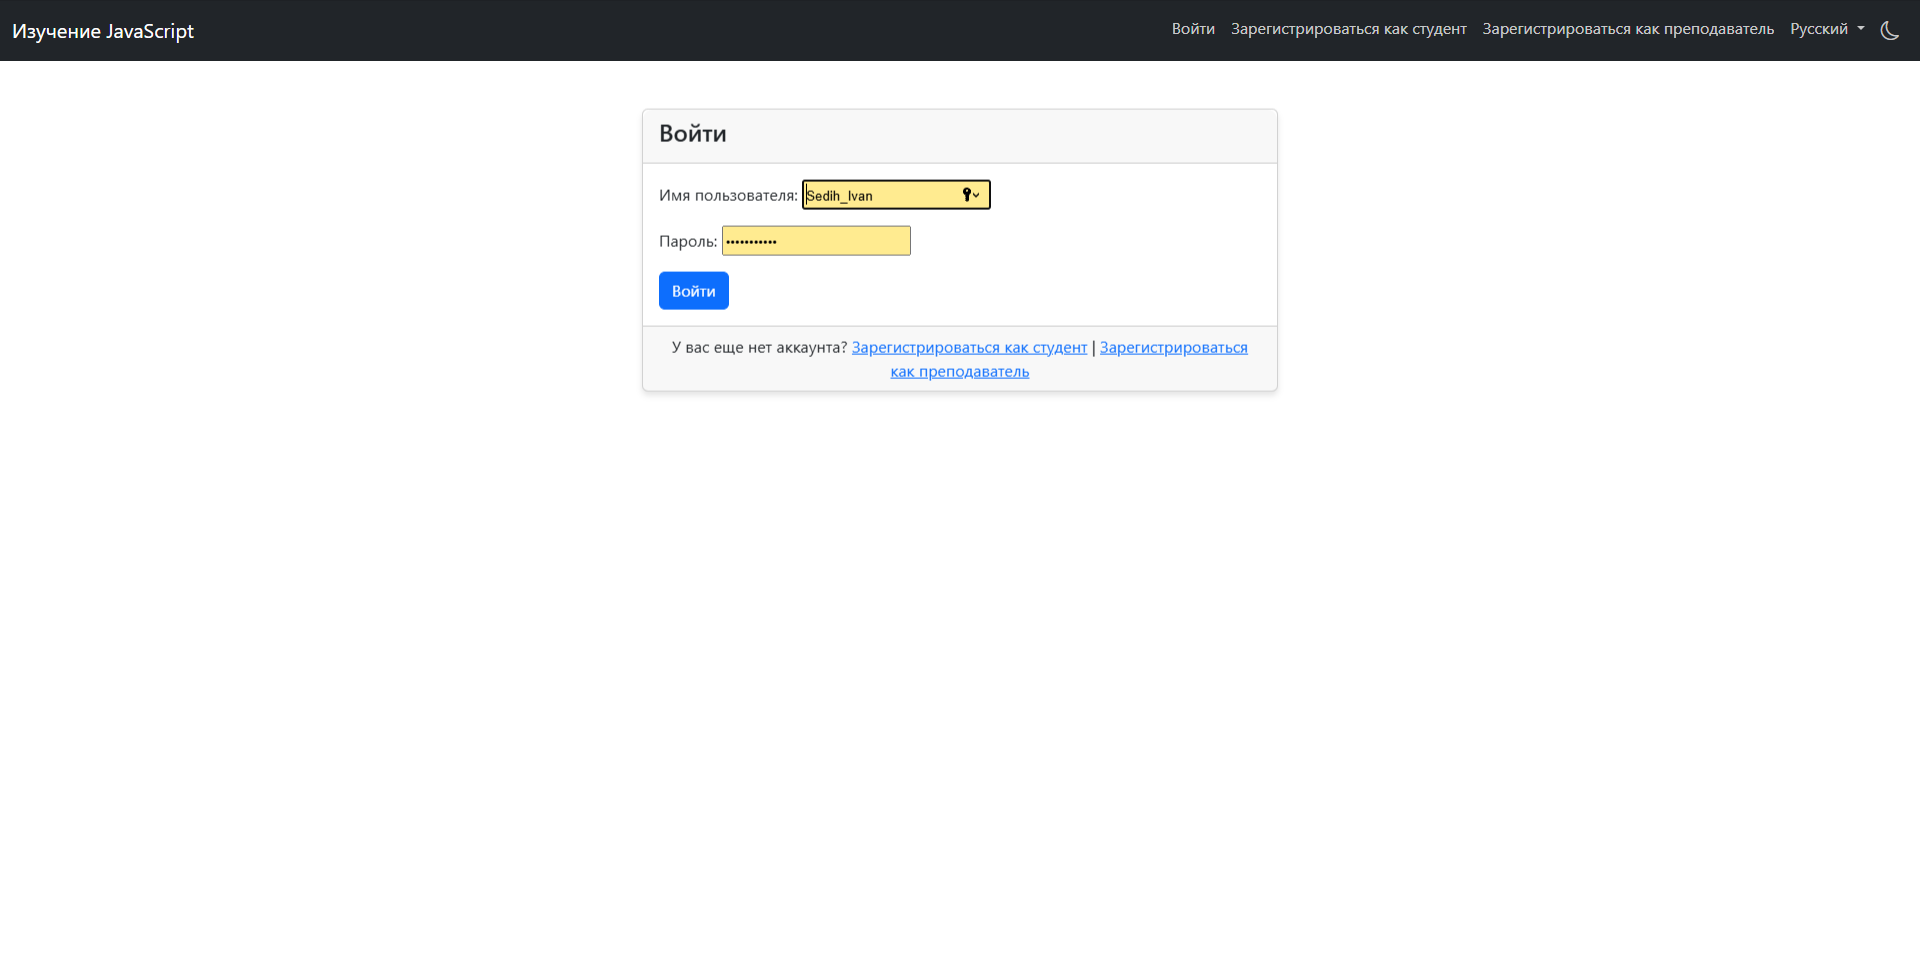
\includegraphics[width=0.9\textwidth]{images/регистр} 
		\caption{Регистрация и авторизация пользователя}
		\label{login:image}
	\end{figure}
	
\subsubsection{Создание курса и запись студента}
	
Описание: преподаватель должен иметь возможность создать новый курс, указав название, описание и изображение, а студент — записаться на существующий курс.
	
Ожидаемый результат: после создания курса он отображается в каталоге курсов, а студент, выбрав курс и нажав "Записаться", получает доступ к нему. При ошибке в данных (например, пустое название) система выдает предупреждение.
	
\begin{figure}[ht]
		\centering
		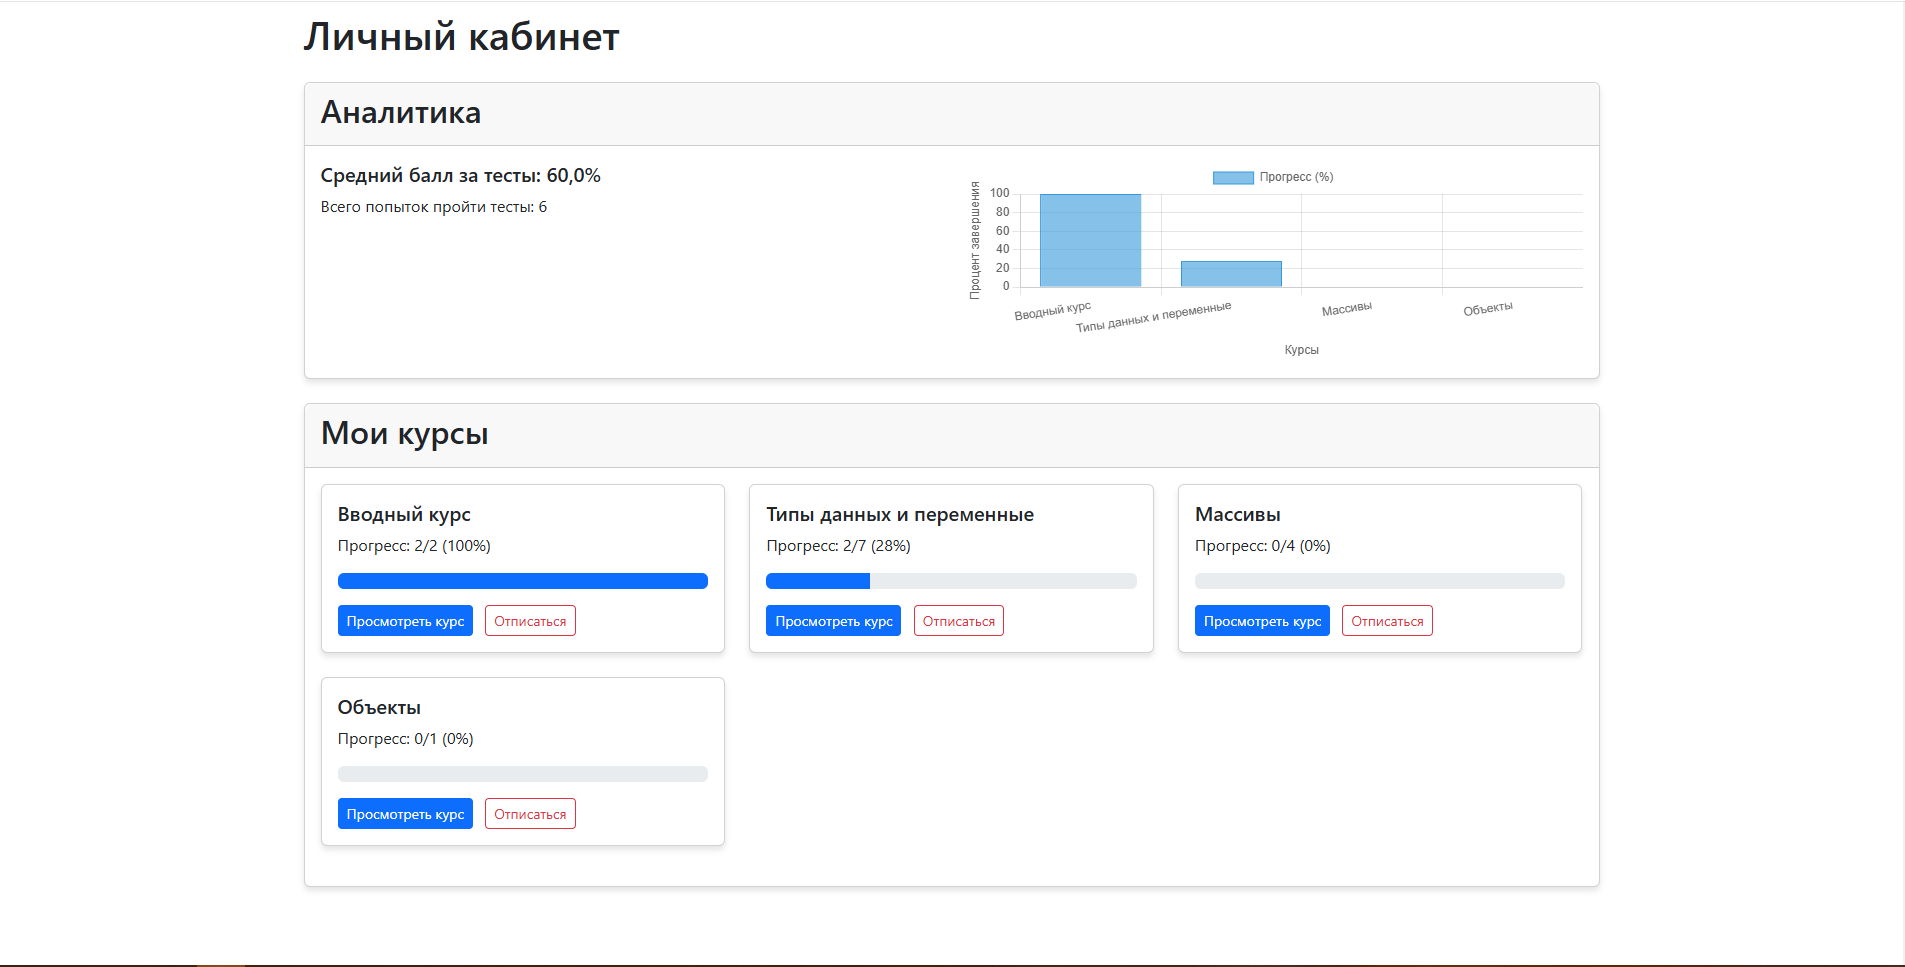
\includegraphics[width=0.9\textwidth]{images/запись} 
		\caption{Создание курса и запись студента}
		\label{enroll:image}
\end{figure}
	
\subsubsection{Добавление урока}
	
Описание: преподаватель должен иметь возможность добавить урок к курсу, используя CKEditor для редактирования контента (текст, видео, упражнения), с указанием порядка и статуса публикации.
	
Ожидаемый результат: урок успешно добавляется, контент отображается корректно для студентов после публикации. При отсутствии обязательных полей (например, названия) система выдает сообщение об ошибке.
	
	\begin{figure}[ht]
		\centering
		
\includegraphics[width=0.9\textwidth]{images/урокдобавить} 
		\caption{Добавление урока}
		\label{urok:image}
	\end{figure}
\newpage
\subsubsection{Прохождение теста и просмотр результатов}
	
Описание: студент должен иметь возможность пройти тест, связанный с уроком, выбрав ответы или введя текст, и просмотреть результат после завершения.
	
Ожидаемый результат: после сдачи теста отображаются баллы и статус (пройден/не пройден). При некорректных ответах система сохраняет результат и предлагает повторить попытку, если разрешено.
	
	\begin{figure}[ht]
		\centering
		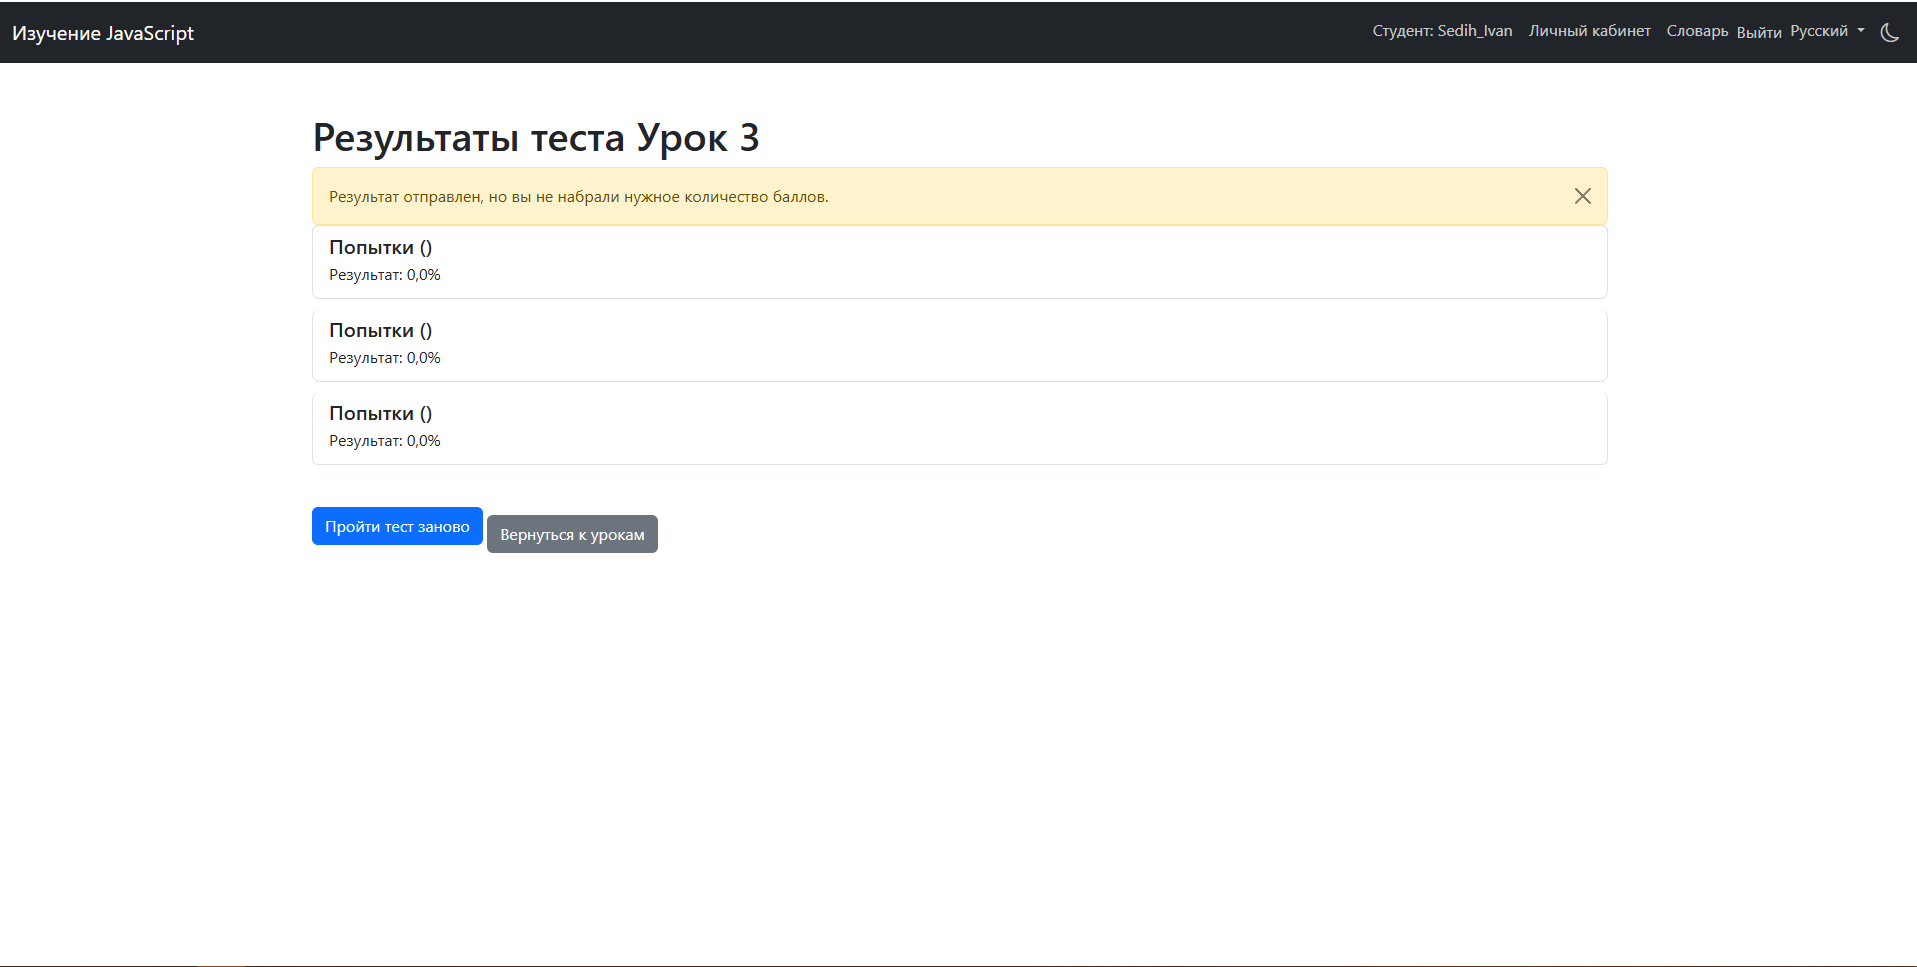
\includegraphics[width=0.9\textwidth]{images/тестрез} 
		\caption{Прохождение теста и результаты}
		\label{test:image}
	\end{figure}
	
\subsubsection{Присвоение достижения студенту}
	
Описание: система должна автоматически присваивать достижение студенту после выполнения определенного действия (например, завершения первого урока), а студент должен иметь возможность просмотреть полученные достижения в своем профиле.
	
Ожидаемый результат: после завершения урока система регистрирует достижение (например, "Первый завершённый урок") и отображается его в профиле студента. При ошибке (например, если достижение не настроено) система уведомляет администратора, но не прерывает работу.
	
	\begin{figure}[ht]
		\centering
		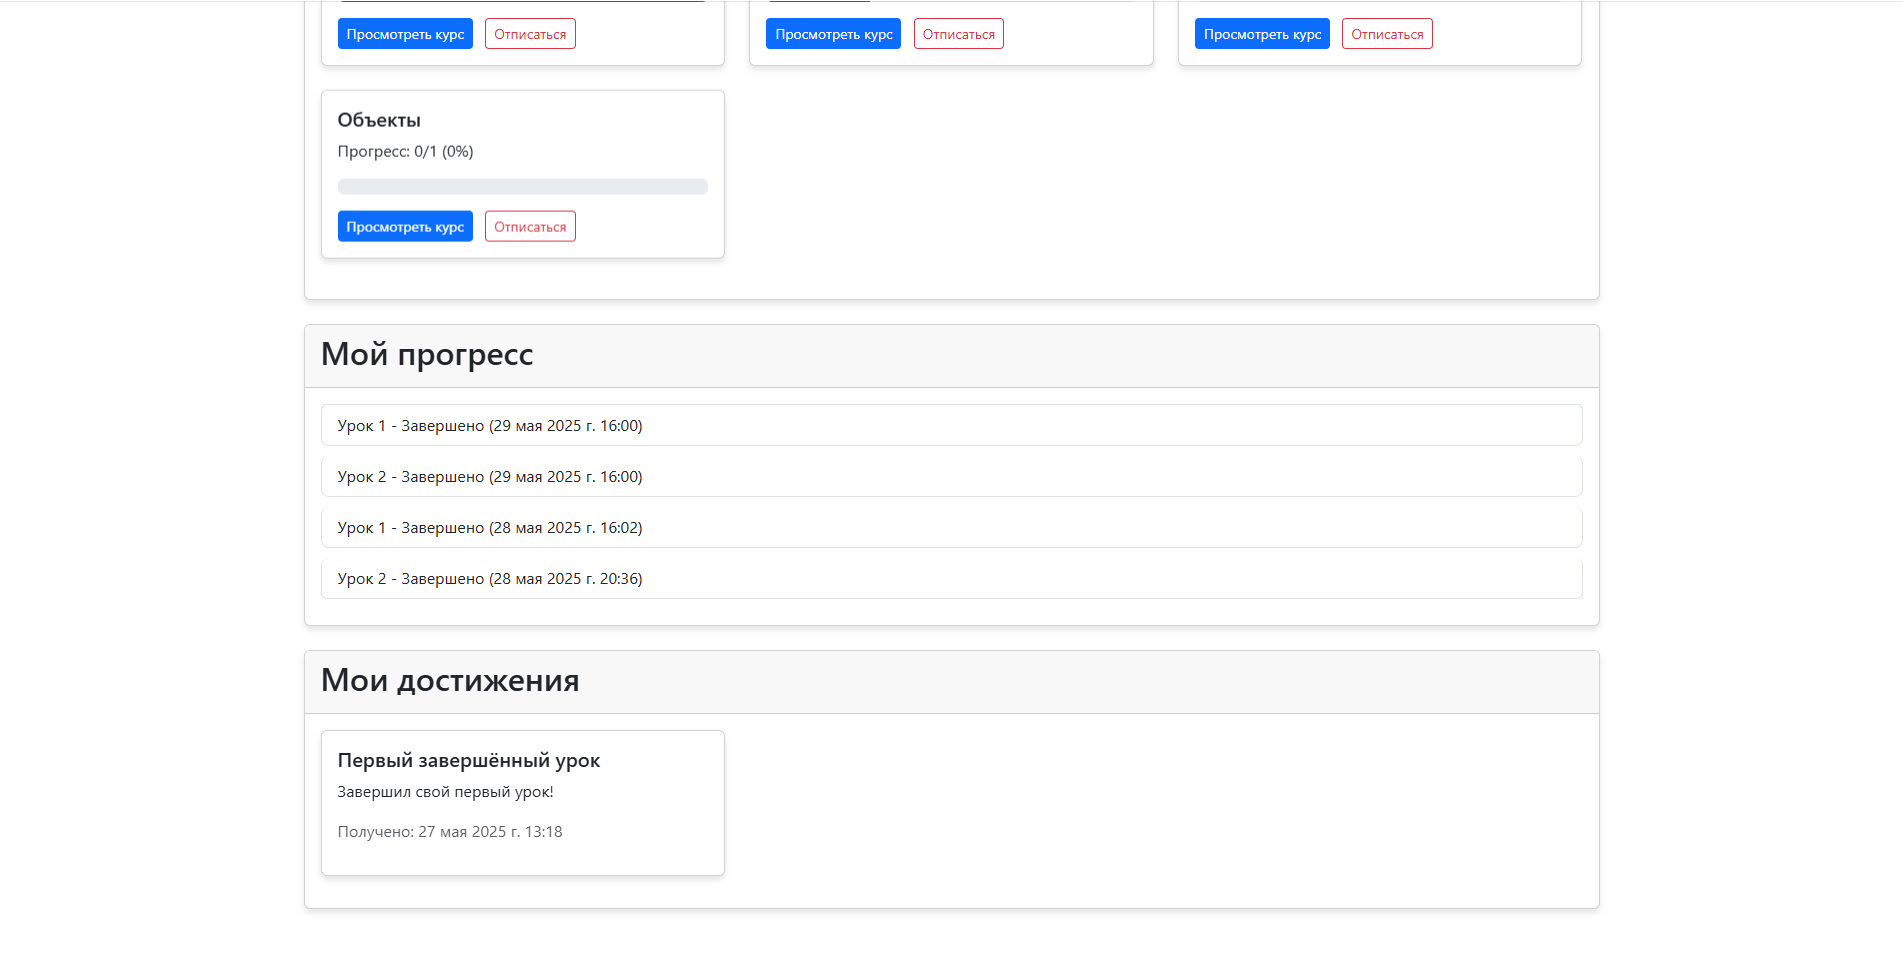
\includegraphics[width=0.9\textwidth]{images/достижение} 
		\caption{Присвоение достижения студенту}
		\label{achiv:image}
	\end{figure}
	
\subsubsection{Редактирование курса}
	
Описание: преподаватель должен иметь возможность редактировать существующий курс, изменяя его название, описание, изображение или статус публикации.
	
Ожидаемый результат: после редактирования изменения сохраняются, и обновленный курс отображается в каталоге курсов. При ошибке (например, пустое название) система выдает предупреждение.
	
	\begin{figure}[ht]
		\centering
		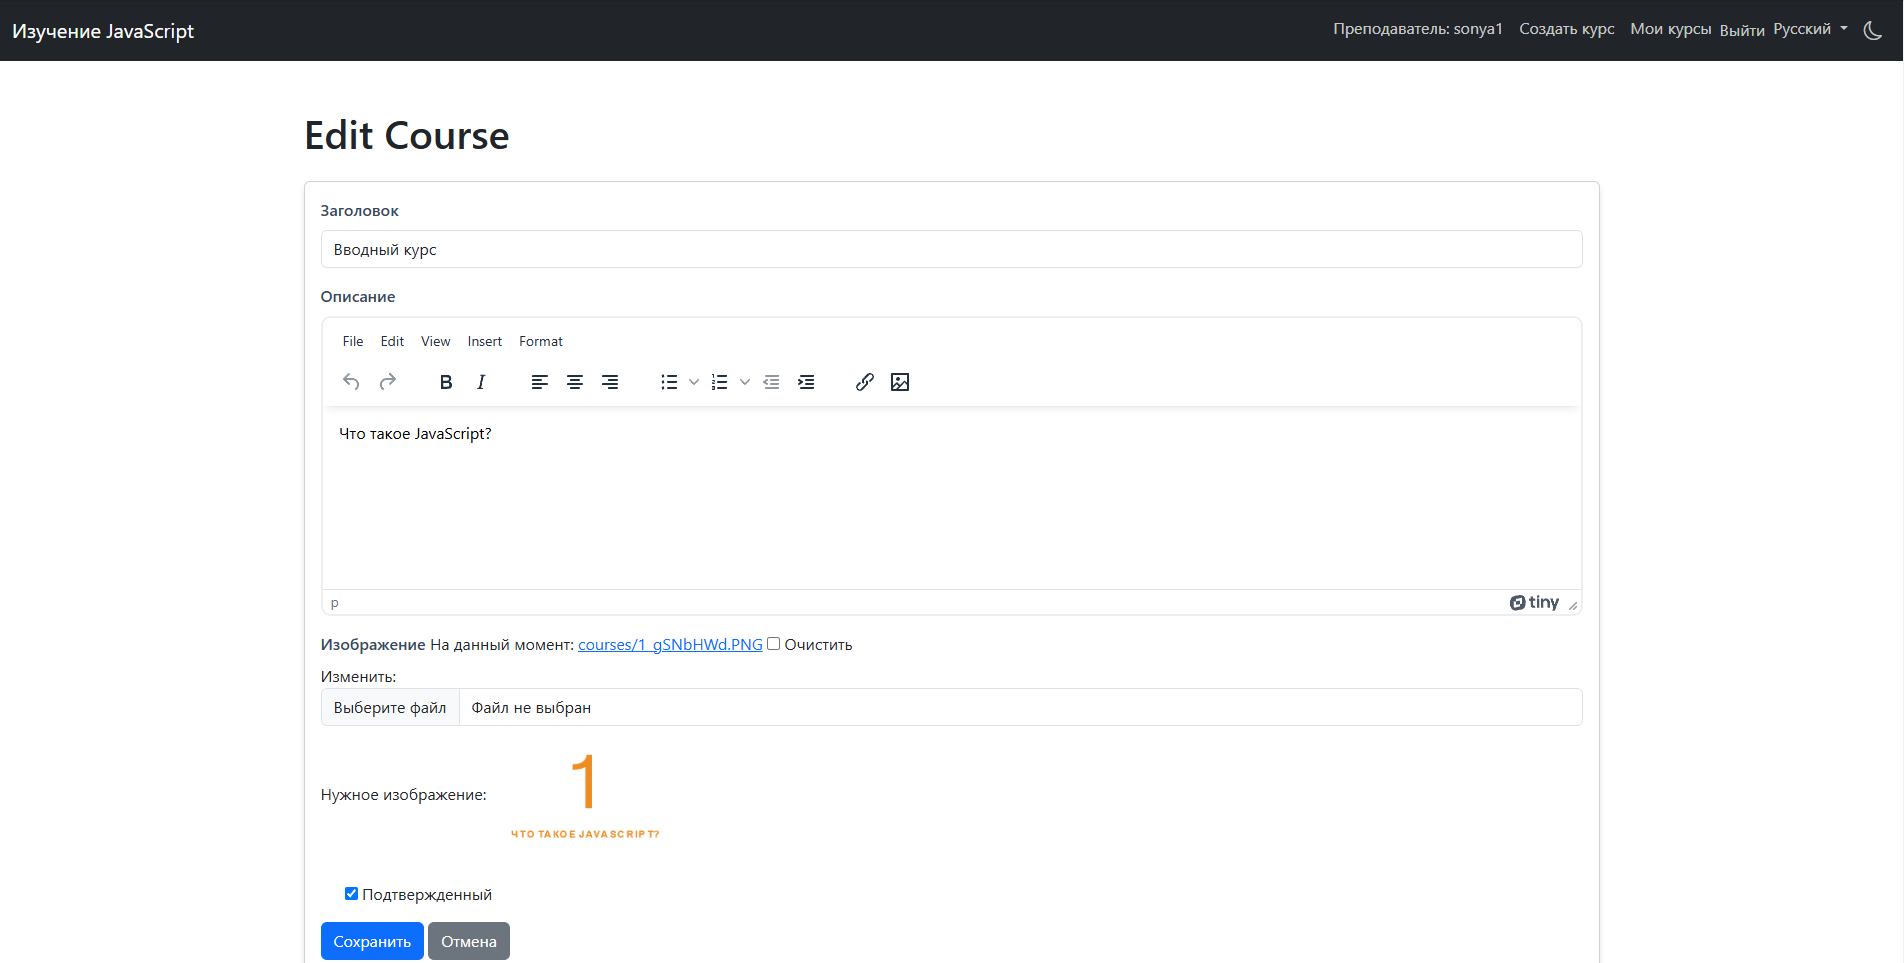
\includegraphics[width=0.9\textwidth]{images/редактироватькурс} 
		\caption{Редактирование курса}
		\label{editcourse:image}
	\end{figure}
	
\subsubsection{Удаление курса}
	
Описание: преподаватель должен иметь возможность удалить курс, при этом связанные данные (уроки, тесты) удаляются каскадно.
	
Ожидаемый результат: курс удаляется из системы, он больше не отображается в каталоге курсов, связанные уроки и тесты также удалены. При отсутствии прав (например, пользователь не является создателем курса) система выдает сообщение об ошибке.
	
	\begin{figure}[ht]
		\centering
		
\includegraphics[width=0.9\textwidth]{images/удалитькурс} 
		\caption{Удаление курса}
		\label{deletecourse:image}
	\end{figure}
	
\subsubsection{Проверка доступа к уроку}
	
Описание: система должна ограничивать доступ студента к уроку, если предыдущий урок не завершен или тест не сдан.
	
Ожидаемый результат: студент не может открыть урок, если не выполнены условия доступа, и получает уведомление (например, "Завершите предыдущий урок"). При выполнении условий урок становится доступным.
	
	\begin{figure}[ht]
		\centering
		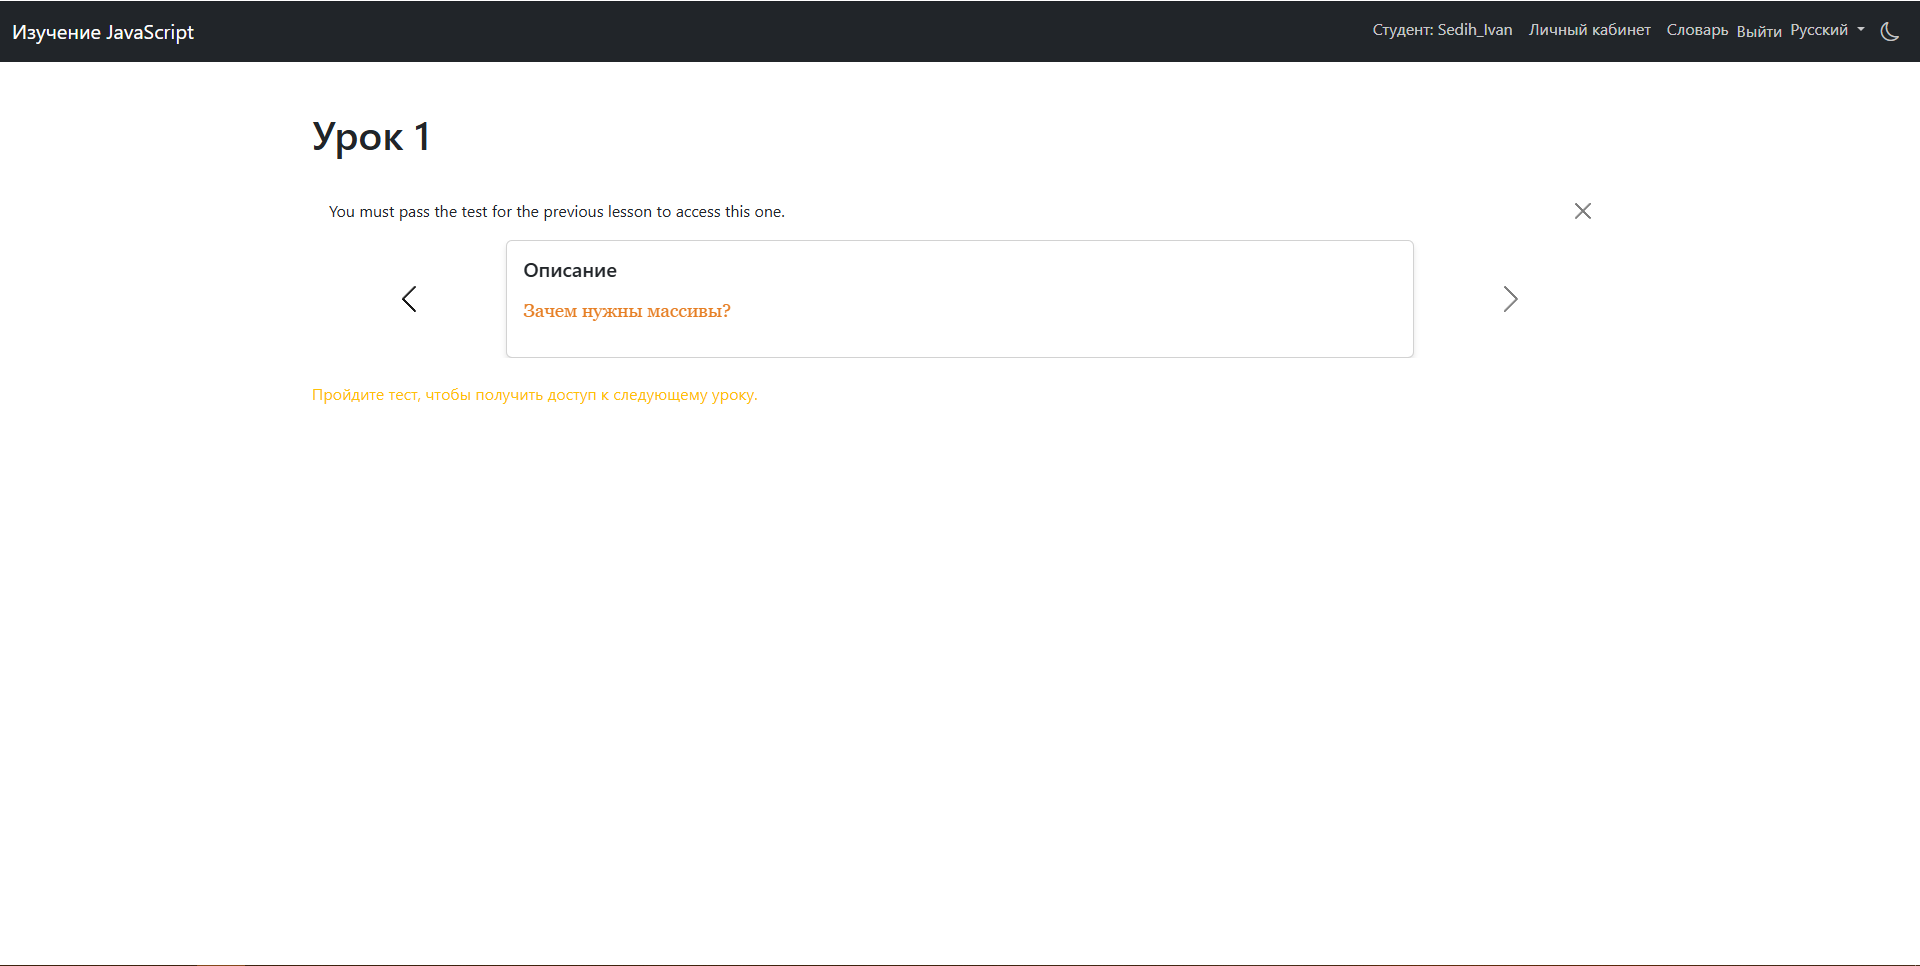
\includegraphics[width=0.9\textwidth]{images/доступурок} 
		\caption{Проверка доступа к уроку}
		\label{access:image}
	\end{figure}
	
\subsubsection{Просмотр прогресса студента}
	
Описание: студент должен иметь возможность просмотреть свой прогресс по курсу, включая завершенные уроки, результаты тестов и средний балл.
	
Ожидаемый результат: в панели студента отображаются завершенные уроки, результаты тестов и средний балл по курсу. При отсутствии данных (например, студент не начал курс) отображается соответствующее сообщение.
	
	\begin{figure}[ht]
		\centering
		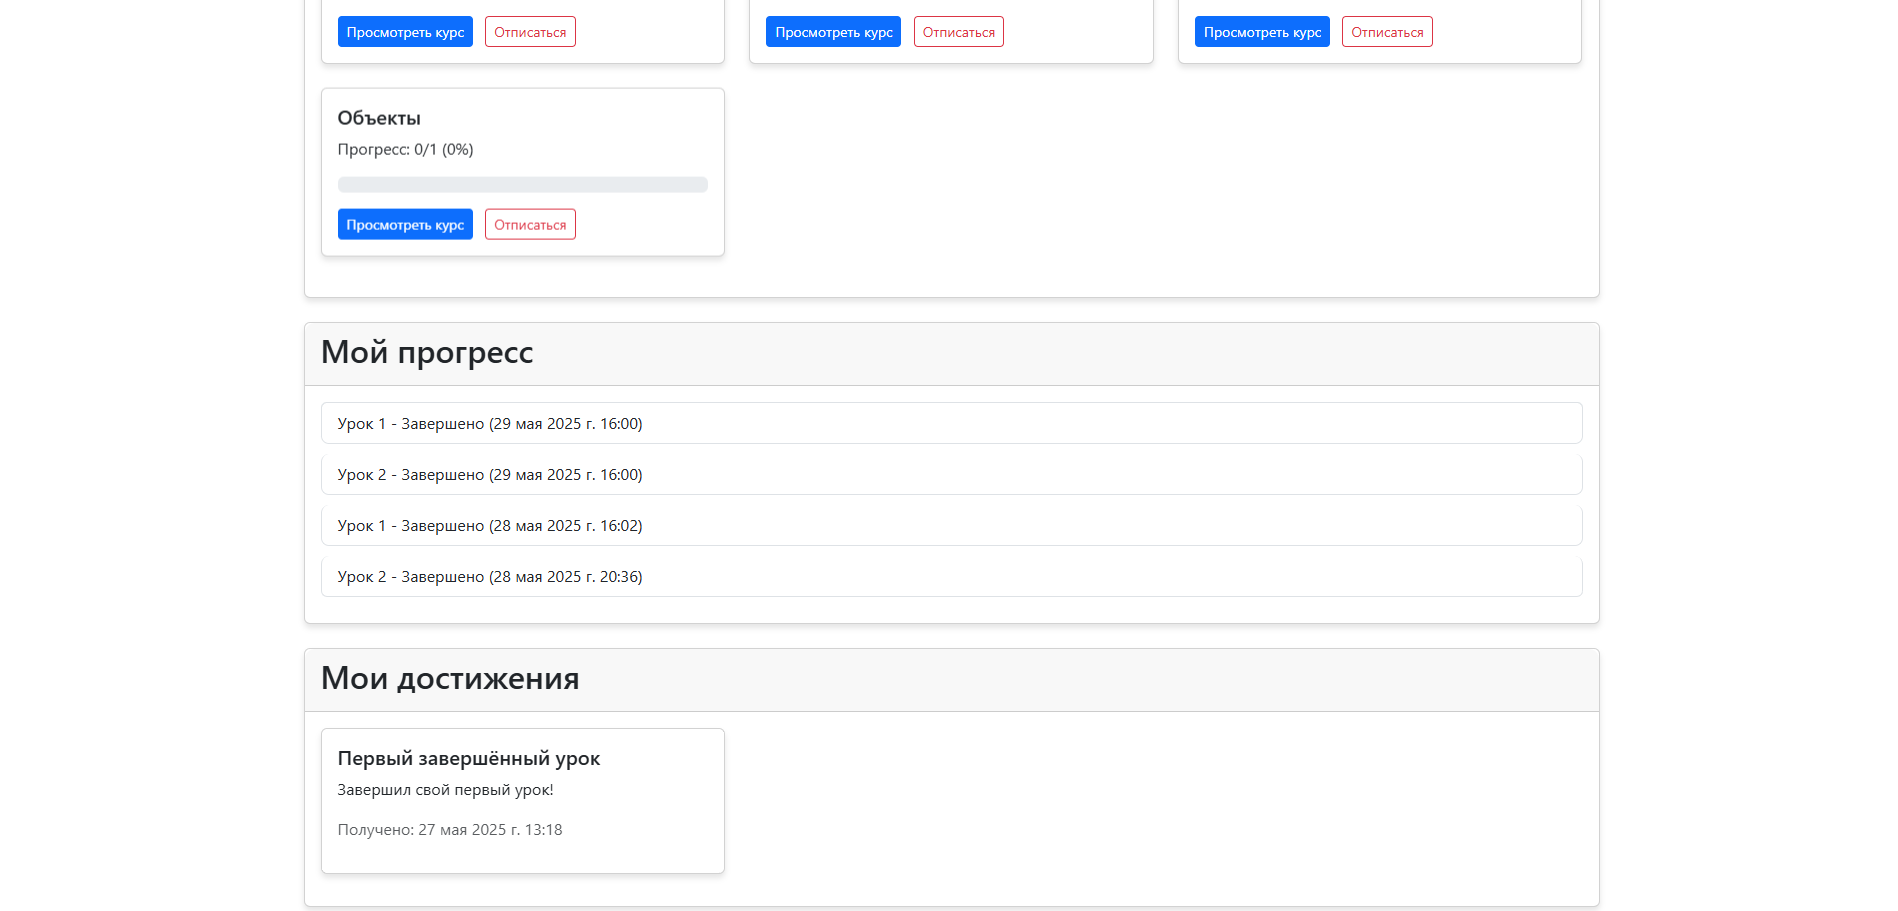
\includegraphics[width=0.9\textwidth]{images/прогресс} 
		\caption{Просмотр прогресса студента}
		\label{progress:image}
	\end{figure}
	

\subsubsection{Управление вопросами и ответами теста}
	
Описание: преподаватель должен иметь возможность добавить, редактировать и удалить вопросы и ответы теста, связанного с уроком.
	
Ожидаемый результат: вопросы и ответы успешно добавляются, редактируются или удаляются, изменения отражаются в тесте для студентов. При ошибке (например, некорректный тип вопроса) система выдает сообщение.
	
	\begin{figure}[ht]
		\centering
		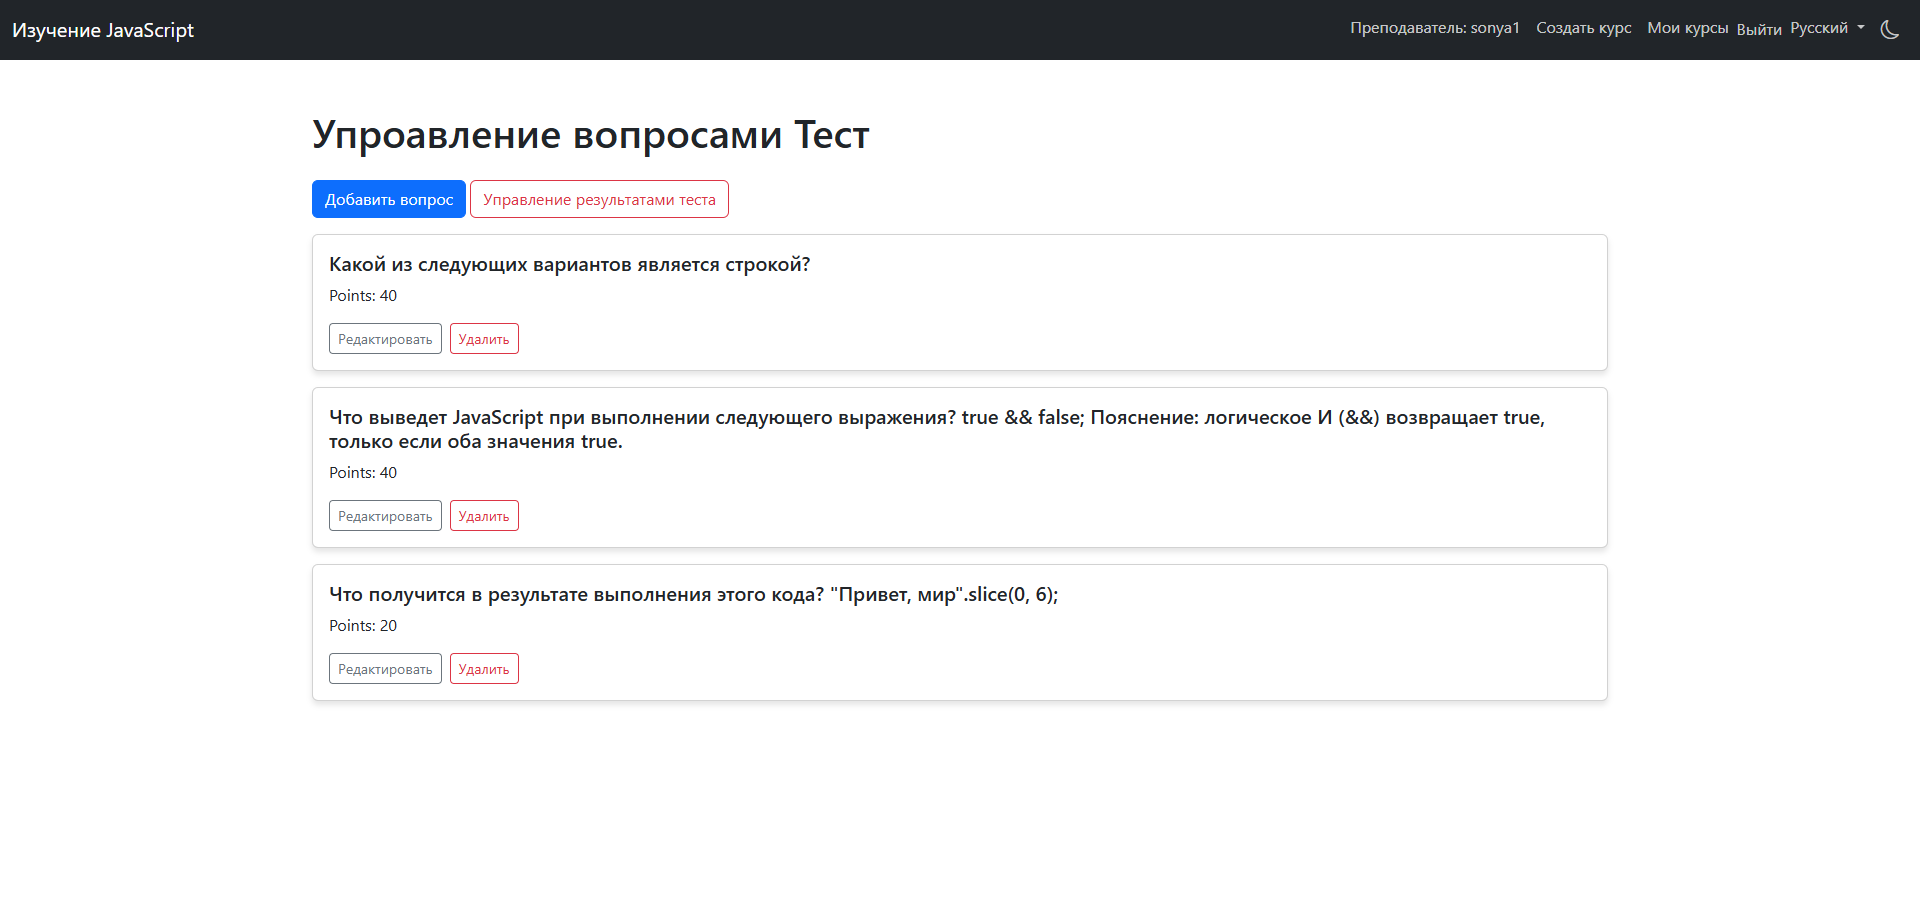
\includegraphics[width=0.9\textwidth]{images/вопросы} 
		\caption{Управление вопросами и ответами теста}
		\label{questions:image}
	\end{figure}

\begin{xltabular}{\textwidth}{|X|l|X|}
	\caption{Результаты системного тестирования\label{tab:system_testing_results}}\\
	\hline
	Сценарий & Статус & Описание \\ \hline
	\endfirsthead
	\continuecaption{Продолжение таблицы \ref{tab:system_testing_results}}\\
	\hline
	Сценарий & Статус & Описание \\ \hline
	\endhead
	Регистрация и авторизация & Успешно & Пользователи регистрируются и входят \\ \hline
	Создание и запись на курс & Успешно & Курс создаётся, студенты записываются \\ \hline
	Добавление урока & Успешно & Урок добавляется, контент отображается \\ \hline
	Прохождение теста & Успешно & Тесты проходятся, результаты сохраняются \\ \hline
	Присвоение достижения & Успешно & Достижение присваивается, отображается в профиле \\ \hline
	Редактирование курса & Успешно & Курс редактируется, изменения сохраняются \\ \hline
	Удаление курса & Успешно & Курс и связанные данные удаляются \\ \hline
	Переупорядочивание уроков & Успешно & Уроки переупорядочиваются корректно \\ \hline
	Проверка доступа к уроку & Успешно & Доступ ограничивается по условиям \\ \hline
	Просмотр прогресса студента & Успешно & Прогресс отображается в панели студента \\ \hline
	Управление вопросами и ответами & Успешно & Вопросы и ответы редактируются корректно \\ \hline
\end{xltabular}

Результаты: все сценарии выполнены успешно, система работает стабильно, критических ошибок не выявлено. Функциональность соответствует заявленным требованиям, обеспечивая удобство использования для преподавателей и студентов в рамках образовательных процессов. Тестирование подтвердило надежность платформы, включая обработку ошибок, ограничение доступа и управление контентом курсов.

\subsection{Сборка компонентов системы}

Для сборки и запуска веб-приложения нужно выполнить следующие шаги:

\begin{enumerate}
	\item Установка окружения:
	\begin{itemize}
		\item установите Python 3.9+ и pip.
		\item склонируйте репозиторий: git clone https://github.com/Seduk23/DiplomFinal.git;
		\item перейдите в директорию проекта: cd DiplomFinal;
		\item создайте и активируйте виртуальное окружение: python -m venv venv и venv\textbackslash Scripts\textbackslash activate (Windows) или source venv/bin/activate (Linux/macOS);
		\item установите зависимости: pip install -r requirements.txt.
	\end{itemize}
	
	\item Настройка базы данных:
	\begin{itemize}
		\item используется SQLite по умолчанию. Для PostgreSQL настройте settings.py и установите psycopg2-binary;
		\item выполните миграции: python manage.py makemigrations и python manage.py migrate.
	\end{itemize}
	
	\item Настройка окружения:
	\begin{itemize}
		\item создайте файл .env с настройками: SECRETKEY=yoursecretkey, DEBUG=True.
	\end{itemize}
	
	\item Подключение библиотек:
	\begin{itemize}
		\item CKEditor: установлен через pip install django-ckeditor;
		\item AOS и Bootstrap: подключены через CDN в base.html.
	\end{itemize}
	
	\item Настройка медиафайлов:
	\begin{itemize}
		\item в settings.py добавьте: MEDIAURL='/media/', MEDIAROOT=BASEDIR / 'media'.
	\end{itemize}
	
	\item Локализация:
	\begin{itemize}
		\item настройте LANGUAGES и LOCALEPATHS в settings.py;
		\item скомпилируйте переводы: python manage.py compilemessages.
	\end{itemize}
	
	\item Запуск:
	\begin{itemize}
		\item соберите статические файлы: python manage.py collectstatic;
		\item создайте суперпользователя: python manage.py createsuperuser;
		\item запустите сервер: python manage.py runserver.
	\end{itemize}
\end{enumerate}
   \section*{ЗАКЛЮЧЕНИЕ}
\addcontentsline{toc}{section}{ЗАКЛЮЧЕНИЕ}

Преимущества аддитивных технологий заключается в разнообразии процессов, позволяющих применять их в различных областях производства. Существенным ограничением же является и экономическая составляющая, которая не позволит внедрить аддитивное производство повсеместно.
  
Компании, видя, как развиваются информационные технологии, пытаются использовать их выгодно для своего бизнеса, запуская свой сайт для того, чтобы заявить о своем существовании, проинформировать потенциального клиента об услугах или продуктах, которые предоставляет. 
Для продвижения компании «Русатом – Аддитивные технологии» был разработан веб-сайт на основе системы «1С-Битрикс: Управление сайтом».

Основные результаты работы:

\begin{enumerate}
\item Проведен анализ предметной области. Выявлена необходимость использовать 1С-Битрикс.
\item Разработана концептуальная модель web-сайта. Разработана модель данных системы. Определены требования к системе.
\item Осуществлено проектирование web-сайта. Разработана архитектура серверной части. Разработан пользовательский интерфейс web-сайта.
\item Реализован и протестирован web-сайт. Проведено модульное и системное тестирование.
\end{enumerate}

Все требования, объявленные в техническом задании, были полностью реализованы, все задачи, поставленные в начале разработки проекта, были также решены.

Готовый рабочий проект представлен адаптивной версткой сайта. Сайт находится в публичном доступе, поскольку опубликован в сети Интернет.  

}\fi
\addcontentsline{toc}{section}{СПИСОК ИСПОЛЬЗОВАННЫХ ИСТОЧНИКОВ}

\begin{thebibliography}{9}

    \bibitem{javascript5} Бейли, Р. Методика преподавания программирования иностранным студентам / Р. Бейли. – Москва: Лань, 2021. – 210 с. – ISBN 978-5-8114-5678-9. – Текст~: непосредственный.
    
    \bibitem{javascript1} Браун, И. Изучаем JavaScript: руководство по созданию современных веб-сайтов / И. Браун. – Москва: Эксмо, 2022. – 480 с. – ISBN 978-5-04-123456-7. – Текст~: непосредственный.
    
    \bibitem{css1} Веру, Л. CSS-секреты. 47 советов по улучшению веб-интерфейсов / Л. Веру. – Санкт-Петербург: Питер, 2017. – 368 с. – ISBN 978-5-496-02699-4. – Текст~: непосредственный.
    
    \bibitem{html1}	Голдстайн, А. HTML5 и CSS3 для всех / А. Голдстайн, Л. Лазарис, Э. Уэйл. – Москва~: Вильямс, 2012. – 368 с. – ISBN 978-5-699-57580-0. – Текст~: непосредственный.
    
    \bibitem{htmlcss} Дэкетт, Д. HTML и CSS. Разработка и создание веб-сайтов / Д. Дэкетт. – Москва: Эксмо, 2014. – 480 с. – ISBN 978-5-699-64193-2. – Текст~: непосредственный.
	
    \bibitem{javascript2} Кантор, Д. JavaScript для начинающих: от основ до веб-приложений / Д. Кантор. – Санкт-Петербург: Питер, 2023. – 360 с. – ISBN 978-5-4461-2345-2. – Текст~: непосредственный.
    
    \bibitem{sqlite} Кинг, Д. SQLite. Руководство разработчика / Д. Кинг. – Москва: Вильямс, 2021. – 256 с. – ISBN 978-5-8459-1876-3. – Текст~: непосредственный.
    
    \bibitem{js3} Кларк, А. Технологии адаптивного обучения в IT-образовании / А. Кларк. – Санкт-Петербург: БХВ, 2022. – 180 с. – ISBN 978-5-9775-0987-6. – Текст~: непосредственный.
    
    \bibitem{javascript3} Макфарланд, Д. JavaScript и jQuery: интерактивная фронтенд-разработка / Д. Макфарланд. – Москва: Диалектика, 2021. – 512 с. – ISBN 978-5-907203-45-6. – Текст: непосредственный.  

    \bibitem{python1} Матей, Н. Python. К вершинам мастерства / Н. Матей. – Санкт-Петербург: Питер, 2022. – 432 с. – ISBN 978-5-4461-0926-5. – Текст~: непосредственный.
	
	\bibitem{python} Петров, И. П. Python для веб-разработки: от основ до продвинутых техник / И. П. Петров. – Санкт-Петербург: Питер, 2024. – 416 с. – ISBN 978-5-4461-1789-5. – Текст~: непосредственный.
	
    \bibitem{javascript4} Симпсон, К. Глубокая работа с JavaScript: замыкания, прототипы, асинхронность / К. Симпсон. – Санкт-Петербург: Питер, 2022. – 288 с. – ISBN 978-5-4461-1987-5. – Текст~: непосредственный.  
	
	\bibitem{html2}	Титтел, Э. HTML5 и CSS3 для чайников / Э. Титтел, К. Минник. – Москва~: Вильямс, 2016 – 400 с. – ISBN 978-1-118-65720-1. – Текст~: непосредственный.
	
	\bibitem{django}	Холл, Б. Django. Разработка веб-приложений / Б. Холл.– Москва: ДМК Пресс, 2023.– 512 с. – ISBN 978-5-97060-789-0.– Текст~: непосредственный.
	
    \bibitem{css2} Юэнс, В. CSS. Карманный справочник / В. Юэнс. – Москва: Символ-Плюс, 2020. – 272 с. – ISBN 978-5-93286-362-0. – Текст~: непосредственный.


\end{thebibliography}

\ifВКР{%\appendix{Представление графического материала}

Графический материал, выполненный на отдельных листах,
изображен на рисунках А.1--А.\arabic{числоПлакатов}.
\setcounter{числоПлакатов}{0}

\renewcommand{\thefigure}{А.\arabic{figure}} % шаблон номера для плакатов

\begin{landscape}
\begin{плакат}
	\centering
    \includegraphics[width=0.8\linewidth]{Ramka1}
    \заголовок{Сведения о ВКРБ}
    \label{pl1:image}      
\end{плакат}

\begin{плакат}
	\centering
    \includegraphics[width=0.8\linewidth]{Цели}
    \заголовок{Цель и задачи разработки}
    \label{pl2:image}      
\end{плакат}

\begin{плакат}
	\centering
    \includegraphics[width=0.8\linewidth]{Ramkaconcept}
    \заголовок{Концептуальная модель сайта}
    \label{pl3:image}      
\end{плакат}

\begin{плакат}
	\centering
    \includegraphics[width=0.8\linewidth]{RamkaUML}
    \заголовок{Диаграмма прецедентов}
    \label{pl4:image}      
\end{плакат}

\begin{плакат}
	\centering
	\includegraphics[width=0.8\linewidth]{компоненты}
	\заголовок{Диаграмма компонентов}
	\label{pl5:image}      
\end{плакат}

\begin{плакат}
	\centering
	\includegraphics[width=0.8\linewidth]{РегАвт}
	\заголовок{Страница регистрации и авторизации}
	\label{pl6:image}      
\end{плакат}

\begin{плакат}
	\centering
	\includegraphics[width=0.8\linewidth]{Главная}
	\заголовок{Главная страница}
	\label{pl7:image}      
\end{плакат}

\begin{плакат}
	\centering
	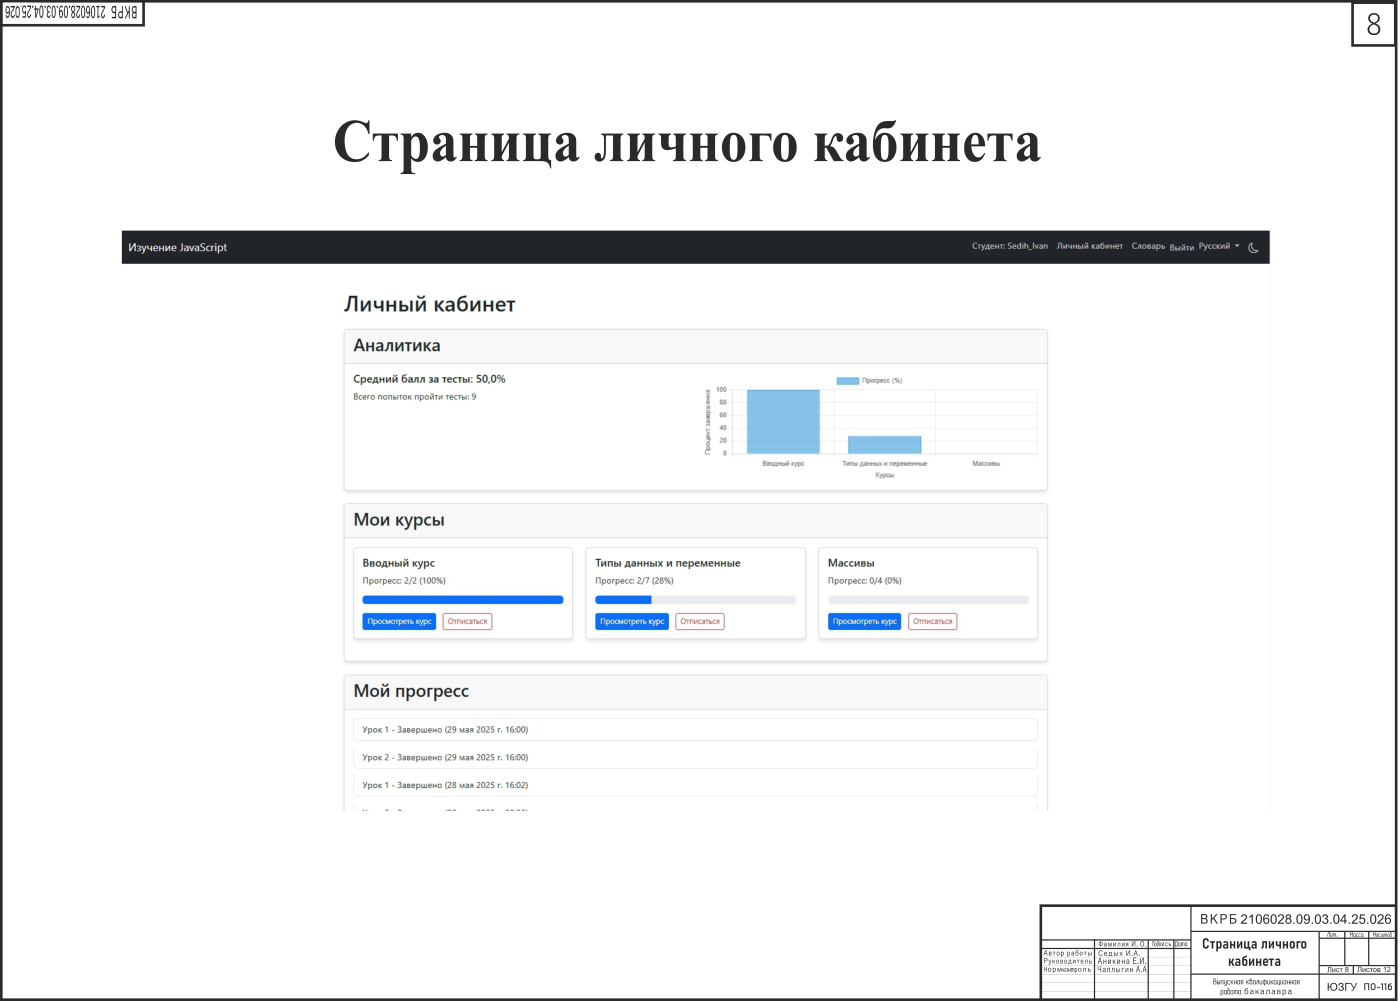
\includegraphics[width=0.8\linewidth]{кабинет}
	\заголовок{Личный кабинет}
	\label{pl8:image}      
\end{плакат}

\begin{плакат}
	\centering
	\includegraphics[width=0.8\linewidth]{добурок}
	\заголовок{Страница добавления урока}
	\label{pl9:image}      
\end{плакат}

\begin{плакат}
	\centering
	\includegraphics[width=0.8\linewidth]{урокзадание}
	\заголовок{Страница урока и задания}
	\label{pl10:image}
\end{плакат}

\begin{плакат}
	\centering
	\includegraphics[width=0.8\linewidth]{резытестов}
	\заголовок{Страница результатов тестов}
	\label{pl11:image}      
\end{плакат}

\begin{плакат}
	\centering
	\includegraphics[width=0.8\linewidth]{заключение}
	\заголовок{Заключение}
	\label{pl12:image}      
\end{плакат}
\end{landscape}
}\fi
\ifПрактика{}\else{\appendix{Фрагменты исходного кода программы}

main.tex
\lstinputlisting[language=Tex, frame=none]{main.tex}

ТехПроект.tex
\lstinputlisting[language=Tex, frame=none]{ТехПроект.tex}

\ifВКР{
\newpage
\addcontentsline{toc}{section}{На отдельных листах (CD-RW в прикрепленном конверте)}
\noindent
\begin{tabular}{p{5.8cm}C{4.8cm}C{4.8cm}}
   Автор ВКР & \lhrulefill{\fill} & \fillcenter\Автор \\
            \setarstrut{\footnotesize}
           & \footnotesize{(подпись, дата)} & \\
            \restorearstrut
   Руководитель ВКР & \lhrulefill{\fill} & \fillcenter\Руководитель \\
            \setarstrut{\footnotesize}
           & \footnotesize{(подпись, дата)} & \\
            \restorearstrut
   Нормоконтроль & \lhrulefill{\fill} & \fillcenter\Нормоконтроль \\
            \setarstrut{\footnotesize}
           & \footnotesize{(подпись, дата)} & \\
            \restorearstrut
\end{tabular}
\vskip 2cm
\begin{center}
\textbf{Место для диска}
\end{center}
}\fi
}\fi
\end{document}
